\pdfoutput=1
\documentclass[11pt]{amsart}
\usepackage{amsmath,amssymb,amsthm}
\usepackage[margin=1.2in]{geometry}
\usepackage{booktabs,adjustbox,graphicx,xcolor}
\usepackage[colorlinks=true,linkcolor=blue,citecolor=blue,urlcolor=blue]{hyperref}
\hypersetup{pdfauthor={Bernd Johannes Wuebben},
 pdftitle={Hermitian--Yang--Mills dynamics and harmonic moduli near a conifold}}
\setlength{\emergencystretch}{2em}
\newtheorem{theorem}{Theorem}[section]
\newtheorem{proposition}[theorem]{Proposition}
\newtheorem{lemma}[theorem]{Lemma}
\newtheorem{corollary}[theorem]{Corollary}
\theoremstyle{definition}
\newtheorem{definition}[theorem]{Definition}
\newtheorem{example}[theorem]{Example}
\theoremstyle{remark}
\newtheorem{remark}[theorem]{Remark}
\newcommand{\RR}{\mathbb R}
\newcommand{\CC}{\mathbb C}
\newcommand{\ZZ}{\mathbb Z}
\newcommand{\QQ}{\mathbb Q}
\newcommand{\PP}{\mathbb P}
\newcommand{\OO}{\mathcal O}
\newcommand{\cA}{\mathcal A}
\newcommand{\cH}{\mathcal H}
\newcommand{\cL}{\mathcal L}
\newcommand{\dd}{\mathrm d}
\DeclareMathOperator{\im}{im}
\DeclareMathOperator{\rank}{rank}
\DeclareMathOperator{\tr}{tr}
\DeclareMathOperator{\pr}{pr}
\DeclareMathOperator{\Vol}{Vol}
\DeclareMathOperator{\Eig}{Eig}
\DeclareMathOperator{\Dom}{Dom}
\title[HYM dynamics and harmonic moduli near a conifold]
{Hermitian--Yang--Mills dynamics and harmonic moduli near a conifold}
\author{Bernd Johannes Wuebben}
\subjclass[2020]{53C07 (primary); 14J32, 32Q25, 58J35 (secondary)}
\keywords{Hermitian--Yang--Mills flow, conifold degeneration,
Hermitian--Einstein metric, relative spectrum, harmonic moduli metric}
\date{November 12, 2026\\This version: November 12, 2026}

\DeclareMathOperator{\End}{End}
\DeclareMathOperator{\Hom}{Hom}
\DeclareMathOperator{\Ext}{Ext}
\DeclareMathOperator{\Herm}{Herm}
\DeclareMathOperator{\GL}{GL}
\DeclareMathOperator{\Aut}{Aut}
\DeclareMathOperator{\diag}{diag}
\newcommand{\dbar}{\bar\partial}
\newcommand{\cE}{\mathcal E}
\newcommand{\cV}{\mathcal V}
\newcommand{\cX}{\mathcal X}
\newcommand{\cP}{\mathcal P}
\newcommand{\cK}{\mathcal K}

\begin{document}
\begin{abstract}
We construct a nonflat rank-four bundle family on compact Calabi--Yau
threefolds smoothing eight ordinary double points and compare its
Hermitian--Einstein metrics, metric flow and local moduli geometry
uniformly through degeneration. A two-arrow matrix form determines all
seven small trace-free endomorphism eigenvalues with relative error,
including changing kernels and arbitrarily separated positive rates.
On each polystable member, an open spatial $C^1$ basin admits a finite
invariant graph and an initial phase for which the actual
Hermitian--Yang--Mills flow tracks an exact graph trajectory with
exponentially decaying $C^1$ error for all time. At the Hermitian--Einstein
equilibrium, the Hessian of twice Donaldson's functional restricted to
the graph is relatively equivalent to the same matrix form in the
original metric coordinates. We also identify the actual local bundle classes and
compare their harmonic metric on every stabilizer stratum. For paths
confined to this locus, the unique metric tangent cone at the split
bundle is $(\mathbb C^2,4|\mathrm du|^2)/((\mathbb Z/2)^2\rtimes S_2)$.
All comparisons allow independent node and bundle scales.
\end{abstract}
\maketitle
\section{Introduction}
\label{sec:introduction}

Near a polystable bundle, a finite-dimensional deformation
space describes the loss of rigidity of Hermitian--Einstein
metrics. When the underlying Kähler manifold also degenerates,
this description requires estimates uniform in the geometric
parameters. An additive error in a finite operator is
insufficient if some eigenvalues are much smaller than
others. Likewise, a stationary reduction alone does not
determine the trajectory selected by a spatially varying
initial metric or the harmonic metric on nearby bundle
classes. This paper proves these three comparisons on one
nonflat bundle family over compact conifold smoothings.

\subsection{The geometric family and the principal theorem}

We use a polarized family $X_p$ of Calabi--Yau threefolds
whose central fibre has eight ordinary double points.
The base is a small ball in the six-dimensional space
\begin{equation}\label{eq:intro-base}
 \mathcal R=\left\{p\in\CC^8:
       \sum_{i\in I_f}p_i=\sum_{i\in I_g}p_i=0\right\},
 \qquad |I_f|=|I_g|=4.
\end{equation}
Its smooth locus is the complement of the eight coordinate
hyperplanes. The node parameters satisfy
$\tau_i(p)=p_i/u_i(p)$ for nonvanishing holomorphic units.
The smooth fibres are complete intersections of bidegrees
$(1,1),(1,1),(2,2)$ in $\PP^3\times\PP^3$.
Write $H=\OO(2,2)$ and $L=\OO(1,-1)$ on each fibre.
The actual Ricci-flat metric in $c_1(H)$ has volume
$V=160/3$, and the split bundle is
\[
                 E^{\rm sp}=L\otimes\CC^2\oplus L^{-1}\otimes\CC^2.
\]
The polarized construction and the uniform actual-metric
input are restated in Section~\ref{sec:geometry} from
\cite{W_Hodge}. All subsequent bundle and flow estimates
are proved here.

The bundle deformation parameters are two matrices
$z=(A,B)\in W=\operatorname{Mat}_2(\CC)\oplus\operatorname{Mat}_2(\CC)$,
with compact action
$(k_+,k_-)\cdot(A,B)=(k_+Ak_-^{-1},k_-Bk_+^{-1})$.
The two harmonic extension forms have squared norms
$c_+(p),c_-(p)>0$. They are uniformly bounded above
and below and converge to positive central values.
On the real seven-dimensional space
\[
 \mathfrak h=\{(S_+,S_-):S_\pm=S_\pm^*,\quad\tr S_++\tr S_-=0\}
\]
define the mass and energy
\begin{equation}\label{eq:intro-finite-pair}
 \begin{split}
 M(S)&=V(\tr S_+^2+\tr S_-^2),\\
 E_{p,z}(S)&=2c_+\|S_+A-AS_-\|_{\rm HS}^2
                  +2c_-\|S_-B-BS_+\|_{\rm HS}^2.
 \end{split}
\end{equation}
Let $\mu_1\le\cdots\le\mu_7$ be its generalized
eigenvalues, including zeros. The quadratic moment is
\[
 \mu_{2,p}(A,B)=V^{-1}
       (c_+AA^*-c_-B^*B,\ c_-BB^*-c_+A^*A).
\]
Its zero set becomes $XX^*=Y^*Y$, $YY^*=X^*X$
under $X=\sqrt{c_+}A$, $Y=\sqrt{c_-}B$.

\begin{theorem}\label{thm:main}
On the family above there is an actual holomorphic
rank-four bundle family $\mathcal E_{p,w}$ realizing
the full local deformation germ of $E^{\rm sp}$, with
$\det\mathcal E_{p,w}=\OO$ and $c_2(\mathcal E_{p,w})H=32$.
After one common shrink, the following hold uniformly
over every smooth $p$ and all small bundle parameters.

\smallskip\noindent
\textup{(i)} There is a real $K$-equivariant map
$\chi_p(z)=z+O(|z|^2)$, $d\chi_p=I+O(|z|)$, such that
every $z\in\mu_{2,p}^{-1}(0)$ gives an actual HE
connection on $\mathcal E_{p,\chi_p(z)}$.
These representatives cover the sufficiently small
polystable objects in the stated local germ. The germ
contains no stable rank-four objects.

\smallskip\noindent
\textup{(ii)} At these HE connections the positive
operator linearizing $h^{-1}\dot h=-2\mathrm i\Lambda F_h$
has complete small spectrum
\[
 (1-C|z|)\mu_j\le\lambda_j\le(1+C|z|)\mu_j
       \quad(1\le j\le7),\qquad\lambda_8\ge c>0.
\]
Its exact trace-free kernel is the compact infinitesimal
stabilizer. The comparison allows changing kernel dimension
and arbitrary ratios of positive eigenvalues.

\smallskip\noindent
\textup{(iii)} Fix an HE member, write $r=|\chi_p(z)|$,
and fix any finite graph regularity order $m\ge4$.
There is a common spatial $C^1$ basin of smooth
determinant-normalized initial metrics and a chosen
$C^m$ seven-dimensional invariant graph. Every flow
in that basin selects a $C^1$ finite initial phase
and tracks the corresponding exact graph trajectory
with error $CD_*e^{-ct}$ in the logarithmic $C^1$ norm.
Here $D_*$ is its initial displacement from the graph.
The selected graph trajectory remains in the actual
equation for all positive time. Its finite metric is
the pulled-back $L^2$ metric, its energy is twice
Donaldson's functional, and its Hessian at the HE
origin is relatively $1+O(|z|)$ equivalent to $E_{p,z}$
in the same $S$ coordinates. The preparation time
$4\sigma^{-1}\log(1/r)$ is negligible compared with
every positive inverse weak rate.

\smallskip\noindent
\textup{(iv)} The local HE classes are parametrized by
$\CC^2/\mathsf W$, where $\mathsf W=(\ZZ/2)^2\rtimes S_2$
acts by signs and permutation. On every quotient stratum,
their actual harmonic connection metric is relatively
$1+O(|u|)$ equivalent to $4|\dd u|^2$.
For paths confined to a fixed sufficiently small local
locus, its metric completion is the corresponding
closed parameter locus, and its unique tangent cone at
the split bundle is $(\CC^2,4|\dd u|^2)/\mathsf W$.
The rescaled distance error is $O(\rho)$ on bounded
balls, uniformly in the degenerating base.
\end{theorem}

The theorem combines the precise statements proved below.
The bundle realization is Proposition~\ref{prop:effective-bundles}.
The relative spectrum and exact balancing are
Theorem~\ref{thm:complete-bundle-spectrum} and
Proposition~\ref{prop:exact-balancing-coordinates};
Section~\ref{sec:balancing} proves holomorphic
polystability and local completeness. The dynamical
claims are Theorems~\ref{thm:spatial-entry},
\ref{thm:invariant-graph}, \ref{thm:all-time-tracking}
and Corollary~\ref{cor:relative-finite-hessian}.
The actual quotient identification, harmonic metric and
distance are Theorems~\ref{thm:unitary-rigidity},
\ref{thm:harmonic-quotient} and \ref{thm:metric-cone}.
Their proofs use the same connections and the same
compact action. The flow parameters are fixed along
each trajectory; uniformity permits them to approach
their limits jointly when comparing different trajectories.

The balanced normal form has two cycle parameters.
Its four types have trace-free stabilizer dimensions
$1,3,2,7$: two distinct nonzero cycles, a repeated
nonzero cycle, one nonzero cycle and two zero vertex
factors, and the split bundle. All occur in the theorem.
The action in \eqref{eq:intro-finite-pair} controls
both the zero rates and the unitary quotient directions.
The graph metric, however, varies metrics on a fixed
bundle, whereas the harmonic metric varies its
holomorphic isomorphism class.

A simple path exhibits two widely separated rates.
Take $X=Y=\diag(h,h+h^b)$ with fixed $b>1$.
There is one exact zero, two rates
$2h^{2b}V^{-1}(1+O(h))$, and four rates
$8h^2V^{-1}(1+o(1))$; see
Proposition~\ref{prop:two-cycle-spectrum}.
This permits an arbitrarily long weak time scale
independently of every node scale. The all-time
comparison uses the exact finite field, not a
truncation whose error could accumulate on that scale.

\subsection{Relation to earlier work}

Local HE reduction and geometric invariant theory on a
fixed compact Kähler manifold are established tools.
Buchdahl--Schumacher construct equivariant local
deformations and analytic GIT quotients
\cite[Theorems 5--8]{BS}; their Proposition~5 identifies
the harmonic form. Toda describes polystable sheaf
germs by Ext-quivers with convergent relations
\cite[Theorem 3.2]{Toda}. Delloque proves complementary
correction and local quotient results for elliptic
polynomial curvature equations, including HYM
\cite[Propositions 4.3 and 4.5 and Theorem 7.4]{Delloque}.
Here the relations vanish for a geometrically realized
family, although its threefold Ext-two group is nonzero.
The analytic estimates must also remain uniform as the
underlying metric degenerates. The dense-stable
hypothesis in \cite[Theorem 10]{BS} is absent in our
rank-four neighbourhood, so that extension theorem
does not provide the harmonic distance result used here.

Nonflat HYM metrics through conifold transitions were
constructed by Chuan \cite{Chuan}. Collins--Picard--Yau
prove a tangent-bundle theorem with quantitative local
profiles for the Fu--Li--Yau balanced backgrounds
\cite[Theorem 1.1]{CPY}. Our background is the actual
Ricci-flat Kähler metric, the bundle has rank four,
and the base and bundle parameters may have independent
scales. The additional conclusions concern the complete
relative endomorphism spectrum, the spatial metric
flow and the harmonic metric on actual bundle classes.

Haiden--Katzarkov--Kontsevich--Pandit identify iterated
weight filtrations and iterated-logarithmic asymptotics
for finite algebra flows \cite{HKKPweights}, and prove
actual bundle-flow asymptotics on curves
\cite[Theorem 1.1]{HKKPflows}. Their order and
integrable-forcing comparison in Section~4.2 of
\cite{HKKPflows} applies in arbitrary compact Kähler
dimension. Lam proves logarithmic and iterated-logarithmic
asymptotics on a fixed smooth compact Kähler base for
semistable bundles with locally free graded object and
the stated rationality condition on the invariant inner
product \cite[Theorem 8.2]{Lam}. His Proposition~8.6
compares actual and reduced trajectories at bounded
distance after a preliminary complex-gauge change.
Our theorem instead concerns a uniform small basin
around polystable HE metrics over degenerating geometry
and gives decaying spatial tracking to a selected exact
graph trajectory. It does not determine nonlinear
decay exponents or leading coefficients of a trajectory.

Invariant manifolds for parabolic equations are classical;
see, for example, \cite[Theorem 2.1]{Simonett}.
Here we prove the required $C^0$-to-$C^1$ heat estimates
from scalar Ricci-flat heat bounds and controlled split
connection coefficients. The logarithmic metric equation
depends only on its first spatial jet. These facts give
a direct graph construction without assuming uniform
high-order coordinate estimates at the shrinking nodes.
The metric-distance inequality then proves confinement
for an open spatial basin and keeps the selected graph
trajectory in the original equation.

Earlier work in this series treats stationary local
reduction on a fixed smooth background \cite{W_Local},
finite phase reduction for trajectories satisfying its
confinement hypotheses \cite{W_Phase}, and all-time
approximation on degenerating curves with the stated
spatial initial-data class \cite{W_Curves}.
The present proof verifies the complementary estimates,
confinement and quotient geometry anew on the nonflat
conifold family. Its contribution is this geometric
realization and the simultaneous uniformity of the
spectral, dynamical and harmonic-metric comparisons.

\subsection{Structure of the proof}

Sections~\ref{sec:geometry}--\ref{sec:projected-he}
construct the bundles and the uniform analytic estimates.
Sections~\ref{sec:relative-spectrum}--\ref{sec:moving-scales}
prove the complete relative spectrum, exact balancing,
polystability classification and multiscale example.
Sections~\ref{sec:spatial-entry}--\ref{sec:phase-tracking}
construct the spatial basin, invariant graph and phase.
Sections~\ref{sec:harmonic-quotient}--\ref{sec:metric-cone}
identify actual classes and prove the harmonic metric
and distance comparisons. All constants refer to the
common small domains specified in these statements.

\section{The complete-intersection family and its bundles}
\label{sec:geometry}

We use the polarized conifold family of \cite[Section 2]{W_Hodge}.
The construction below retains its period coordinates and its exact
polarization. In particular, the bundle parameters will be independent
of the parameters which smooth the nodes.

\subsection{The compact family and the metric input}

Put $\Sigma=\PP^1_f\times\PP^1_g$ and let
\[
 Z=\PP_\Sigma(\OO\oplus\OO(1,-1))
       \times_\Sigma\PP_\Sigma(\OO\oplus\OO(1,-1)),
 \qquad k_i=g+\xi_i,
\]
where the projective bundles parametrize one-dimensional quotients.
A general anticanonical hypersurface $Y\subset Z$ has a small
contraction $Y\to X_0$ with eight ordinary double points. Four
exceptional curves have each of the two numerical types
\[
 (1,0,0,0),\qquad(0,1,-1,-1)
\]
in the divisor basis $(f,g,\xi_1,\xi_2)$. Write $I_f,I_g$ for the
corresponding groups of nodes. The compact construction and its
intersection data are given in \cite[Appendix A]{W_Toric}; the
polarized smoothing is developed in \cite[Section 8]{W_HodgeRay}
and \cite[Section 2]{W_Hodge}.

Fix the resulting proper polarized family $\pi:\cX\to\mathcal B$,
where $\mathcal B$ is a ball about zero in
\begin{equation}\label{eq:period-base}
 \left\{p\in\CC^8:\ \sum_{i\in I_f}p_i=0,
                         \quad\sum_{i\in I_g}p_i=0\right\}.
\end{equation}
Its relative polarization is denoted by $\mathcal H$. The relative
canonical bundle is trivial, and the local node equations are
\begin{equation}\label{eq:node-functions}
 z_1^2+z_2^2+z_3^2+z_4^2=\tau_i(p),\qquad
 \tau_i(p)=p_i/u_i(p),
\end{equation}
where each $u_i$ is a nonvanishing holomorphic function. These
identities are exact. The smooth locus is
$\mathcal B^\circ=\{p\in\mathcal B:\prod_i p_i\ne0\}$.
After shrinking the ball, all the units and their inverses are
bounded. We permit every path $p\to0$ in $\mathcal B^\circ$;
no ratio or phase condition is imposed on the $\tau_i$.

Let $\omega_p$ be the actual Ricci-flat Kähler form in
$c_1(\mathcal H_p)$ and let $g_p$ be its Riemannian metric.
We recall explicitly the analytic input from
\cite[Theorem 9.1 and Section 10]{W_Hodge}. There are conic radii
$\varrho_p$, equal up to fixed constants to
$(|z|^2+|\tau_i|)^{1/3}$ on the node charts and to one on a fixed
exterior, and initial Kähler metrics $\widetilde g_p^R$ which are
normalized Stenzel metrics on the inner charts. For fixed small
$R>0$ and every fixed $k$, there are $\mu>\eta>0$ such that
\begin{equation}\label{eq:ricci-flat-input}
 \limsup_{\substack{p\to0\\p\in\mathcal B^\circ}}
 \max_{j\le k}\sup_{X_p}\varrho_p^j
 |\nabla^j(g_p-\widetilde g_p^R)|_{\widetilde g_p^R}
       \le C_k R^{\mu-\eta}.
\end{equation}
The constants allow arbitrary independent node scales. On each
fixed compact exterior, $g_p$ converges in every spatial derivative
to the conically singular central Ricci-flat metric $g_0$.
There is also a uniform positive scalar Poincaré constant.
The latter follows either from the degree-one gap in the cited
Hodge theorem, by applying $\dd$ to scalar eigenfunctions, or
from the uniform diameter estimate proved below. These inputs
concern spatial derivatives; no derivative in $p$ is used.
The order in \eqref{eq:ricci-flat-input} is to fix $R$, take
$p\to0$, and then decrease $R$.

\subsection{A relative complete intersection}

Let $\mathbf P=\PP^3\times\PP^3$. The globally generated classes
$k_1,k_2$ define a morphism $q_Z:Z\to\mathbf P$.
Writing $[s_0:s_1],[t_0:t_1]$ on $\Sigma$, its local expression is
\[
 (x;y)=(v_1s;u_1t),\qquad
 (x';y')=(v_2s;u_2t).
\]
The quotient coordinates $(u_i,v_i)$ transform with the indicated
line bundles. The image is the fourfold
\begin{equation}\label{eq:ambient-central}
 V_0=\{x_0x'_1-x_1x'_0=0,\quad
                         y_0y'_1-y_1y'_0=0\}\subset\mathbf P.
\end{equation}
Indeed, each nonzero pair of $x$-vectors has a common direction
$s$, and each nonzero pair of $y$-vectors a common direction $t$.
A direction is free only if both corresponding vectors vanish;
both cannot be free. The remaining scalars recover the two
quotients. Thus the image is irreducible of dimension four.
The two equations form a regular sequence and their intersection
is generically smooth. A Cohen--Macaulay complete intersection
has no embedded components, so this identifies the reduced scheme
image as well.

The singular locus consists of the disjoint lines
\[
 \ell_x=\{x=x'=0,\ [y]=[y']\},\qquad
 \ell_y=\{y=y'=0,\ [x]=[x']\}.
\]
Near either line one determinant equation eliminates a smooth
coordinate; the other is the ordinary threefold node transverse
to the line. Hence $V_0$ is normal. The two exceptional surfaces
of $q_Z$ have codimension two and are contracted along one ruling.
Adjunction gives
\[
 K_{V_0}=\OO_{V_0}(-2,-2),\qquad
 -K_Z=2k_1+2k_2=q_Z^*\OO_{V_0}(2,2).
\]
The proper birational map onto the normal image has
$q_{Z*}\OO_Z=\OO_{V_0}$. Its anticanonical section ring is
therefore the section ring of $\OO_{V_0}(2,2)$, so $V_0$ is
exactly the anticanonical model in the compact construction.
The chosen $X_0$ is cut out in $V_0$ by a section of this bundle.
It lifts to a section $h_0$ on $\mathbf P$, because the Koszul
sequence
\[
 0\longrightarrow\OO_{\mathbf P}\longrightarrow
 \OO_{\mathbf P}(1,1)^{\oplus2}\longrightarrow
 I_{V_0}(2,2)\longrightarrow0
\]
has no higher cohomology in its first two terms.
The restriction of $h_0$ to either singular line has degree four
and four simple zeros. These are the original eight labelled nodes.

\begin{proposition}\label{prop:relative-cicy}
After shrinking $\mathcal B$, the given family admits a relative
closed embedding into $\mathbf P\times\mathcal B$ as a complete
intersection of bidegrees $(1,1),(1,1),(2,2)$. It identifies
$\mathcal H$ with $\OO_{\mathbf P}(2,2)|_{\cX}$.
The first two equations define a proper flat family
$\cV\to\mathcal B$ of normal integral Gorenstein fourfolds,
and $\cX\subset\cV$ is a relative anticanonical Cartier divisor.
\end{proposition}

\begin{proof}
The three-equation Koszul resolution gives
$H^1(X_0,\OO)=H^2(X_0,\OO)=0$. For
$M_{1,0}=\OO_{X_0}(1,0)$, the noninitial terms of that resolution
are
\[
 \OO(0,-1)^{\oplus2}\oplus\OO(-1,-2),\qquad
 \OO(-1,-2)\oplus\OO(-2,-3)^{\oplus2},\qquad
 \OO(-3,-4).
\]
They are acyclic on $\mathbf P$. Thus $h^0(M_{1,0})=4$ and
its higher cohomology vanishes; the same is true of
$M_{2,0}=\OO_{X_0}(0,1)$.

The family $\cX$ is the analytic pullback of a projective family
over a smooth algebraic Hilbert neighbourhood. The relative
Picard space is smooth near either class because $H^2(\OO)=0$,
and étale there because $H^1(\OO)=0$. After an étale
neighbourhood, a section through a smooth central point and a
normalized Poincaré bundle give the exact extensions
$\mathcal M_1,\mathcal M_2$; see
\cite[Theorems 2.5(2), 4.8 and Proposition 5.19]{Kleiman}.
The analytic map from $\mathcal B$ lifts by local inversion of
the étale map. Consequently neither the period coordinates nor
the functions \eqref{eq:node-functions} change.

Cohomology and base change extend the four generating sections
of each $M_{i,0}$ to frames of $\pi_*\mathcal M_i$.
Their evaluation maps remain surjective, by Nakayama's lemma
and properness. They give a map $\iota:\cX\to\mathbf P\times\mathcal B$.
The same Koszul calculation gives, with no higher cohomology,
\begin{equation}\label{eq:positive-twist-dimensions}
 h^0(\OO_{X_0}(1,1))=16-2=14,\qquad
 h^0(\OO_{X_0}(2,2))=100-32-1+1=68.
\end{equation}
For $(1,1)$ only the terms $\OO(1,1)$ and $\OO^{\oplus2}$
have ambient cohomology. For $(2,2)$ they are
$\OO(2,2)$, $\OO(1,1)^{\oplus2}\oplus\OO$, and $\OO$.
Their degree-zero complex is exact in negative total degree,
which proves the assertions rather than only their Euler characteristics.
The sixteen product sections span the first space in
\eqref{eq:positive-twist-dimensions}. This spanning persists
near zero, as does very ampleness of $\mathcal M_1\otimes\mathcal M_2$.
The composite of $\iota$ with the Segre embedding is consequently
a closed immersion, so $\iota$ is one as well.

If $I$ is its relative ideal, the bundles of sections of
$I(1,1)$ and $I(2,2)$ have ranks two and thirty-two. Lift the
two central determinants as a frame of the former and $h_0$
as a section of the latter. These three equations generate $I$:
the ideal is flat over the base, its restriction to $X_0$ is
the central ideal, and the cokernel of the three generators
vanishes there. Nakayama and properness again remove its support.

Work first on a neighbourhood $\mathcal T$ of the central triple
in the affine coefficient space. The regular-sequence property,
normal integrality of the fourfold, and the nonzerodivisor
property of the last equation are open there. The universal
Koszul resolutions give flatness. Pulling back by the
holomorphic coefficient map $\mathcal B\to\mathcal T$ produces
precisely $\cV$ and $\cX$, with the asserted dualizing bundles
by adjunction. Finally $\mathcal M_1^2\mathcal M_2^2$ and
$\mathcal H$ have the same central class. Their sections of the
étale relative Picard space agree near zero. Their quotient is
pulled back from the base and is trivial after normalization
along the chosen section. This proves the exact polarization
identity.
\end{proof}

\subsection{Cohomology and effective bundle deformations}

Put $L=\OO_V(1,-1)$ on any fourfold fibre of $\cV$ and set
\[
 \begin{aligned}
 E^{\rm sp}&=L\otimes\CC^m\ \oplus\ L^{-1}\otimes\CC^n,\\
 W_{m,n}&=\Hom(\CC^n,\CC^m)\oplus\Hom(\CC^m,\CC^n),\\
 G_{m,n}&=\GL_m(\CC)\times\GL_n(\CC).
 \end{aligned}
\]
The superscript denotes the split bundle. The same symbols
will denote its restriction to $X\subset V$.

\begin{proposition}\label{prop:effective-bundles}
The split family has an effective holomorphic miniversal
bundle deformation over $\mathcal B\times(W_{m,n},0)$, with
independent base and bundle parameters. Its local equivariant
germ has action
\begin{equation}\label{eq:two-arrow-action}
 (g,h)\cdot(A,B)=(gAh^{-1},hBg^{-1}).
\end{equation}
On $V$, its Ext groups in degrees zero and one are
$\mathfrak{gl}_m\oplus\mathfrak{gl}_n$ and $W_{m,n}$,
and all higher Ext groups vanish. Restriction to $X$ induces
an equivalence of formal local bundle-deformation groupoids.
On $X$ the Ext groups in degrees two and three are respectively
$W_{m,n}^*$ and $(\mathfrak{gl}_m\oplus\mathfrak{gl}_n)^*$,
but all local obstruction equations vanish.
\end{proposition}

\begin{proof}
The ambient Koszul resolution for $L^2$ is
\begin{equation}\label{eq:line-koszul}
 0\longrightarrow\OO_{\mathbf P}(0,-4)
 \longrightarrow\OO_{\mathbf P}(1,-3)^{\oplus2}
 \longrightarrow\OO_{\mathbf P}(2,-2)
 \longrightarrow\OO_V(2,-2)\longrightarrow0.
\end{equation}
Its only nonzero ambient cohomology is
$H^3(\OO_{\mathbf P}(0,-4))=\CC$, in Koszul degree $-2$.
Thus $H^1(V,L^2)=\CC$ and all other groups vanish.
Interchanging the factors proves the same assertion for
$L^{-2}$. The structure-sheaf resolution gives
$H^0(V,\OO)=\CC$ and $H^{>0}(V,\OO)=0$.
These calculations hold on the singular fibres as well.
The universal Koszul complexes on $\mathbf P\times\mathcal T$
have the same single nonzero cohomology terms, so the assertions
commute with base change. Choosing generators of
$H^3(\PP^3,\OO(-4))$ fixes algebraic frames $e_+,e_-$
for the two relative $H^1$ line bundles.

Since $E^{\rm sp}$ is locally free, its global Ext groups are
the cohomology of
\[
 F=\End E^{\rm sp}
 =\OO\otimes(\mathfrak{gl}_m\oplus\mathfrak{gl}_n)
 \oplus L^2\otimes\Hom(\CC^n,\CC^m)
 \oplus L^{-2}\otimes\Hom(\CC^m,\CC^n).
\]
This proves the ambient groups and the action
\eqref{eq:two-arrow-action}. Serre duality on the proper
Gorenstein fourfold, applied to the locally free self-dual
$F$, gives $H^i(F\otimes K_V)=H^{4-i}(F)^*$.
The sequence
\begin{equation}\label{eq:anticanonical-restriction}
 0\longrightarrow F\otimes K_V\longrightarrow F
           \longrightarrow F|_X\longrightarrow0
\end{equation}
therefore identifies Ext in degrees zero and one under
restriction and gives the stated groups in degrees two and three.

For effectivity, use the vector-bundle locus in the algebraic
stack of flat coherent sheaves on the projective flat family
$V_{\mathcal T}\to\mathcal T$. Its algebraicity, affine
finitely presented diagonal and relative deformation theory
are supplied by \cite[Tags 09DS, 0DLY, 0DLZ, 08VW and 08WA]{Stacks}.
The relative obstruction to a lift over a small Artin extension
with kernel $J$ is $\Ext^2_V(E^{\rm sp},E^{\rm sp})\otimes J=0$.
This remains the obstruction group when $V$ itself varies.
One can see it directly by lifting transition matrices on an
affine cover: the defect on triple overlaps is an
$\End E^{\rm sp}$-valued Čech two-cocycle. Its vanishing class
permits a correction, differences of lifts form the Ext-one
torsor, and infinitesimal automorphisms are Ext-zero.
Locally lifted free modules remain free.

There is an actual smooth framed atlas for this assertion.
Choose $k$ so that $E^{\rm sp}(k,k)$ is generated and has no
higher cohomology, and put $N=h^0(E^{\rm sp}(k,k))$.
The open relative Quot space of locally free quotients
$\OO_V(-k,-k)^N\to E$ inducing a frame of $H^0(E(k,k))$
carries a universal bundle. It is a $\GL_N$ framing atlas for
the bundle stack. If $K$ is the presentation kernel, the Ext
sequence gives $\Ext^1(K,E^{\rm sp})=\Ext^2(E^{\rm sp},E^{\rm sp})=0$.
The Quot obstruction theorem and finite-presentation lifting
criterion therefore make the atlas smooth over $\mathcal T$;
see \cite[Tags 09TU, 0CZU and 02H6]{Stacks}. Local freeness
on the total family follows from the flat-module criterion
\cite[Tag 00MH]{Stacks} and properness. Choose frames along
the split section. The tangent sequence there is
\[
 0\longrightarrow\Ext^0(E^{\rm sp},E^{\rm sp})
 \longrightarrow\mathfrak{gl}_N
 \longrightarrow T_{Q/\mathcal T}
 \longrightarrow\Ext^1(E^{\rm sp},E^{\rm sp})
 \longrightarrow0.
\]
A holomorphic transversal to the frame orbit through that
section, in relative smooth coordinates, has exactly the
$2mn$ parameters of $W_{m,n}$. Pullback of the universal
bundle gives the required effective family before any
formal convergence question arises.

To check restriction at every Artin order, suppose an ambient
lift has been chosen over an Artin algebra and a specified
$X$-lift exists over a small extension. First lift the ambient
bundle, using the vanishing Ext-two. The difference of its
restriction from the specified lift lies in Ext-one on $X$;
\eqref{eq:anticanonical-restriction} lifts this difference
uniquely to Ext-one on $V$. Modifying by it gives the desired
lift. For two such bundles the Hom restriction sequence has
$H^0(\Hom(-X))=H^1(\Hom(-X))=0$ at the split point.
The vanishings persist through Artin thickenings, by induction
on a small extension. Thus restriction also identifies all
Hom spaces and isomorphisms, including their prescribed
reductions. This proves the equivalence of formal groupoids.

In particular a minimal hull on $X$ has the form
$\CC[[z_1,\ldots,z_{2mn}]]/J$ with $J$ in the square of the
maximal ideal. The effective ambient family gives a map from
this hull to a power-series ring in $2mn$ variables with
invertible linear term. The induced endomorphism of the
power-series ring is an automorphism, so $J=0$.
The nonzero Ext-two group is therefore an obstruction space
with zero obstruction map. The same lifting argument,
finite presentation and semicontinuity make the restriction
morphism of bundle stacks étale near these points.

It remains to obtain the asserted equivariant germ rather
than only a transversal. On a finite-type neighbourhood,
the bundle stack is smooth over the smooth coefficient space
$\mathcal T$, has affine diagonal, and has reductive stabilizer
$G_{m,n}$ at the split point. That finite-type point is locally
closed; restrict to an open in which it is closed, as in
\cite[proof of Theorem 1.1]{AHR}. The relative étale slice
\cite[Theorem 2.1 and Remark 2.3]{dCFI} gives a commuting
étale roof to
\[
 [\,W_{m,n}\oplus T_0\mathcal T\,/G_{m,n}]
                      \longrightarrow T_0\mathcal T.
\]
The action on the second summand is trivial. The arrows toward
the normal quotients are strongly étale; the arrow toward
the bundle stack can be affine and hence representable.
All these are effective algebraic charts.

The given split section defines $\mathcal T\times BG_{m,n}$
in the bundle stack. Pull back the representable étale chart
along it. The branch through the marked point is analytically
invertible after shrinking $\mathcal T$. The connected group
$G_{m,n}$ fixes this discrete étale branch, so it descends
and lifts the entire split section. Trivialize its torsor
locally. Strong étaleness preserves its full stabilizer;
its $W_{m,n}$-coordinate is therefore fixed by $G_{m,n}$.
But $W_{m,n}^{G_{m,n}}=0$, because $(tI_m,I_n)$ has weights
$1,-1$ on the two summands. Thus the lifted section is exactly
the zero section. Base change of the strongly étale arrow
to $W_{m,n}\oplus T_0\mathcal T$ and local inversion give a
$G_{m,n}$-equivariant inverse germ, by uniqueness of the
branch. Pull back its actual bundle and then the fixed map
$\mathcal B\to\mathcal T$. Restriction to $X$ preserves
this germ by the étale equivalence just proved.
\end{proof}

Equivariance here is a statement about germs: for a fixed
$g\in G_{m,n}$ the equality holds wherever its two local
representatives are defined. It does not require a bounded
parameter ball invariant under the whole complex group.
We shall choose a common small ball invariant under the
compact group $U(m)\times U(n)$.

\subsection{The rank-four family and its characteristic classes}

From now on $m=n=2$. Put $D=c_1(L|_X)$ and
$H=c_1(\mathcal H|_X)$. If $a,b$ are the two ambient hyperplane
classes, then $[X]=2(a+b)^3$ in $\mathbf P$ and
$\int_{\mathbf P}a^3b^3=1$. Consequently
\[
 a^3=b^3=2,\qquad a^2b=ab^2=6,
 \qquad D=a-b,\quad H=2a+2b,
\]
and
\begin{equation}\label{eq:chern-numbers}
 H^3=320,\qquad DH^2=0,\qquad D^2H=-16,
 \qquad V:=\Vol(X_p,g_p)=\frac{160}{3}.
\end{equation}
The rank-four family $\cE_{p,z}$, $z=(A,B)\in
W:=\End(\CC^2)\oplus\End(\CC^2)$, has
\begin{equation}\label{eq:bundle-chern}
 \det\cE_{p,z}=\OO,\qquad c_2(\cE_{p,z})=-2D^2,
 \qquad c_3(\cE_{p,z})=0,\qquad c_2(\cE_{p,z})H=32.
\end{equation}
The Chern identities follow from $(1+D)^2(1-D)^2$ and
constancy in the deformation family. For the determinant
itself, $H^1(V,\OO)=0$ makes the relative Picard discrete
near the trivial bundle. Its class stays trivial and its
remaining base line bundle is trivialized locally.
This supplies a determinant trivialization for the family.

The lines $L,L^{-1}$ have zero slope and are distinct,
since $D^2H\ne0$. Thus $E^{\rm sp}_p$ is slope polystable
with these two stable types and multiplicity two each.
Interchanging the ambient factors in the Koszul Euler
characteristic shows that the two lines have equal Hilbert
polynomials. The split bundle is also Gieseker polystable,
on the central fibre as well as nearby fibres. The nonzero
pairing in \eqref{eq:bundle-chern} excludes a flat connection.
Every sufficiently small matrix parameter describes an
actual integrable bundle; its stability and its
Hermitian--Einstein metrics will be determined below.

\section{Uniform line metrics and the split endomorphism gap}
\label{sec:line-backgrounds}

All norms in this section use the actual Ricci-flat metric $g_p$.
The positive scalar Laplacian is $\Delta=\dd^*\dd$, and
$\dd V_p=\omega_p^3/3!$. For a line metric $h$ we use
$F_h=\dbar(h^{-1}\partial h)$, so that
$c_1(L)=[\mathrm iF_h/(2\pi)]$. In particular
\begin{equation}\label{eq:line-conformal}
 \mathrm i\Lambda\partial\dbar u=-\tfrac12\Delta u,
 \qquad F_{h^{\rm ref}e^{-u}}=F_{h^{\rm ref}}+\partial\dbar u.
\end{equation}
Let $h_p^{\rm ref}$ be the restriction of the product line metric
on $\OO_{\mathbf P}(1,-1)$.

\begin{proposition}\label{prop:line-he}
There is a unique real function $u_p$ of mean zero such that
$h_p=h_p^{\rm ref}e^{-u_p}$ has $\mathrm i\Lambda F_{h_p}=0$.
The functions $u_p$ are uniformly bounded on $\mathcal B^\circ$
near zero, and have uniform bounds in every spatial derivative
on each fixed compact exterior. The curvature form
$\alpha_p=\mathrm iF_{h_p}/(2\pi)$ is the primitive harmonic
representative of $D$, with
\begin{equation}\label{eq:line-curvature-mass}
 \|\alpha_p\|_2^2=16,
 \qquad\|F_{h_p}\|_2^2=64\pi^2.
\end{equation}
\end{proposition}

\subsection{Diameter and the scalar inverse}

We first establish the geometric estimates used in the proof:
\begin{equation}\label{eq:diameter-ambient}
 \operatorname{diam}(X_p,g_p)\le D_*,\qquad
                  g_p\ge c\,\iota_p^*g_{\mathbf P}.
\end{equation}
Here $g_{\mathbf P}$ is a fixed product Fubini--Study metric.
Choose one auxiliary radius $R$ in
\eqref{eq:ricci-flat-input} so small that its zeroth-order
error is less than $1/4$. For all sufficiently small $p$,
$g_p$ is uniformly comparable with $\widetilde g_p^R$.
On a node chart the normalized Stenzel metric satisfies
\begin{equation}\label{eq:stenzel-euclidean-lower}
 \sigma_{i,p}\ge c(|z|^2+|\tau_i|)^{-1/3}
                              g_{\rm eucl}|_{Q(z)=\tau_i}.
\end{equation}
To check the normalization, the metric on $Q(Z)=1$ is bounded
below by $c(1+|Z|^2)^{-1/3}g_{\rm eucl}$, by positivity on
the compact core and the conic expansion on its end.
The change $z=\tau_i^{1/2}Z$ scales the Stenzel metric by
$|\tau_i|^{2/3}$ and the Euclidean metric by $|\tau_i|$.
This proves \eqref{eq:stenzel-euclidean-lower}; phase rotations
are unitary and the volume-normalizing constants stay in a
compact positive interval.

The embedding $\iota$ is holomorphic on the total local
hypersurface. Its coordinate functions extend holomorphically
to the ambient chart, so their spatial derivatives are uniformly
bounded on smaller charts. Hence
$\iota_p^*g_{\mathbf P}\le Cg_{\rm eucl}$ there.
On the fixed transition annuli and exterior the initial metrics
converge smoothly to a positive metric. This proves the second
inequality of \eqref{eq:diameter-ambient}. A Stenzel region
of fixed conic radius has uniformly bounded intrinsic diameter:
its core has diameter $O(|\tau_i|^{1/3})$, and its conical
end has bounded radial length and angular diameter.
The connected fixed exterior has bounded intrinsic diameter
by smooth convergence. Joining each cap to that exterior
proves the first inequality. In particular the logarithmic
length governing capacity does not produce unbounded intrinsic
diameter. The ambient reference curvature consequently satisfies
\begin{equation}\label{eq:reference-contraction}
 \|\mathrm i\Lambda_{\omega_p}F_{h_p^{\rm ref}}\|_\infty
                                                    \le C_{\rm ref}.
\end{equation}

For completeness we derive the uniform scalar estimate used
here from the Li--Yau Harnack inequality. On a connected
compact real $n$-manifold with nonnegative Ricci curvature
and diameter at most $D_*$, let $H_t(x,y)$ be the kernel of
$e^{-t\Delta}$. The inequality
\cite[Theorem 2.3]{LiYau}, with zero lower Ricci bound, gives
\[
 H_s(x,z)\le H_t(y,z)(t/s)^{n/2}
             \exp\!\left(\frac{d(x,y)^2}{4(t-s)}\right).
\]
Set $T=D_*^2$, $s=T/2$, $t=T$, and integrate in $x$.
The heat kernel has mass one, so
\[
 H_T(y,z)\ge\frac{c_n}{\Vol(X)},\qquad
                        c_n=2^{-n/2}e^{-1/2}.
\]
Thus $e^{-T\Delta}=c_n\Pi+(1-c_n)Q$, where $\Pi$ is
averaging and $Q$ has a nonnegative mass-one kernel.
For mean-zero bounded $f$, iteration and the $L^\infty$
contraction at intermediate times yield
\begin{equation}\label{eq:scalar-sup-inverse}
 \Delta^{-1}f=\int_0^\infty e^{-t\Delta}f\,\dd t,
 \qquad
 \|\Delta^{-1}f\|_\infty
        \le 2^{n/2}\sqrt e\,D_*^2\|f\|_\infty.
\end{equation}
The integral converges uniformly. Testing against smooth
functions proves the equation, and ordinary elliptic
regularity on each smooth fibre gives the classical solution.
It has mean zero and is unique. No injectivity-radius or
sectional-curvature lower bound enters this argument.

\begin{proof}[Proof of Proposition~\ref{prop:line-he}]
Take $f_p=2\mathrm i\Lambda F_{h_p^{\rm ref}}$.
By \eqref{eq:chern-numbers},
\[
 \int_{X_p} f_p\,\dd V_p
 =2\int_{X_p}\mathrm iF_{h_p^{\rm ref}}\wedge\frac{\omega_p^2}{2}
 =2\pi DH^2=0.
\]
Apply \eqref{eq:scalar-sup-inverse} in real dimension six
and use \eqref{eq:reference-contraction}. The mean-zero
solution of $\Delta_pu_p=f_p$ satisfies
\[
 \|u_p\|_\infty\le16\sqrt e\,D_*^2C_{\rm ref}.
\]
Equation \eqref{eq:line-conformal} proves the HE condition
and uniqueness. In particular $h_p$ and $h_p^{\rm ref}$ are
globally comparable. On a fixed exterior the coefficients
of the equation have uniform bounds in all spatial derivatives
and uniform ellipticity. Interior estimates on a slightly
larger exterior give the stated derivative bounds for
$u_p$ and its Chern connection. Fibrewise line-bundle
existence is also \cite[Proposition 4.2.4]{Kobayashi}; the
argument above supplies the uniform bound on this family.

The real form $\alpha_p$ is closed, of type $(1,1)$, and
primitive. On a Kähler threefold $*\alpha_p=-\alpha_p\wedge\omega_p$,
so it is coclosed and harmonic. Therefore
\[
 \|\alpha_p\|_2^2=-\int_{X_p}\alpha_p^2\wedge\omega_p
                            =-D^2H=16.
\]
This gives \eqref{eq:line-curvature-mass} with the specified
curvature convention.
\end{proof}

\subsection{The complete split kernel and gap}

Equip $E^{\rm sp}_p=L_p\otimes\CC^2\oplus L_p^{-1}\otimes\CC^2$
with $h_{0,p}=h_p\otimes I_2\oplus h_p^{-1}\otimes I_2$.
Let $D_{0,p}$ be the induced connection on endomorphisms.
It will be abbreviated to $D_0$ on a fixed fibre.
The section Bochner identity
\cite[Chapter VII, Corollary 1.3]{Demailly} gives
\begin{equation}\label{eq:split-bochner}
 D_0^*D_0=2\dbar_0^*\dbar_0,
\end{equation}
because the contracted curvature acts by commutation with
$\mathrm i\Lambda F_{h_{0,p}}=0$.

\begin{proposition}\label{prop:split-gap}
The kernel of $D_0^*D_0$ on complex endomorphism sections is
exactly the constant diagonal-block space
$\mathfrak{gl}_2\oplus\mathfrak{gl}_2$. There is $c>0$,
independent of all node-scale ratios, such that
\begin{equation}\label{eq:split-section-gap}
 \|D_0s\|_2^2\ge c\|s\|_2^2
 \quad\text{if }s\perp\ker D_0.
\end{equation}
On trace-free Hermitian sections the kernel is
\begin{equation}\label{eq:seven-space}
 \mathfrak h=\{(S_+,S_-)\in\Herm_2^2:
                             \tr S_++\tr S_-=0\},
\end{equation}
a real seven-dimensional space, with exact mass
\begin{equation}\label{eq:split-mass}
 M(S,T)=V\{\tr(S_+T_+)+\tr(S_-T_-)\}.
\end{equation}
\end{proposition}

\begin{proof}
The endomorphism bundle splits orthogonally into the two
trivial matrix blocks and the $L^{\pm2}$ matrix blocks.
The former have the constant matrices as kernel, and the
scalar Poincaré estimate controls their orthogonal complement.
The latter have no holomorphic sections, by
Proposition~\ref{prop:effective-bundles}; their covariant and
Dolbeault section energies agree up to the factor two in
\eqref{eq:split-bochner}. We must show their gaps are uniform.

Suppose, to the contrary, that $p_j\to0$ and sections of
$L_{p_j}^2$ satisfy
$\|s_j\|_2=1$ and $\|D_0s_j\|_2\to0$.
The Kato inequality and scalar Poincaré estimate imply
\begin{equation}\label{eq:kato-no-loss}
 \big\||s_j|-a_j\big\|_2\longrightarrow0,
 \qquad a_j=V^{-1}\int|s_j|\,\dd V_{p_j}
                         \longrightarrow V^{-1/2}.
\end{equation}
Indeed $|\dd|s_j||\le|D_0s_j|$ almost everywhere, with
regularization at the zero set, and
$1=\||s_j|-a_j\|_2^2+Va_j^2$.
Choose a connected fixed compact exterior $C$ containing
all topology outside small node neighbourhoods. The relative
line bundle gives fixed smooth identifications there.
Proposition~\ref{prop:line-he} allows a subsequence whose
connections and metrics converge in every spatial derivative
on a slightly larger exterior. In finitely many frames,
the sections are bounded in $W^{1,2}$. Rellich compactness
and \eqref{eq:kato-no-loss} give a smooth parallel limit
$s_0$ on the interior of $C$, with constant norm $V^{-1/2}$.
Thus the limiting connection of $L^2$ would be flat on $C$.

This contradicts the line bundle's fixed exterior class.
Removing the exceptional curves from the small resolution
$Y$ preserves $H^2(Y;\RR)$: their real codimension is four,
so the relative groups in degrees two and three in the Thom
sequence vanish. The punctured resolution retracts onto $C$.
The class of $L$ there is $D_Y=k_1-k_2$, and
$D_Y^2H=-16$, hence $2D_Y|_C\ne0$. The limiting curvature
still represents this class, either by its fixed reference
connection and scalar correction, or by integration over
fixed exterior two-cycles. It cannot vanish.
The same argument applies to $L^{-2}$.

Failure of a uniform bound on any smaller period ball would
produce the sequence just excluded, irrespective of the
relative node scales. Taking the minimum of the scalar and
off-diagonal gaps proves \eqref{eq:split-section-gap}.
The parallel Hermitian blocks each have real dimension four;
one trace condition leaves seven. Their pointwise norm is
the ordinary Hilbert--Schmidt norm, because the line metric
cancels on endomorphisms. Integrating gives
\eqref{eq:split-mass}.
\end{proof}

These estimates separate two geometric roles. The curvature
$\alpha_p$ represents the surviving divisor class $D$ and
has the fixed mass \eqref{eq:line-curvature-mass}. The weak
endomorphisms to be studied are deformations of
\eqref{eq:seven-space}. Neither space is the lost two-form
cohomology quotient governing the positive small Hodge
spectrum. The base metrics are shared, while the operators
and their finite-dimensional spaces are different.

\section{Harmonic extensions and Dolbeault compactness}
\label{sec:harmonic-extensions}

The algebraic generators $e_+,e_-$ fixed in the Koszul calculation
of Section~\ref{sec:geometry} determine classes in
$H^1(X_p,L_p^{\pm2})$ over the entire period ball. Write
$\eta_p^\pm$ for their harmonic representatives for $g_p$ and
$h_p^{\pm2}$. Their masses enter the finite bundle energy.
We first identify these coefficients by elliptic problems on
the central geometry, and then prove that no additional
Dolbeault modes concentrate at the nodes.

\begin{proposition}\label{prop:harmonic-masses}
There are closed representatives $\beta_p^\pm$ of $e_\pm$,
supported on a fixed exterior, and sections $f_p^\pm$ such that
\begin{equation}\label{eq:harmonic-section-projection}
 \eta_p^\pm=\beta_p^\pm-\dbar f_p^\pm,
 \qquad \dbar^*\dbar f_p^\pm=\dbar^*\beta_p^\pm.
\end{equation}
The sections have uniform global $L^2$ and $L^\infty$ bounds
and all fixed-exterior derivative bounds. For
$\varepsilon_i\le r<r_0$, where $\varepsilon_i\asymp|\tau_i|^{1/3}$,
\begin{equation}\label{eq:harmonic-cap-mass}
 \int_{\{\varrho_{i,p}<r\}}|\eta_p^\pm|^2\,\dd V_p\le Cr^4.
\end{equation}
The metrics $h_p$, the sections $f_p^\pm$ and the forms
$\eta_p^\pm$ converge in every fixed-exterior derivative
through the full domain $\mathcal B^\circ$ to unique central
limits. In particular
\begin{equation}\label{eq:extension-coefficients}
 c_\pm(p):=\|\eta_p^\pm\|_2^2
        \longrightarrow c_{\pm,0}:=\|\eta_0^\pm\|_2^2>0.
\end{equation}
The full harmonic degree-one endomorphism space is
\begin{equation}\label{eq:harmonic-arrow-form}
 z=(A,B)\longmapsto\eta_p(z)=
   \begin{pmatrix}0&\eta_p^+ A\\ \eta_p^- B&0\end{pmatrix},
\end{equation}
with Hermitian mass
\begin{equation}\label{eq:extension-mass}
 M_p^{\rm ext}(z,z')=c_+(p)\tr(A^*A')+c_-(p)\tr(B^*B').
\end{equation}
\end{proposition}

\begin{proof}
Put $\mathcal F^\pm=\mathcal L^{\pm2}$ on $\cX$.
The cohomology calculation and base change give
$\pi_*\mathcal F^\pm=0$ and $R^1\pi_*\mathcal F^\pm\simeq\OO_{\mathcal B}$.
Leray therefore identifies $H^1(\cX,\mathcal F^\pm)$ with
the sections of the latter line bundle. The fixed frame gives
an actual extension
\begin{equation}\label{eq:total-extension}
 0\longrightarrow\mathcal F^\pm\xrightarrow{j}
 \mathcal U^\pm\xrightarrow{q}\OO_{\cX}\longrightarrow0.
\end{equation}
Its middle term is locally free because the free quotient
locally lifts and splits. The extension restricts to the
chosen class on every fibre, including $X_0$;
see \cite[Tags 01F2 and 0B3A]{Stacks} for these conventions.

Each total node neighbourhood can be chosen Stein, as a
closed hypersurface in a Stein coordinate product. Cartan's
Theorem B \cite[exposé 18, p.~18-7; exposé 19, Section 5]{Cartan}
gives a holomorphic lift $s_i$ of $1$ there.
Choose a global smooth lift $s_{\rm gl}$ on the smooth total
space and disjoint cutoffs $\chi_i$ supported in those
neighbourhoods and equal to one on smaller fixed ones.
Then
\[
 s=s_{\rm gl}+\sum_i\chi_i(s_i-s_{\rm gl}),\qquad
                      \beta=j^{-1}\dbar s
\]
is a smooth splitting and its extension form. The form is
closed and vanishes on the smaller node neighbourhoods.
Its vertical restrictions are the required representatives
$\beta_p$. The fixed exterior is a smooth proper family,
so these representatives have uniform bounds in every
spatial derivative there. This uses the usual smooth
splitting interpretation of extension classes
\cite[Chapter V, Section 14]{Demailly}; no singular
Dolbeault resolution is required.

The geometric comparison used in
\eqref{eq:diameter-ambient} gives radial cutoffs and volume
bounds
\begin{equation}\label{eq:radial-cutoffs}
 |\dd\chi_{r,p}|\le C/r,\qquad
 \Vol\{\varrho_{i,p}<2r\}\le Cr^6,
                         \qquad\varepsilon_i\le r<r_0.
\end{equation}
These follow from bounded-core and conic-end estimates on
the unit Stenzel metric and homothety. The same estimates
hold centrally. Since $u_p$ in
Proposition~\ref{prop:line-he} is uniformly bounded,
subsequences converge on exteriors to bounded solutions of
the central line equation. The normalization has mean zero
in the limit: for a fixed $r$ the exterior integrals
converge, while the omitted integrals are $O(r^6)$.
If two bounded normalized limits differ by $w$, then $w$
is harmonic. A cutoff $\zeta_r$ vanishing at the tips and
equal to one outside radius $2r$ gives
\[
 \int\zeta_r^2|\dd w|^2\le
         4\int|\dd\zeta_r|^2|w|^2\le Cr^4.
\]
Letting $r\downarrow0$ shows that $w$ is constant, and its
mean is zero. Thus the central HE line metric $h_0$ is
unique and $h_p$ converges without subsequences on exteriors.

On either $L_p^{\pm2}$, the operator
$P_p=\dbar^*\dbar$ has a uniform positive section gap by
Proposition~\ref{prop:split-gap}. Solve
$P_pf_p=\dbar^*\beta_p$. The forcing is uniformly bounded
and supported on the fixed exterior. The gap gives a uniform
$L^2$ bound; interior elliptic estimates give all exterior
derivative bounds. The form in
\eqref{eq:harmonic-section-projection} is closed and coclosed,
and hence is the harmonic representative. Orthogonal
projection bounds its norm by $\|\beta_p\|_2$.
Inside each smaller node neighbourhood the forcing is zero,
and the section Bochner identity gives $D_0^*D_0f_p=0$.
Thus
\[
 \Delta|f_p|^2=-2|D_0f_p|^2\le0.
\]
The maximum principle on the smooth cap bounds $|f_p|$
by its uniformly bounded outer boundary values. This
proves its global $L^\infty$ bound. Testing the covariant
harmonic equation with $\chi_{r,p}^2f_p$ gives
\[
 \int\chi_{r,p}^2|D_0f_p|^2
       \le4\int|\dd\chi_{r,p}|^2|f_p|^2\le Cr^4.
\]
Since $\eta_p=-\dbar f_p$ there, this proves
\eqref{eq:harmonic-cap-mass}.

An exterior subsequential limit $f_0$ is bounded and solves
\[
 \dbar_0^*\dbar_0f_0=\dbar_0^*\beta_0
                                      \quad\text{on }X_0^{\rm reg}.
\]
Two such solutions differ by a bounded covariantly harmonic
section. The same global cutoff estimate forces their
difference to be parallel. The exterior class $\pm2D$
used in Proposition~\ref{prop:split-gap} excludes a nonzero
parallel section. This proves uniqueness and full exterior
convergence of $f_p$ and $\eta_p$. Fatou's lemma gives the
central version of \eqref{eq:harmonic-cap-mass}. To compare
norms, split at a fixed radius $r$: exterior integrals
converge and both discarded contributions are $O(r^4)$.
Taking $p\to0$ and then $r\downarrow0$ proves norm convergence.

If $\eta_0$ vanished, $s_0-jf_0$ would be a holomorphic
lift of $1$ on $X_0^{\rm reg}$ in
\eqref{eq:total-extension}. Near a node $s_0$ is holomorphic
and $\beta_0=0$, so $f_0$ is holomorphic there off the node.
Normal Hartogs extension, in a local holomorphic frame,
extends it across the node
\cite[Chapter II, Corollary 7.8]{Demailly}. The lift then
splits the extension on all of $X_0$, contradicting the
nonzero class $e_{\pm,0}$. Thus both limiting masses are
positive. Finally $H^1(\OO)=0$ and
$h^1(L^{\pm2})=1$. The parallel splitting of the endomorphism
bundle therefore gives all harmonic classes in
\eqref{eq:harmonic-arrow-form}. Opposite matrix blocks are
pointwise orthogonal and the trace pairing factors within
each block, proving \eqref{eq:extension-mass}.
\end{proof}

The numbers $c_{\pm,0}$ are specified by the two bounded
central section problems with their algebraically normalized
classes. They are geometric elliptic data, rather than
intersection numbers. Changing a generator rescales its
mass and inversely changes its arrow coordinate. No equality
between the two masses is imposed.

\subsection{A cap estimate for the twisted Dolbeault operator}

For $F_p=L_p^{\pm2}$ or $\OO$, set
\[
 Q_{p,q}(v)=\|\dbar v\|_2^2+\|\dbar^*v\|_2^2,
                      \qquad v\in A^{0,q}(X_p,F_p).
\]
The following estimate controls arbitrary almost-harmonic
forms, beyond the representatives just constructed.

\begin{lemma}\label{lem:dolbeault-cap}
For fixed sufficiently small $s>0$ and all sufficiently
small $p$ depending on $s$, uniformly in $0\le q\le3$,
\begin{equation}\label{eq:dolbeault-cap}
 \|v\|^2_{\{\varrho_i<s\}}
 \le Cs^2Q_{p,q}(v)+C\|v\|^2_{\{s<\varrho_i<2s\}}.
\end{equation}
The constant is independent of $s,p$ and the node-scale
ratios. The same statement holds for split endomorphism
coefficients.
\end{lemma}

\begin{proof}
In the unitary frame associated with a holomorphic line
frame on a total node neighbourhood, the connection form
is $a_p=\tfrac12(\partial-\dbar)\log h_p$ (multiplied by
$\pm2$ for $F_p$). We first claim
\begin{equation}\label{eq:critical-line-smallness}
 \lim_{s\downarrow0}\limsup_{p\to0}
       \sup_{\varrho_i<s}\varrho_i|a_p|=0.
\end{equation}
The reference metric contributes zero, by the ambient lower
bound \eqref{eq:diameter-ambient}. If the claim failed for
the bounded potential $u_p$, there would be points with
$r_j=\varrho_i(x_j)\to0$ and $r_j|\dd u_{p_j}(x_j)|\ge c>0$.
Pass to a subsequence with $\varepsilon_i/r_j\to\theta\ge0$.
The metrics rescaled by $r_j^{-2}$ converge on compact sets
to a complete Stenzel metric if $\theta>0$, and on compact
annuli to the punctured cone if $\theta=0$.
This follows from \eqref{eq:ricci-flat-input}, first for
fixed auxiliary radius and then with that radius decreasing,
and the explicit scaling of the initial cores. The rescaled
bounded scalar forcing tends to zero. Interior $W^{2,t}$
estimates for $t>6$ give a bounded harmonic limit in $C^1$
on compact sets with nonzero derivative at the base point.

A bounded harmonic function on the complete Stenzel metric
is constant: it belongs, by the AC derivative estimates,
to the harmonic space of growth below three in
\cite[Lemma 6.1]{W_Hodge}, whose nonconstant basis elements
have positive growth and independent leading terms.
On the punctured cone, expand in link scalar eigenfunctions.
A coefficient has the form
\[
 b(r)=c_+r^{-2+\sqrt{4+\lambda}}
                         +c_-r^{-2-\sqrt{4+\lambda}}.
\]
Boundedness at zero and infinity leaves only the constant
for $\lambda=0$. Both alternatives contradict the nonzero
derivative. This proves \eqref{eq:critical-line-smallness}.

Use the spin structure defined by the parallel canonical
form on the Calabi--Yau threefold. Its complex spinors are
$\Lambda^{0,*}$ and its Dirac operator is
$\mathcal D=\sqrt2(\dbar+\dbar^*)$.
On the Ricci-flat cone the radial unitary identification gives
\begin{equation}\label{eq:cone-spin-dirac}
 \mathcal D=J\left(\partial_r+\frac{5}{2r}
                                    +\frac{A_\Sigma}{r}\right),
\end{equation}
where $J$ is unitary and $A_\Sigma$ is the self-adjoint link
spin-Dirac operator, with the appropriate chiral sign copies;
see \cite[Section 6, (42)]{JSZ} and
\cite[Sections 2.4 and 3]{LM}.
The five-dimensional Einstein link has scalar curvature
$20$. Friedrich's inequality gives
\[
 |\lambda(A_\Sigma)|\ge
             \sqrt{\frac5{4(5-1)}20}=\frac52;
\]
we use the primary-author formulation in \cite{FK}.
For a compactly supported spinor put $t=\log r$ and
$w=r^3\psi$. Then
\[
 \|\psi\|_2^2=\int\|w\|^2\,\dd t,\qquad
 \|r\mathcal D\psi\|_2^2
 =\int\|(\partial_t+A_\Sigma-\tfrac12)w\|^2\,\dd t.
\]
The cross term integrates to zero. The distance of $1/2$
from the link spectrum is at least two, so
\begin{equation}\label{eq:spin-cone-hardy}
 \|\psi\|_2\le\tfrac12\|r\mathcal D\psi\|_2.
\end{equation}
This is a weighted Dirac estimate, obtained before squaring
the Dolbeault operator.

On the unit Stenzel cap, unit-scale interior estimates on
dyadic annuli give
\[
 \|\rho\nabla\psi\|_2
                  \le C(\|\rho\mathcal D\psi\|_2+\|\psi\|_2).
\]
Its differentiated AC expansion and
\eqref{eq:spin-cone-hardy} absorb the operator difference
on a sufficiently distant end. A cutoff to that end yields
\[
 \|\psi\|_2\le C\|\rho\mathcal D\psi\|_2
                                     +C\|\psi\|_{L^2(K)}
\]
for a fixed compact core $K$. The complete Stenzel Dirac
operator has no $L^2$ kernel: Lichnerowicz's formula
$\mathcal D^2=\nabla^*\nabla$, tested with large-radius
cutoffs, makes an $L^2$ harmonic spinor parallel, and its
infinite-volume constant norm must vanish
\cite[(2.14)]{GL}. If the compact term could not be removed,
unit-norm spinors with $\rho\mathcal D\psi\to0$ would
have a local harmonic $L^2$ limit. It is zero, contradicting
the displayed estimate. We obtain
\begin{equation}\label{eq:stenzel-spin-estimate}
 \|\psi\|_2+\|\rho\nabla\psi\|_2
                       \le C\|\rho\mathcal D\psi\|_2
\end{equation}
for compactly supported spinors on the entire cap.

Choose the auxiliary radius in
\eqref{eq:ricci-flat-input} comparable to, and larger than,
$2s$. On $\varrho<2s$ the initial metric is exactly
Stenzel, and the scaled $C^1$ difference from $g_p$ is at
most $\delta(s)\to0$ for sufficiently small $p$ depending
on $s$. Identify spinors by the positive orthonormal-frame
map. The principal-symbol difference is $O(\delta)$ and
the connection difference is $O(\delta/\varrho)$, so
\[
 \|\varrho(\mathcal D_{g_p}-\mathcal D_{\sigma_p})\psi\|_2
 \le C\delta(s)(\|\varrho\nabla\psi\|_2+\|\psi\|_2).
\]
The line twist adds Clifford multiplication by $a_p$,
whose weighted norm tends to zero by
\eqref{eq:critical-line-smallness}. Homothety of
\eqref{eq:stenzel-spin-estimate} absorbs both errors,
with constants independent of the individual cap scale.
The parallel canonical form supplies the Dolbeault
identification for each metric; it adds no further twist.
Thus $\|\psi\|_2\le C\|\varrho\mathcal D_{F_p}\psi\|_2$
for spinors supported in the actual cap.
Apply this to $\chi_s v$, with $\chi_s=1$ inside radius
$s$ and zero outside $2s$. The commutator is Clifford
multiplication by $\dd\chi_s$, and
$\varrho|\dd\chi_s|\le C$ on its shell.
For a pure $(0,q)$-form,
$\|\mathcal D_{F_p}v\|_2^2=2Q_{p,q}(v)$.
Squaring proves \eqref{eq:dolbeault-cap}. The trivial line
has no connection perturbation; the orthogonal split
endomorphism decomposition proves its assertion.
\end{proof}

\subsection{The central harmonic space and the complementary gap}

The cap estimate has the following compactness consequence.
If $v_j$ is bounded in $L^2$ and $Q_{p_j,q}(v_j)\to0$,
fixed-exterior Dirac estimates give local $H^1$ bounds.
A subsequence converges strongly in local $L^2$ to a smooth
formal harmonic form on $X_0^{\rm reg}$. Fatou's lemma
makes the limit $L^2$. For fixed $s$, pass to the limit
in the shell term of \eqref{eq:dolbeault-cap}; then let
$s\downarrow0$. The shell norm of the central $L^2$ limit
tends to zero, so no mass is lost at any node. Polarization
preserves finite Gram matrices. For eigenforms with
eigenvalue tending to zero, the second-order equation also
gives smooth exterior convergence.

To use this compactness, we identify the central formal
harmonic space. The needed local primitive estimate is
sensitive to the Ricci-flat density. Near a node put
$s=|z|$ for the induced Euclidean radius on $Q(z)=0$ and
$r\asymp s^{2/3}$ for the cone radius. For a line-valued
$(0,1)$-form the bounded line metric and central conical
asymptotics give
\begin{equation}\label{eq:central-densities}
 g_0\asymp s^{-2/3}g_E,
 \qquad \dd V_{g_0}\asymp s^{-2}\dd V_E,
 \qquad |\alpha|_{g_0,h_0}^2\dd V_{g_0}
                \asymp s^{-4/3}|\alpha|_E^2\dd V_E.
\end{equation}
We claim that for fixed nested node neighbourhoods
$U\Subset U'$ and a weakly closed $L^2(g_0,h_0)$ input,
there is a primitive with
\begin{equation}\label{eq:weighted-local-primitive}
 \dbar f=\alpha\quad\text{on }U^{\rm reg},\qquad
 \|r^{-1}f\|_{L^2(g_0,h_0;U)}
                     \le C\|\alpha\|_{L^2(g_0,h_0;U')}.
\end{equation}

Here is the precise weighted application of the local
Koppelman formula. In \cite[Theorem 1.3]{LR} take
$n=3,d=2,\nu=1,p=2,q=1$. The input in
\eqref{eq:central-densities} is Euclidean $L^2$.
At this exponent the punctured maximal domain agrees
with the whole-variety weak domain, as specified in the
source's footnote 1. Its homotopy identity gives
$\alpha=\dbar K\alpha$, with no degree-one projection
term. The coefficient kernels in
\cite[(3.1)--(3.2), Lemma 3.1 and (6.4)--(6.7)]{LR},
with the singular density already included, are bounded by
\[
 C\frac{|z|^\gamma}{|\zeta|^\gamma|\zeta-z|^5},
                              \qquad\gamma\in\{0,1\},
\]
against $\dd V_E$. The desired scalar output density is
$s^{-10/3}|f|^2\dd V_E$. Conjugating input by
$|\zeta|^{-2/3}$ and output by $|z|^{-5/3}$ reduces the
estimate to $L^2(\dd V_E)$ boundedness of
\[
 T_\gamma(z,\zeta)
   =|z|^{\gamma-5/3}|\zeta|^{2/3-\gamma}|\zeta-z|^{-5}.
\]
Use the Schur function $b(x)=|x|^{-2}$.
The integral estimate \cite[Lemma 2.5]{LR} gives
\[
 \int_{U'}|\zeta|^{-a}|\zeta-z|^{-5}\,\dd V_E(\zeta)
                  \le C|z|^{1-a},\qquad1<a<6.
\]
Taking $a=4/3+\gamma$ in one variable and
$a=11/3-\gamma$ in the other proves
\[
 \int T_\gamma(z,\zeta)b(\zeta)\,\dd V_E(\zeta)\le Cb(z),
 \qquad
 \int T_\gamma(z,\zeta)b(z)\,\dd V_E(z)\le Cb(\zeta).
\]
All four exponents $4/3,7/3,11/3,8/3$ lie strictly
between one and six. The Schur test and the homotopy
identity prove \eqref{eq:weighted-local-primitive}.

Let now $\alpha$ be a smooth formal harmonic $L^2$
$(0,1)$-form on $X_0^{\rm reg}$ with values in
$F_0=L_0^2$ or $L_0^{-2}$. Choose a cover with one
small chart for each node and ordinary holomorphic
charts elsewhere. Use \eqref{eq:weighted-local-primitive}
on the node charts and the local Dolbeault lemma on the
others. The differences of the local primitives are
holomorphic on overlaps. They glue the trivial extensions
on these charts to a locally free extension of $\OO_{X_0}$
by $F_0$, hence define a class
\begin{equation}\label{eq:central-cohomology-injection}
 \Xi(\alpha)\in H^1(X_0,F_0).
\end{equation}
Each node lies in just its designated chart, so the
overlap functions are defined away from the nodes and
satisfy the cocycle identity there. A change of local
primitive on a node chart extends holomorphically by
normal Hartogs; changes of primitives or cover therefore
give the same extension class. Coherent GAGA identifies
the analytic cohomology with the algebraically computed
one-dimensional group.

The map \eqref{eq:central-cohomology-injection} is injective.
Indeed, if the extension splits, subtract its local
holomorphic splittings from the primitives. They glue to
$f$ with $\dbar f=\alpha$ globally on the regular locus.
The subtracted holomorphic functions are bounded on smaller
node charts, and $r^{-1}$ is locally square integrable
in conic dimension six. Thus $f/r\in L^2$ near each node
by \eqref{eq:weighted-local-primitive}. For the global
cutoff $\zeta_r$ used above,
\[
 \dbar(\zeta_r f)=\zeta_r\alpha+(\dbar\zeta_r)f
                           \longrightarrow\alpha\quad\text{in }L^2.
\]
The second term tends to zero by absolute continuity of
the integrals of $|f/r|^2$ on shrinking shells.
Formal coclosedness, tested against the compactly supported
$\zeta_r f$, now gives $\|\alpha\|_2^2=0$.
By Proposition~\ref{prop:harmonic-masses}, the central
space contains the nonzero form $\eta_0^\pm$.
It consequently has dimension exactly one. This argument
uses formal harmonic forms on the regular locus and does
not presume an identification of central Laplacian domains.

\begin{proposition}\label{prop:full-dolbeault-gap}
The split endomorphism Dolbeault Laplacian has a uniform
positive lower bound on the orthogonal complement of its
harmonic kernel, in every degree $0\le q\le3$. Its complex
harmonic dimensions in those degrees are $8,8,8,8$.
\end{proposition}

\begin{proof}
If positive degree-one eigenvalues for $L_p^{\pm2}$ tended
to zero, normalized eigenforms orthogonal to
$\eta_p^\pm$ would, together with
$\eta_p^\pm/\|\eta_p^\pm\|_2$, converge to two orthonormal
central formal harmonic forms. The preceding compactness
preserves both norms and their pairing. This contradicts
the one-dimensional central space. The degree-zero gap is
Proposition~\ref{prop:split-gap}.

On each compact smooth fibre the Hodge--Serre operator is
a conjugate-linear isometry from $F$-valued $(p,q)$-forms
to $F^*$-valued $(3-p,3-q)$-forms and satisfies
\[
 \Delta''_{F^*}(\#v)=\#\Delta''_Fv;
\]
see \cite[Chapter VI, Section 3.1 and proof of Theorem 7.3]{Demailly}.
For $p=0$ the parallel canonical form identifies its target
with $(0,3-q)$-forms valued in $F^*$. The dual metric of
$h_p^2$ is $h_p^{-2}$. Thus the degree-one gap for the
dual line gives degree two, and degree zero gives degree
three, including multiplicities. The harmonic dimensions
for each nontrivial line are $0,1,1,0$.

For the trivial line, the scalar and degree-one gaps
follow from the Hodge input and $\Delta_d=2\Delta''$;
$H^1(X_p;\CC)=0$. Hodge--Serre duality gives the remaining
degrees. The harmonic dimensions are $1,0,0,1$.
Finally
\[
 \End E^{\rm sp}_p
 =(\OO\otimes\End\CC^2)^{\oplus2}
 \oplus(L_p^2\otimes\End\CC^2)
 \oplus(L_p^{-2}\otimes\End\CC^2)
\]
is an orthogonal parallel decomposition. Summing the
dimensions gives $8,8,8,8$ and taking the minimum of the
component gap constants proves the result.
\end{proof}

\section{A uniform projected Hermitian--Einstein equation}
\label{sec:projected-he}

We now put the effective holomorphic bundle family in controlled
coordinates and solve the infinite-dimensional part of the HE
equation. The estimates use the section Laplacian and first
derivatives. They do not require a uniform bound for the full
curvature of the degenerating background.

\subsection{The section inverse in a graph norm}

Write $P_p=\dbar_0^*\dbar_0=\tfrac12D_0^*D_0$ on complex
endomorphism sections, and let $\widehat\Pi_p$ be projection
onto its parallel kernel $\widehat{\mathfrak h}
=\mathfrak{gl}_2\oplus\mathfrak{gl}_2$.
The unrestricted graph space is
\[
 \mathcal G_p=\{s\in W^{1,\infty}:P_ps\in L^\infty\},
 \qquad
 \|s\|_{\mathcal G}=\|s\|_\infty+\|D_0s\|_\infty+\|P_ps\|_\infty,
\]
where the equation is distributional. On trace-free Hermitian
sections write $\Pi_p$ for projection onto
$\mathfrak h$ in \eqref{eq:seven-space}, and put
\begin{equation}\label{eq:real-graph-space}
 \mathcal X_p^0=\{s\in\mathcal G_p:s=s^{*h_0},\ \tr s=0,
                                          \ \Pi_ps=0\}.
\end{equation}

\begin{lemma}\label{lem:graph-inverse}
The following bounds hold uniformly on the full smooth period
base near zero:
\begin{equation}\label{eq:graph-inverse}
 \|s\|_\infty+\|D_0s\|_\infty
                        \le C\|P_ps\|_\infty,
                  \qquad\widehat\Pi_ps=0.
\end{equation}
Consequently $P_p^{-1}$ maps the $L^\infty$ complement uniformly
into its graph domain, and in particular maps the real
trace-free complement into $\mathcal X_p^0$.
The spaces are Banach spaces; $\mathcal G_p$ is a Banach algebra
with a uniform product constant. Moreover
$\|\eta_p^\pm\|_\infty\le C$, and harmonic projection in
endomorphism degree one is uniformly bounded on $L^\infty$.
\end{lemma}

\begin{proof}
For scalar heat flow $H_t=e^{-t\Delta}$, Bochner's formula
and nonnegative Ricci curvature give
\begin{equation}\label{eq:reverse-poincare}
 2t|\dd H_tv|^2\le H_t(v^2)-(H_tv)^2
                                        \le\|v\|_\infty^2.
\end{equation}
Indeed differentiation of $H_{t-a}((H_av)^2)$ yields
\[
 H_t(v^2)-(H_tv)^2
       =2\int_0^t H_{t-a}(|\dd H_av|^2)\,\dd a.
\]
The Bochner gradient contraction bounds each integrand below
by $|\dd H_tv|^2$. This also proves the inequality in the
normalization of \cite[Section 2, Proposition 3]{Ledoux}.
Taking real and imaginary parts and integrating
$w=H_Tw+\int_0^T H_t\Delta w\,\dd t$ gives
\begin{equation}\label{eq:scalar-gradient-estimate}
 \|\dd w\|_\infty\le CT^{-1/2}\|w\|_\infty
                              +C\sqrt T\|\Delta w\|_\infty.
\end{equation}
The $t^{-1/2}$ derivative bound is integrable at zero.
Applied to the bounded line potential of
Proposition~\ref{prop:line-he}, this proves
$\|\dd u_p\|_\infty\le C$.

Choose a fixed finite ambient holomorphic frame cover for
$\OO(1,-1)$ and a subordinate partition with supports
compactly contained in the frame charts. The restrictions
of its cutoffs have uniformly bounded gradients and scalar
Laplacians. The first bound follows from
\eqref{eq:diameter-ambient}; the second follows from the
Kähler trace of the fixed ambient complex Hessian.
In the corresponding unitary line frame,
\[
 a_p=\tfrac12(\partial-\dbar)\log h_p=\mathrm i\vartheta_p
\]
is uniformly bounded. It also satisfies $\delta\vartheta_p=0$:
on a Kähler chart $\delta\dd^c v=0$ because the parallel
complex structure contracts the symmetric real Hessian
antisymmetrically. The same statements hold for the
$\pm2$ tensor powers. For a scalar coefficient $v$ of a
section, their rough operator is
\begin{equation}\label{eq:local-rough-operator}
 D_0^*D_0v=\Delta v-2\mathrm i\langle\vartheta_p,\dd v\rangle
                +(\mathrm i\delta\vartheta_p+|\vartheta_p|^2)v.
\end{equation}
Its first-order and zeroth-order coefficients are therefore
uniformly bounded, with the divergence term zero.

Parabolic Kato and the maximum principle give
\[
 |e^{-tP_p}f|\le H_{t/2}|f|.
\]
This follows by applying the scalar inequality to a
regularized norm for the equation
$\partial_ts=-\tfrac12D_0^*D_0s$; it uses no differentiated
bundle domination assertion. At any fixed positive time
the scalar heat kernel is uniformly bounded: apply the
Li--Yau Harnack inequality to compare $H_T(x,y)$ with
$H_{2T}(x,z)$ and integrate over $z$, using fixed volume
and bounded diameter. Thus $e^{-P_p}$ maps $L^2$ uniformly
to $L^\infty$. On $\widehat{\mathfrak h}^{\perp}$ the
section gap gives, for $t\ge1$,
\[
 \|e^{-tP_p}f\|_\infty
          \le Ce^{-c(t-1)}\|f\|_2
          \le C'e^{-c(t-1)}\|f\|_\infty.
\]
Use contraction up to time one and integrate the semigroup
to obtain $\|P_p^{-1}f\|_\infty\le C\|f\|_\infty$.

For gradient control, localize each scalar line coefficient
$v_j$ by its ambient cutoff $\chi_j$ and extend
$w_j=\chi_jv_j$ by zero to the fibre. Equation
\eqref{eq:local-rough-operator} gives
\[
 \|\Delta w_j\|_\infty\le C\bigl(\|P_ps\|_\infty
                  +\|D_0s\|_\infty+\|s\|_\infty\bigr).
\]
Apply \eqref{eq:scalar-gradient-estimate} and sum over the
fixed number of charts and matrix entries. Since the
cutoffs sum to one and the connection forms are bounded,
\[
 \begin{split}
 \|D_0s\|_\infty\le{}&C(T^{-1/2}+1)\|s\|_\infty\\
 &+C\sqrt T\bigl(\|P_ps\|_\infty
                        +\|D_0s\|_\infty+\|s\|_\infty\bigr).
 \end{split}
\]
Choose one small $T$ to absorb the gradient on the right.
Combined with the sup-norm inverse, this is
\eqref{eq:graph-inverse}.

Heat-smoothing a bounded right side preserves the
orthogonal complement and its sup-norm bound. On each
fixed smooth fibre, the inverses have weak-star limits in
$W^{1,\infty}$ which solve the equation distributionally;
uniqueness identifies them with the spectral inverse.
The estimates pass to the limit. The graph spaces are
complete because a Cauchy sequence converges in
$W^{1,\infty}$ and its $P_p$ images converge in $L^\infty$;
distributional continuity identifies the two limits.
The unconstrained kernel is
$\widehat{\mathfrak h}$, and its intersection with the
orthogonal graph domain is zero. On the full graph space,
\begin{equation}\label{eq:graph-product}
 P_p(uv)=(P_pu)v+u(P_pv)
                   -\sum_\ell(D_{0,e_\ell}u)(D_{0,e_\ell}v)
\end{equation}
proves the uniform algebra bound. The identity belongs to
this unrestricted space. Product and chain rules on the
weak domain follow from fixed-fibre $W^{2,q}$ regularity
for every finite $q$; no uniform $W^{2,q}$ bound is needed.

Finally the right sides in
\eqref{eq:harmonic-section-projection} are bounded and
supported on a fixed exterior. The gradient inverse gives
$\|\eta_p^\pm\|_\infty\le C$. The eight harmonic matrix
basis vectors have masses bounded below by
\eqref{eq:extension-coefficients}. Their rank-one
projection formulas, with fixed volume and bounded
representatives, give the $L^\infty$ projection bound.
\end{proof}

\subsection{Controlled coordinates on the actual bundle family}

Let $K=U(2)\times U(2)$ act by
\eqref{eq:two-arrow-action}. The equivariant germ in
Proposition~\ref{prop:effective-bundles} has a representative
on a common $K$-invariant matrix ball $|z|<a$. Indeed the
étale construction has an actual group action before local
inversion; uniqueness of its branch makes the local inverse
and its $K$-translates agree, and compactness of $K$ permits
one common domain. This retains the independent full period
ball after shrinking it.

We construct determinant-preserving smooth identifications
of these bundles with the split bundle, holomorphic in $z$,
which are holomorphic in the space variable on smaller fixed
node neighbourhoods. The total conifold space is smooth,
and the actual bundle is locally free across its central
nodes. On a finite cover of a neighbourhood of the compact
central fibre, choose local holomorphic bundle frames.
On each node neighbourhood these give an identification
with the split bundle, equal to the identity at $z=0$.
Average it over $K$. The average remains holomorphic in
space and parameter and is the identity at zero, hence
invertible on a smaller common ball. It is $K$-equivariant.

Use these frames to define connections only in the matrix
parameter directions. Patch them by a partition depending
on the total-space point and not on $z$, choosing the node
connection exclusively on each smaller core. Average this
parameter connection over $K$ as well. Its coefficients
remain holomorphic in $z$. Parallel transport along
$t\mapsto tz$, $0\le t\le1$, gives an identification $T_z$
which is smooth in space, holomorphic in $z$, and equivariant.
The holomorphic parameter dependence follows directly from
the iterated-integral solution of its linear ODE.
On the cores it agrees with the chosen holomorphic
identification. The determinant trivialization can also
be chosen equivariantly, with its fixed determinant
character at zero, by averaging and shrinking.
If $\det T_z$ differs from it by $\delta(x,z)$, then
$\delta(x,0)=1$. Replacing $T_z$ by $T_z\delta^{-1/4}$,
with the branch near one, preserves these properties and
fixes the determinant exactly.

Consequently the actual holomorphic structures become
$\dbar_0+\beta_p(z)$, where $\tr\beta_p(z)=0$,
$\beta_p(0)=0$, and $\beta_p(z)$ vanishes on the fixed
cores. Compactness of the exterior construction gives
uniform spatial and matrix-parameter bounds of every
fixed order. In particular
\begin{equation}\label{eq:initial-beta-bounds}
 \|\beta_p(z)\|_\infty+
             \|\dbar_0^*\beta_p(z)\|_\infty\le C|z|.
\end{equation}
Normalize the two scalar Kodaira--Spencer frames to the
Koszul classes $e_\pm$. A required change is a nonvanishing
holomorphic scalar function of $p$, absorbed in the arrow
coordinate on a smaller common ball. It leaves the base
coordinates and the two-arrow action unchanged.
Write $\beta_{1,p}(z)=d_z\beta_p(0)z$.
Equivariance under $(tI_2,I_2)$ forces its diagonal
blocks to vanish and its two off-diagonal blocks to have
the corresponding arrow weights.

Define the linear endomorphism and complex gauge
\[
 f_p(z)=P_p^{-1}\dbar_0^*\beta_{1,p}(z),
                  \qquad g_p(z)=e^{-f_p(z)}.
\]
The inverse is on the off-diagonal blocks, whose kernel
is zero. Lemma~\ref{lem:graph-inverse} gives
$\|f_p(z)\|_{\mathcal G}\le C|z|$.
It is trace-free, so the gauge has determinant one.
The transformed coefficient
\begin{equation}\label{eq:harmonic-gauge}
 b_p(z)=g_p(z)^{-1}\beta_p(z)g_p(z)
                         +g_p(z)^{-1}\dbar_0g_p(z)
\end{equation}
is integrable, trace-free and equivariant. Its linear
part is $\beta_{1,p}-\dbar_0f_p$, which is closed,
coclosed and in the prescribed class, hence equals
$\eta_p(z)$ in \eqref{eq:harmonic-arrow-form}.

The graph algebra \eqref{eq:graph-product} controls the
exponential remainder, including its $P_p$ image:
\[
 \|g_p-I+f_p\|_{\mathcal G}
              +\|g_p^{-1}-I-f_p\|_{\mathcal G}\le C|z|^2.
\]
For multiplication of a $(0,1)$-form by an endomorphism,
the product rule for $\dbar_0^*$ has error bounded by
the product of the endomorphism's first derivative and
the form itself. Apply this on both sides of
\eqref{eq:harmonic-gauge}. The linear terms are
$\dbar_0^*\beta_{1,p}$ and $-P_pf_p$ and cancel exactly.
We have therefore proved
\begin{equation}\label{eq:controlled-harmonic-gauge}
 \begin{gathered}
 b_p(z)=\eta_p(z)+N_p(z),\qquad \|b_p(z)\|_\infty\le C|z|,\\
 \|N_p(z)\|_\infty+\|\dbar_0^*b_p(z)\|_\infty\le C|z|^2,
 \qquad\|d_zN_p(z)\|_\infty\le C|z|.
 \end{gathered}
\end{equation}
Holomorphic transport and the uniformly convergent
exponential series give bounds for every fixed matrix
derivative on a smaller common ball. The contracted
derivative estimate uses $P_pf_p$, not a full Hessian
bound for $f_p$.

\subsection{The projected equation}

With $b=b_p(z)$, the Chern connection for $h_0$ has
$D_b''=\dbar_0+b$ and $D_b'=D_0'-b^*$.
On endomorphisms these additional terms act by commutators.
For $s\in\mathcal X_p^0$ define
\begin{equation}\label{eq:actual-he-map}
 \mathcal F_p(s,z)=e^{s/2}
       (\mathrm i\Lambda F_{h_0e^s,b})e^{-s/2}.
\end{equation}
The conjugation makes the output $h_0$-Hermitian, and
its trace is zero because the determinant is fixed.

\begin{proposition}\label{prop:projected-he}
There are uniform small radii such that, for every $p$
and $z$ in their domains, a unique small
$s_p(z)\in\mathcal X_p^0$ solves
\begin{equation}\label{eq:projected-equation}
             (I-\Pi_p)\mathcal F_p(s_p(z),z)=0.
\end{equation}
The solution is smooth on each fibre, $K$-equivariant,
and smooth in the real matrix parameters, with
\begin{equation}\label{eq:he-complement-size}
 \|s_p(z)\|_{\mathcal G}\le C|z|^2,
 \qquad\|d_zs_p(z)\|_{\mathcal G}\le C|z|.
\end{equation}
Every fixed higher matrix derivative has a uniform bound
on a smaller common ball. The remaining actual equation is
\begin{equation}\label{eq:finite-actual-moment}
 \Psi_p(z):=\Pi_p\mathcal F_p(s_p(z),z)=0,
           \qquad\Psi_p(z)\in\mathfrak h,
           \quad\|\Psi_p(z)\|\le C|z|^2.
\end{equation}
The metric $h_0e^{s_p(z)}$ is HE precisely on this zero set.
\end{proposition}

\begin{proof}
Put $M_b=\mathrm i\Lambda F_{h_0,b}$.
Before contraction its curvature difference is
\[
 D_0'b-\dbar_0b^*-b\wedge b^*-b^*\wedge b.
\]
The contracted linear terms are controlled by
$\dbar_0^*b$ and its adjoint, by the Kähler identities.
Thus \eqref{eq:controlled-harmonic-gauge} gives
$\|M_b\|_\infty\le C|z|^2$.
The exact finite change of Chern curvature is
\begin{equation}\label{eq:finite-chern-change}
 \mathrm i\Lambda F_{h_0e^s,b}
       =M_b+\mathrm i\Lambda\dbar_b(e^{-s}D_b'e^s).
\end{equation}
This identity, with the displayed matrix order, is
\cite[(2.10)]{CLZZ}; its infinitesimal version is
\cite[(6.3.16)--(6.3.17)]{Kobayashi}.
At $(s,z)=(0,0)$ the derivative in $s$ is
\[
 D_s\mathcal F_p(0,0)s
       =\mathrm i\Lambda\dbar_0D_0's=P_ps.
\]
For scalars the normalization is
$\delta(\mathrm i\Lambda F)=\tfrac12\Delta s$ for
$h\mapsto he^s$.

For a general endomorphism $v$, expand
\[
 \begin{split}
 \dbar_bD_b'v={}&\dbar_0D_0'v-[\dbar_0b^*,v]
             +[b^*,\dbar_0v]\\
             &+[b,D_0'v]-[b,[b^*,v]],
 \end{split}
\]
with graded brackets for one-forms. After contraction,
\begin{equation}\label{eq:contracted-perturbation}
 \begin{split}
 \|\mathrm i\Lambda\dbar_bD_b'v-P_pv\|_\infty
 \le C\bigl(&\|b\|_\infty\|D_0v\|_\infty\\
 &+(\|\dbar_0^*b\|_\infty+\|b\|_\infty^2)\|v\|_\infty\bigr).
 \end{split}
\end{equation}
No uncontracted derivative of $b$ occurs.
In \eqref{eq:finite-chern-change}, expand
\[
 \dbar_b(e^{-s}D_b'e^s)
   =(\dbar_be^{-s})\wedge D_b'e^s
                            +e^{-s}\dbar_bD_b'e^s.
\]
The first term uses only first derivatives. Control the
second by \eqref{eq:contracted-perturbation} and the graph
product rule. The exponential series and conjugation in
\eqref{eq:actual-he-map} are uniformly smooth maps in
these norms. Their weak-domain formulas are legitimate
by fixed-fibre $W^{2,q}$ regularity, without any assertion
of density in the graph norm.

Writing $\mathcal F_p(s,z)=P_ps+\mathcal R_p(s,z)$ gives
\begin{equation}\label{eq:he-remainder}
 \begin{aligned}
 \|\mathcal R_p(0,z)\|_\infty&\le C|z|^2,\\
 \|\mathcal R_p(s,z)-\mathcal R_p(t,z)\|_\infty
  &\le C(|z|+\|s\|_{\mathcal G}+\|t\|_{\mathcal G})
                                      \|s-t\|_{\mathcal G}.
 \end{aligned}
\end{equation}
To check the vanishing factor in the second line, every
term beyond $P_ps$ contains $b=O(|z|)$, an exponential
remainder factor $s$ or $t$, or a first derivative of
one of them. The contracted derivative of $b$ is
$O(|z|^2)$. The product series and their differentiated
series prove the estimate and bounded higher derivatives.

Projection $\Pi_p$ is uniformly bounded on $L^\infty$,
since it is averaging against parallel block matrices
with the fixed mass \eqref{eq:split-mass}.
Let $J_p$ be the real complementary inverse from
Lemma~\ref{lem:graph-inverse}. Equation
\eqref{eq:projected-equation} is equivalent to
\[
       s=-J_p(I-\Pi_p)\mathcal R_p(s,z).
\]
Choose a fixed small graph ball and then a common matrix
ball so that its Lipschitz constant is less than $1/2$.
The quadratic forcing makes the ball of radius
$C_0|z|^2$ invariant. Contraction gives the solution and
its quadratic bound. Every solution in the original
small graph ball satisfies the same bound after
absorption, and hence is this fixed point.
Differentiating the uniformly smooth fixed-point equation
gives the higher matrix bounds; $s_p(0)=d_zs_p(0)=0$
gives the derivative estimate in
\eqref{eq:he-complement-size}. All operations commute
with $K$, so uniqueness proves equivariance.

For each fixed smooth fibre the graph solution is in
$W^{2,q}$ for all finite $q$, hence in $C^{1,\alpha}$.
The coefficient of its contracted second derivative in
\eqref{eq:actual-he-map} is
\[
 v\longmapsto e^{s/2}
       \left(\int_0^1 e^{-ts}v e^{ts}\,\dd t\right)e^{-s/2}.
\]
It is the identity at zero and has a smooth pointwise
inverse for small $s$. The equation therefore expresses
$P_ps$ as a $C^{0,\alpha}$ function of first derivatives
and smooth fixed-fibre data. Schauder regularity and
iteration make $s$ smooth. This bootstrap uses no uniform
higher unweighted spatial estimate. Finally
$\Pi_pP_ps=0$ and \eqref{eq:he-remainder} give the size
of $\Psi_p$. The projected equation makes the full
transported curvature moment equal to $\Psi_p$, proving
the final equivalence.
\end{proof}

The finite equation \eqref{eq:finite-actual-moment} will
be solved below. At this stage the construction is an
actual complementary metric correction for every small
integrable matrix parameter. Its constants control matrix
derivatives and the stated spatial norms throughout
$\mathcal B^\circ$; they make no claim about derivatives
in the degenerating base parameter.

\section{The complete relative endomorphism spectrum}
\label{sec:relative-spectrum}

The complementary correction in Section~\ref{sec:projected-he}
provides actual connections for every small matrix parameter,
even before solving the remaining finite equation.
The metric isometry $U_p(z)=e^{s_p(z)/2}$ transports the
Chern connection of $(\dbar_0+b_p(z),h_0e^{s_p(z)})$ to a
unitary connection $\mathcal A_p(z)$ for the fixed metric
$h_0$. Its moment is exactly
\[
                 \mathrm i\Lambda F_{\mathcal A_p(z)}=\Psi_p(z).
\]
On the real Hilbert space of trace-free Hermitian endomorphisms
let
\begin{equation}\label{eq:actual-rough-form}
 \mathcal L_{p,z}=D_{\mathcal A_p(z)}^*D_{\mathcal A_p(z)},
 \qquad q_{p,z}(u)=\|D_{\mathcal A_p(z)}u\|_2^2.
\end{equation}
The form domain is $H^1$ on each compact smooth fibre;
the operator has its usual elliptic domain. On the parallel
space $\mathfrak h$ define
\begin{equation}\label{eq:finite-bundle-energy}
 \begin{split}
 E_{p,z}(S)={}&2c_+(p)\|S_+A-AS_-\|_{\rm HS}^2\\
             &+2c_-(p)\|S_-B-BS_+\|_{\rm HS}^2.
 \end{split}
\end{equation}
Its mass is $M$ in \eqref{eq:split-mass}. This form uses
all Hermitian matrix directions, including noncommuting
ones. Denote its generalized eigenvalues, including zeros,
by $\mu_1\le\cdots\le\mu_7$.

\begin{theorem}\label{thm:complete-bundle-spectrum}
Uniformly for $p\in\mathcal B^\circ$ near zero and $z$
in a fixed small matrix ball, the whole form satisfies
\begin{equation}\label{eq:whole-bundle-form}
 \begin{split}
 (1-C|z|)\{E_{p,z}(S)+q_{p,0}(w)\}
 &\le q_{p,z}(S+w)\\
 &\le(1+C|z|)\{E_{p,z}(S)+q_{p,0}(w)\},
 \end{split}
\end{equation}
for $S\in\mathfrak h$, $w\perp\mathfrak h$ in $H^1$.
The exact kernel consists of the constant sections
\begin{equation}\label{eq:actual-stabilizer-kernel}
 \{S\in\mathfrak h:S_+A=AS_-,\quad S_-B=BS_+\}.
\end{equation}
The ordered eigenvalues of $\mathcal L_{p,z}$, including
zeros, satisfy
\begin{equation}\label{eq:seven-eigenvalues}
 (1-C|z|)\mu_j\le\lambda_j\le(1+C|z|)\mu_j
       \quad(1\le j\le7),\qquad\lambda_8\ge c>0.
\end{equation}
The split projection $\Pi_p$ identifies the whole
seven-dimensional spectral space with $\mathfrak h$,
and its inverse differs from the constant inclusion by
$O(|z|)$ in $L^2$ operator norm. All these conclusions
allow arbitrary ratios among the positive $\mu_j$ and
changing kernel dimension.
At a zero of $\Psi_p$, this is the complete small spectrum
of the linearization of
$h^{-1}\partial_th=-2\mathrm i\Lambda F_h$.
\end{theorem}

\begin{proof}
The transported $(0,1)$ coefficient is exactly
\[
 U_p b_p U_p^{-1}-(\dbar_0U_p)U_p^{-1}.
\]
The graph and parameter bounds for $s_p$, together with
\eqref{eq:controlled-harmonic-gauge}, give
\begin{equation}\label{eq:connection-expansion}
 \begin{gathered}
 \mathcal A_p(z)=\mathcal A_{0,p}+a_{1,p}(z)+\mathcal N_p(z),
 \qquad a_{1,p}(z)=\eta_p(z)-\eta_p(z)^*,\\
 \|a_p(z)\|_\infty\le C|z|,
 \quad\|\mathcal N_p(z)\|_\infty\le C|z|^2,
 \quad\|d_z\mathcal N_p(z)\|_\infty\le C|z|,
 \end{gathered}
\end{equation}
where $a_p=\mathcal A_p-\mathcal A_{0,p}$.
These maps are $K$-equivariant. For
\[
 \delta_zS=(S_+A-AS_-,\ S_-B-BS_+)
\]
the infinitesimal action of $\mathrm iS$ is
$\mathrm i\delta_zS$. Differentiating equivariance gives
\[
 [\mathrm iS,\mathcal N_p(z)]
             =d_z\mathcal N_p(z)[\mathrm i\delta_zS].
\]
The positive lower bounds for $c_\pm$ and fixed volume
therefore imply the crucial directional estimate
\begin{equation}\label{eq:relative-commutator}
 \|[\mathcal N_p(z),S]\|_2
                         \le C|z|\,E_{p,z}(S)^{1/2}.
\end{equation}
It holds also when $E_{p,z}(S)=0$, in which case the
commutator vanishes exactly. This estimate differentiates
the compact action, so it does not require a holomorphic
connection remainder.

The type components and the two off-diagonal blocks are
orthogonal. Hence
\[
 \|[a_{1,p},S]\|_2^2
          =2\|[\eta_p,S]\|_2^2=E_{p,z}(S).
\]
Moreover $a_{1,p}$ is coclosed for $D_0$: the $(0,1)$
component is $\dbar_0$-coclosed by harmonicity, the other
component is its adjoint, and the remaining adjoints have
the wrong bidegrees. Since $S$ is parallel,
\begin{equation}\label{eq:linear-orthogonality}
       \langle D_0w,[a_{1,p},S]\rangle_2=0.
\end{equation}
The split section gap and \eqref{eq:connection-expansion}
also give
\[
 \|[a_p,w]\|_2\le C|z|\|w\|_2
                         \le C'|z|q_{p,0}(w)^{1/2}.
\]
Now expand
\[
 D_{\mathcal A_p(z)}(S+w)
     =D_0w+[a_{1,p},S]+[\mathcal N_p,S]+[a_p,w].
\]
By \eqref{eq:linear-orthogonality} the squared norm of
the first two terms is exactly $q_{p,0}(w)+E_{p,z}(S)$.
The other two have norm at most $C|z|$ times its square
root. Squaring proves \eqref{eq:whole-bundle-form}, first
on smooth sections and then on the entire form domain.

The lower bound forces $w=0$ and $E_{p,z}(S)=0$ for
any vector in the kernel. Conversely these conditions
annihilate both commutators, including the nonlinear
one by \eqref{eq:relative-commutator}. This proves
\eqref{eq:actual-stabilizer-kernel}.
The comparison form $E_{p,z}(S)+q_{p,0}(w)$ is an
orthogonal direct sum. Its first seven eigenvalues are
$\mu_1,\ldots,\mu_7$, because $\mu_7\le C|z|^2$ while
the complementary gap is fixed. Min--max applied to
\eqref{eq:whole-bundle-form} proves
\eqref{eq:seven-eigenvalues}, with the exact zero
multiplicities already established.

On the entire small spectral space the energy is at most
$C|z|^2$ times the norm. If $v=S+w$ belongs to it, the
lower comparison and split gap yield
$\|w\|_2\le C|z|\|v\|_2$. Thus $\Pi_p$ is injective
there and hence an isomorphism onto the seven-dimensional
space $\mathfrak h$, with the asserted inverse estimate.
This is a whole-space identification, without a claim
about individual nearly coincident eigenlines.

At $\Psi_p(z)=0$ the corrected connection is HE.
The section Kähler identity gives
$\mathcal L_{p,z}=2\dbar_{\mathcal A_p(z)}^*
\dbar_{\mathcal A_p(z)}$. The infinitesimal curvature
moment for the variation $h\mapsto he^v$ is
$\dbar^*\dbar v$. The prescribed metric flow therefore
linearizes to $\partial_tv=-\mathcal L_{p,z}v$.
Away from that zero set the theorem concerns the rough
operator \eqref{eq:actual-rough-form}; it does not
identify a Hessian at a noncritical metric.
\end{proof}

A useful second reconstruction minimizes energy at a
fixed split projection. For each $S\in\mathfrak h$,
let $w(S)\perp\mathfrak h$ minimize $q_{p,z}(S+w)$.
Complementary coercivity gives a unique linear minimizer.
The expansion in the proof shows
\[
 |q_{p,z}(S,w)|\le C|z|E_{p,z}(S)^{1/2}q_{p,0}(w)^{1/2}.
\]
Testing its equation with $w(S)$ gives
\begin{equation}\label{eq:variational-reconstruction}
 q_{p,0}(w(S))^{1/2}\le C|z|E_{p,z}(S)^{1/2}.
\end{equation}
Its mass is $M(S,S)+\|w(S)\|_2^2$, and the minimized
energy is relatively equivalent to $E_{p,z}$.
This variational reconstruction vanishes on the exact
kernel. It need not be the inverse of the spectral
projection used in Theorem~\ref{thm:complete-bundle-spectrum}.

\subsection{The quadratic term of the actual finite moment}

\begin{proposition}\label{prop:quadratic-moment}
The map in \eqref{eq:finite-actual-moment} satisfies
\begin{equation}\label{eq:moment-taylor}
 \Psi_p(z)=\mu_{2,p}(z)+O(|z|^3),\qquad
 d_z\Psi_p(z)=d_z\mu_{2,p}(z)+O(|z|^2),
\end{equation}
where
\begin{equation}\label{eq:quadratic-moment}
 \mu_{2,p}(A,B)=\frac1V
 \bigl(c_+AA^*-c_-B^*B,\ c_-BB^*-c_+A^*A\bigr).
\end{equation}
The estimates are uniform in the full period domain.
\end{proposition}

\begin{proof}
Pair the contracted differentiated curvature terms of
$M_b$ with a parallel block matrix. The Kähler adjoint
identities and integration by parts show that their
projection is zero. Consequently
\[
 \Pi_p M_b=\Pi_p\mathrm i\Lambda(-b\wedge b^*-b^*\wedge b).
\]
Replacing $b$ by $\eta_p$ changes this by $O(|z|^3)$.
In a unitary coframe with
$\omega=\mathrm i\sum_j\theta^j\wedge\bar\theta^j$,
if $\beta=\sum_jC_j\bar\theta^j$, then
\[
 \mathrm i\Lambda(-\beta\wedge\beta^*-\beta^*\wedge\beta)
                                      =\sum_j[C_j,C_j^*].
\]
The two blocks of \eqref{eq:harmonic-arrow-form} therefore
give the diagonal expression
\[
 \begin{pmatrix}
 |\eta_p^+|^2AA^*-|\eta_p^-|^2B^*B&0\\
 0&|\eta_p^-|^2BB^*-|\eta_p^+|^2A^*A
 \end{pmatrix}.
\]
Integration supplies the coefficients $c_\pm(p)$ and
projection divides by $V$. The total trace is zero,
so no further scalar correction occurs.
The explicit expansion of
\eqref{eq:finite-chern-change} also gives
\[
 \|\mathcal F_p(s,z)-M_b-P_ps\|_\infty
       \le C(|z|+\|s\|_{\mathcal G})\|s\|_{\mathcal G}.
\]
At $s=s_p(z)=O(|z|^2)$ this is $O(|z|^3)$, and
$\Pi_pP_ps=0$. This proves the first estimate.
The uniform differentiated Taylor expansions give the
second estimate.
\end{proof}

An additive cubic error in \eqref{eq:moment-taylor}
can dominate an arbitrarily small quadratic component.
We therefore solve the exact equation in the next
section, instead of inferring its zeros from this
expansion. For the spectral form itself, replacing
$c_\pm(p)$ by $c_{\pm,0}$ is already legitimate:
it changes \eqref{eq:finite-bundle-energy} by a relative
factor $1+O(e(p))$, where
\[
 e(p)=\max_\pm|c_\pm(p)/c_{\pm,0}-1|\longrightarrow0.
\]
Thus the relative spectral error is $O(|z|)+O(e(p))$
with these fixed central coefficients, for every joint
base and bundle path in the stated domain.

\section{Exact balancing and holomorphic polystability}
\label{sec:balancing}

The finite residual is the moment map of an actual symplectic
form on the matrix parameter space. We first normalize this form
by an equivariant change of real coordinates. A separate
correction within complex orbits then identifies the holomorphic
polystable locus.

\subsection{The actual Hamiltonian structure}

On the affine space of unitary connections on $(E^{\rm sp},h_0)$,
with anti-Hermitian endomorphism-valued one-form tangents, put
\begin{equation}\label{eq:connection-symplectic}
 \Omega_{\rm conn}(a,b)
       =-\int_{X_p}\tr(a\wedge b)\wedge\frac{\omega_p^2}{2}.
\end{equation}
This is a constant closed real form. For the gauge action
$D\mapsto kDk^{-1}$ the infinitesimal vector is
$Y_\xi=-D\xi$. In the convention $\dd H_\xi=\iota_{Y_\xi}\Omega$,
its Hamiltonian is
\[
 H_\xi(\mathcal A)
       =-\int_{X_p}\tr(\xi F_{\mathcal A})\wedge\frac{\omega_p^2}{2}.
\]
Indeed differentiation in direction $a$ and integration by
parts give
$\dd H_\xi(a)=\int\tr(D\xi\wedge a)\omega_p^2/2
=\Omega_{\rm conn}(Y_\xi,a)$.
This is the usual connection moment map
\cite[Section 1.1 and Lemma 1.5]{ACG}, on the affine space
of all unitary connections.

Pull back by the actual map $w\mapsto\mathcal A_p(w)$.
The resulting closed $K$-invariant form $\Omega_p$ has,
for $S\in\mathfrak h$, Hamiltonian
\begin{equation}\label{eq:actual-paired-hamiltonian}
       H_{\mathrm iS,p}(w)=-V\tr(S\Psi_p(w)).
\end{equation}
At zero the linear connection map is
$\eta_p(v)-\eta_p(v)^*$, so the type calculation in a
unitary coframe gives
\begin{equation}\label{eq:flat-pullback-form}
 \Omega_{0,p}(v,v'):=\Omega_p(0)(v,v')
 =2\operatorname{Im}\{c_+\tr(v_A^*v_A')+c_-\tr(v_B^*v_B')\}.
\end{equation}
The sign agrees with the convention that the circle action
on $(\CC,2\dd x\wedge\dd y)$ has Hamiltonian $-|z|^2$.
The constant form \eqref{eq:flat-pullback-form} is uniformly
nondegenerate. The connection derivative estimates prove
$\|\Omega_p(w)-\Omega_{0,p}\|\le C|w|$, with uniform
higher matrix derivatives. Thus $\Omega_p$ is symplectic
on one common small ball. The quadratic Hamiltonian of
the same action for $\Omega_{0,p}$ is
$-V\tr(S\mu_{2,p}(z))$, by direct differentiation of
\eqref{eq:quadratic-moment}.

\begin{proposition}\label{prop:exact-balancing-coordinates}
There is a smooth $K$-equivariant diffeomorphism $\chi_p$
on a common neighbourhood of zero, whose image contains
a common neighbourhood, such that
\begin{equation}\label{eq:exact-balancing}
 \Psi_p(\chi_p(z))=\mu_{2,p}(z),\qquad
 \chi_p(z)=z+O(|z|^2),\quad d\chi_p(z)=I+O(|z|).
\end{equation}
Its fixed-order higher matrix derivatives are uniformly
bounded on smaller common balls. For every
$z\in\mu_{2,p}^{-1}(0)$ there is an actual HE connection
$\mathcal A_p(\chi_p(z))$, and its complete small spectrum
is given by \eqref{eq:finite-bundle-energy} and $M$ with
relative error $O(|z|)$, including its changing kernel.
\end{proposition}

\begin{proof}
Set $\sigma_p=\Omega_p-\Omega_{0,p}$. The radial homotopy
one-form
\[
 \alpha_p(z)(v)=\int_0^1 t\,\sigma_p(tz)(z,v)\,\dd t
\]
is $K$-invariant, satisfies $\dd\alpha_p=\sigma_p$, and
has size $O(|z|^2)$ and derivative $O(|z|)$.
For $0\le t\le1$ the forms
$\Omega_{p,t}=\Omega_{0,p}+t\sigma_p$ are uniformly
nondegenerate on a common small ball. Define
$\iota_{Z_{p,t}}\Omega_{p,t}=-\alpha_p$.
Then $Z_{p,t}=O(|z|^2)$, $dZ_{p,t}=O(|z|)$, and it
is equivariant. Its flow $\phi_{p,t}$ exists to time one
on a smaller common ball: the scalar bound
$r'\le Cr^2$ keeps its trajectories inside the original
ball. Differentiating the ODE gives
$\phi_{p,1}=I+O(|z|^2)$ and $d\phi_{p,1}=I+O(|z|)$,
with the stated higher bounds. The reverse flow shows
that its image contains a common neighbourhood.
Cartan's formula gives
\[
 \frac{\dd}{\dd t}\phi_{p,t}^*\Omega_{p,t}
   =\phi_{p,t}^*(\sigma_p+\dd\iota_{Z_{p,t}}\Omega_{p,t})=0.
\]
Thus $\chi_p:=\phi_{p,1}$ pulls $\Omega_p$ back to
$\Omega_{0,p}$.

Equivariance identifies the differentials of
$H_{\mathrm iS,p}\circ\chi_p$ and
$-V\tr(S\mu_{2,p})$. Both vanish at zero, so the
Hamiltonians agree exactly. The trace pairing on
$\mathfrak h$ is nondegenerate, proving
\eqref{eq:exact-balancing}. The diagonal central circle
has identically zero Hamiltonian and leaves no scalar
ambiguity. Therefore the actual finite zero set, on the
image under consideration, is exactly
$\chi_p(\mu_{2,p}^{-1}(0))$.

For $w=\chi_p(z)$, differentiate equivariance along the
compact action:
\[
       \mathrm i\delta_wS=d\chi_p(z)[\mathrm i\delta_zS].
\]
The derivative estimate and the positive bounded masses
imply $(1-C|z|)E_{p,z}\le E_{p,w}\le(1+C|z|)E_{p,z}$,
including exact equality of their kernels. Combine this
with Theorem~\ref{thm:complete-bundle-spectrum}.
The connection is the actual Chern connection of the
constructed holomorphic bundle, and its determinant and
nonzero Chern pairing are unchanged.
\end{proof}

The map $\chi_p$ is a real symplectic normalization.
It is not asserted to be holomorphic or to preserve
complex $G$-orbits. Its equivariance and injectivity do
give $K_{\chi_p(z)}=K_z$ as compact stabilizer groups.

\subsection{Balanced normal forms and stable factors}

Introduce the normalized arrows
\begin{equation}\label{eq:normalized-arrows}
 q=T_pz=(X,Y)=(\sqrt{c_+(p)}A,\sqrt{c_-(p)}B).
\end{equation}
The linear map $T_p$ is equivariant and uniformly
invertible, and the flat balanced equations are
\begin{equation}\label{eq:balanced-equations}
                    XX^*=Y^*Y,\qquad YY^*=X^*X.
\end{equation}
Singular-value decomposition makes $X=D$ diagonal
nonnegative by the $K$ action. Then $Y^*Y=YY^*=D^2$,
so $Y$ is normal and commutes with $D^2$. On a positive
singular-value block $d$, $Y/d$ is unitary and can be
diagonalized by the same unitary change at both vertices.
On the zero block it vanishes. Thus every balanced point
has a normal form
\begin{equation}\label{eq:balanced-normal-form}
 X=\diag(d_1,d_2),\qquad
 Y=\diag(d_1e^{\mathrm i\theta_1},d_2e^{\mathrm i\theta_2}),
                                      \qquad d_j\ge0.
\end{equation}
Let $m_\lambda$ count the entries with a given nonzero
$\lambda=d_j^2e^{\mathrm i\theta_j}$ and let $m_0$ count
the zero entries. The compact stabilizer is
\begin{equation}\label{eq:balanced-stabilizer}
 \prod_{\lambda\ne0}U(m_\lambda)\times U(m_0)\times U(m_0).
\end{equation}
Indeed the first stabilizer equation preserves $D^2$,
and the second separates the phase eigenspaces on each
positive block. The two zero vertex spaces transform
independently.

At the actual HE connection with coordinate $\chi_p(z)$,
Theorem~\ref{thm:complete-bundle-spectrum} identifies the
full Hermitian parallel algebra, after adding the scalar
identity, with the stabilizer algebra in
\eqref{eq:balanced-stabilizer}. Its complexification is
\begin{equation}\label{eq:parallel-matrix-algebra}
 \bigoplus_{\lambda\ne0}\operatorname{Mat}_{m_\lambda}(\CC)
       \oplus\operatorname{Mat}_{m_0}(\CC)
       \oplus\operatorname{Mat}_{m_0}(\CC).
\end{equation}
Every complex parallel section is the sum of Hermitian
real and imaginary parts, so this is the entire parallel
algebra. Its minimal orthogonal projections define actual
parallel holomorphic subbundles. A minimal projection in
a nonzero block has smooth bundle $L_p\oplus L_p^{-1}$
and only scalar parallel endomorphisms. The HE decomposition
theorem \cite[Theorem 5.8.3 and Proposition 5.7.6]{Kobayashi}
makes it slope stable, with stability understood against
coherent subsheaves. It has rank two, determinant $\OO$
and $c_2H=16$. Here the determinant is holomorphically
trivial because its integral first Chern class is zero
and $H^1(X_p,\OO)=0$.

Parallel matrix units identify the $m_\lambda$ copies.
Factors belonging to different nonzero blocks are
nonisomorphic within this bundle: a holomorphic
homomorphism of same-slope HE factors is parallel by
the section Bochner identity on their Hom bundle.
The zero blocks give $L_p$ and $L_p^{-1}$, each repeated
$m_0$ times; their holomorphic type is again fixed by
injectivity of the first Chern-class map on the Picard
group. Consequently the complete possibilities are
\begin{center}
\begin{tabular}{lrr}
\toprule
Normalized cycle type & Zero modes & Positive small modes\\
\midrule
Two distinct nonzero cycles & 1 & 6\\
One repeated nonzero cycle & 3 & 4\\
One nonzero cycle and one zero entry & 2 & 5\\
Both entries zero & 7 & 0\\
\bottomrule
\end{tabular}
\end{center}
Zero modes here are trace-free Hermitian endomorphisms.
Their number is $\sum_{\lambda\ne0}m_\lambda^2+2m_0^2-1$.
All remaining eigenvalues have the complementary gap
already proved. The table imposes no comparability
condition on its positive small eigenvalues.

\subsection{A correction within complex orbits}

We give the finite correction from \cite[Section 2]{W_Wall}
with the normalization and bounds needed here. For a finite
quiver of total vertex dimension $m$, put
\[
 (C_qU)_a=U_{h(a)}q_a-q_aU_{t(a)},\qquad
 \mathfrak a=\bigoplus_i\Herm(W_i),\qquad
 \omega_0(v,v')=-\operatorname{Im}\sum_a\tr(v_a^*v'_a).
\]
The incoming-minus-outgoing moment $\mu$ satisfies
\[
 \dd\tr(\mu U)=2\omega_0(\mathrm iC_qU,\cdot),
 \qquad\omega_0(\mathrm iC_qU,C_qU)=\|C_qU\|^2.
\]
Suppose $\Omega$ is a closed $K$-invariant form on a ball
$B_R$ and $\rho$ is its equivariant moment in this convention,
normalized at zero, with
\begin{equation}\label{eq:perturbed-moment-hypotheses}
 \rho(0)=0,\qquad
 \dd\tr(\rho U)=2\Omega(\mathrm iC_qU,\cdot),\qquad
                   \|\Omega-\omega_0\|_{B_R}\le\epsilon.
\end{equation}
No type-$(1,1)$ assumption on $\Omega$ is needed.

\begin{lemma}\label{lem:complex-orbit-correction}
Let $A_0=2m$ and
$\epsilon<\log2/(16A_0)$. If $x\in B_{R/4}$ satisfies
$\mu(x)=0$, there is a Hermitian tuple $S$ such that
$\rho(e^Sx)=0$ and $\|S\|_{\rm op}\le A_0\epsilon$.
It can be chosen in the centralizer of $K_x$.
The reverse conclusion holds starting from $\rho(y)=0$.
In a fixed complex orbit, either zero set contains at most
one compact orbit. These corrections induce inverse
continuous maps between the two local compact quotients
on nested neighbourhoods, including stabilizer changes.
\end{lemma}

\begin{proof}
For a tuple of orthogonal projections $P$, split $q=n+u$
into preserving and crossing arrow blocks. The circle
generated by $\mathrm iP$ fixes $n$. Both normalized
paired moments vanish on its fixed linear subspace, by
their Hamiltonian identities and their value at zero.
Integrate along the orthogonal segment $n+tu$ to obtain
\begin{equation}\label{eq:projection-relative-moment}
 |\tr((\rho-\mu)(q)P)|
 \le2\int_0^1t\epsilon\|u\|^2\,\dd t
                        =\epsilon\|C_qP\|^2.
\end{equation}
This estimate retains the crossing energy even when it
is arbitrarily small.

Let $H=K_x$, let
$\mathfrak h_x=\ker(C_x|_{\mathfrak a})$, and let
$\mathfrak c$ be the Hermitian centralizer of $H$.
Set $\mathfrak p=\mathfrak c\cap\mathfrak h_x^\perp$
for the trace pairing. On the fixed space $W^H$, both
moments take values in $\mathfrak p$: equivariance gives
$\mathfrak c$, while the generating fields for
$\mathfrak h_x$ vanish there, so their paired moments
vanish by normalization. All the homotopies below
therefore have values in this fixed real vector space.

For $S\in\mathfrak p$ of operator norm $a>0$, its total
trace is zero. Among its $m$ eigenvalues over all vertices
there is an adjacent gap at least $a/(m-1)$; the case
$m=1$ is trivial. Let $P$ project above such a gap.
Then $\|C_xP\|>0$. Otherwise $P,I-P\in\mathfrak h_x$,
as they also commute with $H$, and orthogonality gives
$\tr(SP)=\tr(S(I-P))=0$. The mean eigenvalues above
and below a strict gap cannot both be zero.

Take $a=A_0\epsilon$ and consider on the operator-norm
ball in $\mathfrak p$ the homotopy
\[
 F_t(S)=\mu(e^Sx)+t(\rho-\mu)(e^Sx),\qquad0\le t\le1.
\]
Every argument remains in $B_{R/2}$.
At a boundary point use the projection just chosen.
An upward crossing entry with eigenvalue difference
$d\ge a/(m-1)$ contributes $e^{2d}-1$ times its
squared norm to the paired moment difference; a downward
one contributes $1-e^{2d}$. Since $|d|\le2a$,
\begin{equation}\label{eq:degree-boundary-estimate}
 \begin{aligned}
 \tr((\mu(e^Sx)-\mu(x))P)
    &\ge2e^{-4a}\frac{a}{m-1}\|C_xP\|^2,\\
 |\tr((\rho-\mu)(e^Sx)P)|
    &\le\epsilon e^{4a}\|C_xP\|^2.
 \end{aligned}
\end{equation}
Our constants make the first coefficient larger, so
there is no boundary zero throughout the homotopy.
At $t=0$ the unique zero is $S=0$, because
\[
 \frac{\dd}{\dd t}\tr(\mu(e^{tS}x)S)
                         =2\|C_{e^{tS}x}S\|^2>0
\]
for nonzero $S\in\mathfrak p$. Its derivative at zero
has positive quadratic form $2\|C_xS\|^2$, hence degree
$+1$. Brouwer degree gives a zero at $t=1$.
If $\mathfrak p=0$ or $\epsilon=0$, the asserted zero
requires no correction.

For the reverse direction form the corresponding space
at $y$ and use
\[
 G_t(S)=\mu(e^Sy)-\mu(y)-t(\rho-\mu)(y).
\]
The initial degree calculation holds without assuming
$\mu(y)=0$. The first inequality in
\eqref{eq:degree-boundary-estimate} dominates
\eqref{eq:projection-relative-moment} at $y$.
At $t=1$ a zero satisfies $\mu(e^Sy)=\rho(y)=0$.

For uniqueness, polar-decompose a complex transformation
as $ke^U$ and use equivariance to compare $y$ and $e^Uy$.
The squared norm of $e^{tU}y$ is a sum of nonnegative
exponentials and is convex. If its endpoints are in
$B_R$, the entire path stays there. Along it,
\[
 \frac{\dd}{\dd t}\tr(\rho(e^{tU}y)U)
             \ge2(1-\epsilon)\|C_{e^{tU}y}U\|^2.
\]
If both endpoints are zeros, their paired values agree,
so $C_yU=0$ and they are compact-equivalent. The same
argument with $\epsilon=0$ proves flat uniqueness.

Finally a convergent sequence of starting representatives
has bounded correction tuples. A convergent subsequence
of those tuples produces a zero in the same complex orbit
as the limiting starting point. Uniqueness determines
its compact orbit independently of the subsequence.
This proves continuity even if the centralizer space
changes in the limit. With the corrections from $B_{R/4}$
to $B_{R/2}$, restriction makes the quotient maps inverse
on nested neighbourhoods. More explicitly the flat
quotient of $B_{R/8}$ maps onto its inverse image under
the reverse map on the perturbed quotient of $B_{R/4}$,
and this image contains the perturbed quotient of
$B_{R/16}$.
\end{proof}

In our coordinates \eqref{eq:normalized-arrows}, set
\begin{equation}\label{eq:orbit-correction-normalization}
 \rho_p(q)=V\Psi_p(T_p^{-1}q),\qquad
 \widetilde\Omega_p=-\tfrac12(T_p^{-1})^*\Omega_p.
\end{equation}
Equations \eqref{eq:actual-paired-hamiltonian} and
\eqref{eq:flat-pullback-form} give exactly
\eqref{eq:perturbed-moment-hypotheses}, with
$\widetilde\Omega_p(0)=\omega_0$ and
$\|\widetilde\Omega_p-\omega_0\|_{B_R}\le CR$.
Here $m=4$ and $A_0=8$.
Apply the lemma with $R=8|q_0|$, after choosing a common
outer domain. A flat-balanced $q_0$ has an actual zero
$q_1=e^Sq_0$ in the same complex orbit with
\begin{equation}\label{eq:small-orbit-correction}
 \|S\|_{\rm op}\le C|q_0|,\qquad
                    |q_1|\le e^{2C|q_0|}|q_0|.
\end{equation}
The origin has zero correction. The reverse assertion
holds with the same type of bound. These are distinct
maps from the real diffeomorphism $\chi_p$.

\subsection{Actual equivariance and semistability}

We record how these finite transformations act on the
holomorphic bundles. The effective étale roof of
Proposition~\ref{prop:effective-bundles} has a jointly
analytic group action near the identity and the zero
section. After two shrinks of the base and matrix
neighbourhood, compactness of the inner closure gives
a group neighbourhood $U_G$ of the identity such that
\begin{equation}\label{eq:local-actual-equivariance}
             \cE_{p,gw}\simeq\cE_{p,w}
\end{equation}
whenever $g\in U_G$ and the two representatives are in
the inner region. The lifts agree by uniqueness of the
inverse étale branch. If a piecewise smooth path $g(t)$
in $G$ stays in this coordinate region when applied to
$w$, subdivide its compact time interval so that successive
group increments lie in $U_G$, and compose these actual
isomorphisms. The resulting isomorphism can have arbitrarily
large norm. A path on $0<t\le1$ is treated on every
$[t,1]$ separately, without extending the group operation
to $t=0$.

The étale chart also identifies infinitesimal
automorphisms throughout a smaller neighbourhood:
\begin{equation}\label{eq:automorphism-dimensions}
 \operatorname{Lie}\Aut(\cE_{p,w})
             \simeq\operatorname{Lie}G_w,
 \qquad\dim_\CC\Aut(\cE_{p,w})=\dim_\CC G_w.
\end{equation}
Infinitesimal isomorphisms lift uniquely through the
étale diagonal; see \cite[Tag 0CJ1]{Stacks}.
Both groups are the open unit groups in finite-dimensional
complex endomorphism algebras, hence are smooth.
This proves the dimension assertion without presuming
that all isomorphisms between different chart points
come from $G$.

The algebraic family before pullback is locally free
and flat over its coefficient and bundle parameters.
Its central split bundle is Gieseker polystable for the
symmetric polarization. Indeed each line is stable as
a rank-one torsion-free sheaf on the integral central
fibre: a proper same-rank subsheaf subtracts a nonzero
torsion Hilbert polynomial, and a line has no nonzero
rank-zero subsheaf. The two reduced Hilbert polynomials
coincide by the Koszul calculation. Openness of Gieseker
semistability in a projective flat family
\cite[Proposition 2.3.1]{HL} therefore gives a product
neighbourhood of $(0,0)$ in which every bundle is
semistable. That source does not require smooth fibres.
Analytification and pullback to the prescribed period
ball preserve this open condition. On smooth fibres
Gieseker semistability implies slope semistability
\cite[Lemma 1.2.13]{HL}.

We shall also use that a slope-polystable,
Gieseker-semistable bundle is Gieseker polystable.
Its slope-stable summands are locally free and Gieseker
stable. Their reduced Hilbert polynomials are at most
that of the whole bundle, whereas their positive
rank-weighted average equals it. For all sufficiently
large integers the differences are nonnegative and their
weighted sum is zero. Each difference therefore vanishes
as a polynomial, which proves the assertion.

\begin{theorem}\label{thm:local-polystability}
There is a common matrix neighbourhood on the full small
smooth period base in which every $\cE_{p,w}$ is slope
semistable. It is slope polystable if and only if $w$ is
a semisimple two-arrow representation, equivalently its
affine complex orbit is closed. Every such object has an
actual HE representative in the family constructed above.
Its stable factors are the rank-two factors and line
factors already described, so no bundle in this rank-four
neighbourhood is slope stable. The chart contains an open
neighbourhood of the split object in the local bundle
stack, and the assertion applies to every polystable
object in this neighbourhood.
\end{theorem}

\begin{proof}
For a simple two-arrow representation $(X,Y)$, the
endomorphism $(XY,YX)$ commutes with both arrows and
hence is a scalar $\lambda$ by Schur's lemma. If
$\lambda\ne0$, the arrows are inverse isomorphisms up
to that scalar. Identifying the two spaces by one arrow
makes the other $\lambda I$, so simplicity forces
vertex dimensions $(1,1)$. If $\lambda=0$ and $X\ne0$,
then $(\im X,0)$ is a proper nonzero subrepresentation,
since $YX=0$; the same holds for $Y\ne0$. With both
arrows zero, a simple representation is one-dimensional
at just one vertex. Thus the simple types are
\[
 (1,0),\qquad(0,1),\qquad(1,1)\text{ with cycle }\lambda\ne0.
\]

Take any composition series and orthogonally split its
flags at the vertices. Each arrow sends block $j$ only
to blocks $i\le j$. Assign integer weight $\ell-j$ to
the $j$th block of a length-$\ell$ series.
The corresponding one-parameter group multiplies an
$i,j$ arrow block by $t^{j-i}$. Consequently
\begin{equation}\label{eq:bounded-semisimplification}
 q(t)=g(t)q\longrightarrow q_{\rm ss},\qquad
 |q(t)|^2=\sum_{i\le j}|t|^{2(j-i)}\|q_{ij}\|^2
                   \le|q|^2\quad(|t|\le1).
\end{equation}
The disc is polynomial, and its limit is the direct
sum of simple quotients. Orthogonal splitting ensures
the norm bound in the original metric.

Balance each nonzero $(1,1)$ pair $(x_j,y_j)$ in
$q_{\rm ss}$ by the positive ratio
$r_j=\sqrt{|y_j|/|x_j|}$ between vertex scalars.
Both resulting magnitudes are $\sqrt{|x_jy_j|}$, and
$2|x_jy_j|\le|x_j|^2+|y_j|^2$.
Along the Hermitian exponential path the squared norm
is convex, hence never exceeds its endpoint maximum.
After a unitary change the result has
\eqref{eq:balanced-normal-form}. If $q$ is semisimple,
this balanced point $q_0$ lies in its orbit and has
$|q_0|\le|q|$. To realize a bounded path directly from
$q$, choose $gq=q_0$ and write $g=ke^U$.
The exponential path stays in the ball by convexity,
and a compact-group path reaches $q_0$ at unchanged
norm. Equation \eqref{eq:local-actual-equivariance}
and the small correction
\eqref{eq:small-orbit-correction} give an actual HE
bundle isomorphic to $\cE_{p,T_p^{-1}q}$.
This proves polystability for semisimple parameters.

For arbitrary $q$, \eqref{eq:bounded-semisimplification}
pulls back the actual locally free family to a
holomorphic disc on the fixed smooth fibre. Each
nonzero member is isomorphic to the original bundle,
by the bounded-path realization on compact subintervals.
The central member is the semisimple limit, which has
an HE representative by the preceding argument.
Choose the initial neighbourhood with slack for the
final small correction, so all these parameters stay
in the common Gieseker-semistable region.

The projective moduli space of Gieseker-semistable sheaves
classifies S-equivalence
\cite[Theorems 4.3.3--4.3.4]{HL}. The analytified coarse
moduli map composed with this holomorphic disc is
constant away from zero and continuous into a separated
space, so it has the same value at zero. Thus the original
bundle and its semisimple limit are S-equivalent.
If the original bundle were slope polystable, both
would be Gieseker polystable by the preceding polynomial
argument. Uniqueness of the polystable representative
\cite[Proposition 1.5.2 and Definitions 1.5.3--1.5.4]{HL}
would make them isomorphic. If $q$ were nonsemisimple,
$q_{\rm ss}$ would lie in the boundary of its orbit.
An algebraic orbit is open in its irreducible closure;
every boundary orbit has smaller dimension. Hence
$\dim G_{q_{\rm ss}}>\dim G_q$, contradicting
\eqref{eq:automorphism-dimensions} for the isomorphic
bundles. Therefore polystability forces semisimplicity.
Closed affine orbits are exactly semisimple representations
by \cite[Proposition 3.2(i), $\theta=0$]{King}.

For the precise factor types in these complex-orbit
coordinates, choose the correction $S$ in the Hermitian
centralizer of $H=K_{q_0}$, as in
Lemma~\ref{lem:complex-orbit-correction}. Then
$H\subset K_{e^Sq_0}$. The complex stabilizer of the
normal form is
$\prod_{\lambda\ne0}\GL(m_\lambda,\CC)\times\GL(m_0,\CC)^2$,
whose complex dimension equals $\dim_\RR H$.
The stabilizer of $e^Sq_0$ is conjugate to it, and the
real dimension of a compact matrix subgroup cannot
exceed that complex dimension: its real Lie generators
are complex-linearly independent, since a Hermitian
matrix cannot equal a nonzero anti-Hermitian matrix.
The inclusion therefore gives equality of the compact
Lie algebras. By the exact kernel theorem, the actual
parallel algebra is precisely
\eqref{eq:parallel-matrix-algebra}. Its minimal projections
give the same stable rank-two factors and the two line
types, with the same multiplicities. Each rank-four
case has more than one stable summand. A stable bundle
would be polystable and hence in one of these cases,
which is impossible.

Finally the effective chart is étale as a morphism of
local stacks, and its atlas is smooth and open.
The image of a small analytic product neighbourhood
therefore contains an open neighbourhood of the split
object. Every polystable object in that image on a
smooth fibre has a representative in the chart; the
criterion just proved and the bounded correction give
its controlled HE representative. This is local
surjectivity of the actual deformation germ.
\end{proof}

The controlled representative is uniformly small.
A gauge taking an arbitrary unbalanced representative
to it can be arbitrarily ill-conditioned.
Injectivity on actual bundle isomorphism classes and
the harmonic metric on their quotient will be proved
in Section~\ref{sec:harmonic-quotient}; neither follows
from local surjectivity alone.

\section{Moving matrix parameters and separated spectral scales}
\label{sec:moving-scales}

The relative comparison in Theorem~\ref{thm:complete-bundle-spectrum}
does not require fixed eigenspaces or fixed rank. In particular,
cancellations between moving arrow matrices can produce scales
smaller than the squared size of either arrow. We first give a
finite coefficient procedure that detects these scales, and then
compute an example on the actual HE locus.

\subsection{Characteristic coefficients}

Write the finite energy as $E=d^*Wd$, where $d$ is the
commutator map and $W>0$ contains the harmonic masses.
Regard the matrix-valued target as a real inner-product space
with pairing $\operatorname{Re}\tr(U^*V)$; the adjoint $d^*$
is taken over these real spaces. In fixed real coordinates
on $\mathfrak h$, let $M>0$ be its mass matrix.
Define $D_k$ by
\begin{equation}\label{eq:characteristic-coefficients}
 \frac{\det(M+tE)}{\det M}=\sum_{k=0}^7D_kt^k,
 \qquad D_0=1.
\end{equation}
Writing $d$ in real coordinates on both domain and target,
set $C=W^{1/2}dM^{-1/2}$. Cauchy--Binet gives
\begin{equation}\label{eq:minor-coefficients}
 D_k=\sum_{|I|=|J|=k}|\det C_{I,J}|^2.
\end{equation}
Thus $D_k$ is the $k$th elementary symmetric function of
the positive generalized eigenvalues. In this subsection
order them decreasingly, as $\gamma_1\ge\cdots\ge\gamma_\ell>0$,
where $\ell=\rank d$. Then $D_k>0$ exactly for $k\le\ell$.
Writing $P_k=\gamma_1\cdots\gamma_k$, we have
$P_k\le D_k\le\binom\ell k P_k$, and consequently
\begin{equation}\label{eq:coefficient-ratio-bounds}
 \frac{\gamma_k}{\binom\ell{k-1}}
 \le\frac{D_k}{D_{k-1}}\le\binom\ell k\gamma_k.
\end{equation}
These bounds identify orders of magnitude. The following
statement also identifies the leading coefficients.

\begin{proposition}\label{prop:coefficient-hierarchy}
On a constant-rank path, choose
$0=m_0<m_1<\cdots<m_q=\ell$ and positive scales
$s_1,\ldots,s_q$ with $s_{j+1}/s_j\to0$.
For each $j$, put $m=m_{j-1}$ and $a=m_j-m$.
Suppose
\begin{equation}\label{eq:coefficient-limits}
 \frac{D_{m+k}}{D_ms_j^k}\longrightarrow c_{j,k}<\infty
 \quad(1\le k\le a),\qquad c_{j,1}>0,\quad c_{j,a}>0,
\end{equation}
and, if $m+a<\ell$, suppose also that
$D_{m+a+1}/(D_ms_j^{a+1})\to0$.
Then the $a$ eigenvalues in the $j$th group, divided by
$s_j$, converge with multiplicity to the positive roots of
\begin{equation}\label{eq:group-polynomial}
 x^a-c_{j,1}x^{a-1}+c_{j,2}x^{a-2}
                      -\cdots+(-1)^ac_{j,a}.
\end{equation}
The remaining $7-\ell$ eigenvalues are exactly zero.
When the matrix parameter tends to zero, these conclusions
transfer to the actual small spectrum, with the same
leading coefficients, by Theorem~\ref{thm:complete-bundle-spectrum}.
\end{proposition}

\begin{proof}
For the first group, \eqref{eq:coefficient-ratio-bounds}
and the first limit bound every $\gamma_i/s_1$.
Every subsequential limit of this ordered list has exactly
$a$ positive entries: its $a$th elementary symmetric
function is positive, and its $(a+1)$st is zero when
there are further entries. The positive entries have
elementary symmetric functions $c_{1,k}$, so are precisely
the roots of \eqref{eq:group-polynomial}. Their ordered
multiset is unique, which proves convergence.

Suppose the first $m$ eigenvalues have been identified.
Their smallest is much larger than the current scale $s_j$.
Equation~\eqref{eq:coefficient-ratio-bounds} makes
$\gamma_{m+1}$ comparable to $s_j$ and bounds all later
eigenvalues by a constant times $s_j$. For the slow list
$\gamma'=(\gamma_{m+1},\ldots,\gamma_\ell)$, expansion of
the elementary symmetric functions yields
\begin{equation}\label{eq:fast-product-factorization}
 \frac{D_m}{P_m}\longrightarrow1,\qquad
 \frac{D_{m+k}}{P_m e_k(\gamma')}\longrightarrow1
                         \quad(1\le k\le\ell-m).
\end{equation}
Indeed the term containing all $m$ fast variables is
$P_me_k(\gamma')$. A term omitting $b\ge1$ fast
variables contains $k+b$ slow ones. The inequalities
\[
 e_{k+b}(\gamma')\le C_\ell\gamma_{m+1}^b e_k(\gamma'),
 \qquad
 \frac{e_{m-b}(\gamma_1,\ldots,\gamma_m)}{P_m}
                                  \le C_\ell\gamma_m^{-b}
\]
bound its relative contribution by
$C_\ell(\gamma_{m+1}/\gamma_m)^b$. Summing proves
\eqref{eq:fast-product-factorization}, even when $e_k(\gamma')$
is arbitrarily small. The same argument gives the first
formula with $k=0$.
The hypotheses now give the elementary symmetric limits
of the remaining eigenvalues divided by $s_j$. The first
step identifies exactly $a$ positive limiting entries and
all later entries as zero. Induction proves the assertion.
Rank determines the exact kernel, and relative comparison
transfers each positive asymptotic without dividing an
absolute error by its scale.
\end{proof}

Every sequence admits a subsequence with constant rank and
a hierarchy of this kind. To see this, take limits of all
adjacent ratios
$(D_{k+1}/D_k)/(D_k/D_{k-1})$, which are bounded above
by \eqref{eq:coefficient-ratio-bounds}. Place a break where
the limit is zero. Within each group the eigenvalue ratios
are bounded above and below. Normalize by its first
coefficient ratio and pass to a further subsequence for
the normalized eigenvalues. Equation~\eqref{eq:fast-product-factorization}
then verifies the required coefficient limits. This is a
subsequential assertion; an oscillating path need not have
unique leading coefficients.

If $D_k\sim a_k h^{\nu_k}$ with $a_k>0$, then the
positive spectral exponents are
$\alpha_k=\nu_k-\nu_{k-1}$, where $\nu_0=0$.
They are nondecreasing. Equal consecutive exponents form
a group, and its polynomial coefficients are
$c_{j,k}=a_{m+k}/a_m$. Formula~\eqref{eq:minor-coefficients}
requires cancellations to be computed inside each minor;
the sum of squares has no further sign cancellation.
Analytic maps and a nondegenerate analytic mass allow these
orders to be read from their Taylor expansions. If only
$M\to M_0>0$ is known, one may replace $M$ by $M_0$
for leading spectral and characteristic-coefficient
asymptotics by relative mass comparison. This does not
identify the order of each individual normalized minor.

\subsection{Two scales on actual HE bundles}

In the normalized arrows of Section~\ref{sec:balancing}, take
$X=Y=D=\diag(d,e)$ with $d,e\ge0$. Write
$z=T_p^{-1}(D,D)$ and $w=\chi_p(z)$.
The actual connection $\mathcal A_p(w)$ is HE, and its
finite energy and mass are
\begin{equation}\label{eq:diagonal-cycle-forms}
 \begin{split}
 E(S,T)&=2\{\|SD-DT\|_{\rm HS}^2+\|TD-DS\|_{\rm HS}^2\},\\
 M(S,T)&=V\{\tr S^2+\tr T^2\},\qquad \tr S+\tr T=0,
 \end{split}
\end{equation}
for Hermitian $S,T$.

\begin{proposition}\label{prop:two-cycle-spectrum}
The unordered generalized spectrum of
\eqref{eq:diagonal-cycle-forms} is
\begin{equation}\label{eq:two-cycle-spectrum}
 0,\quad\frac{8d^2}{V},\quad\frac{8e^2}{V},\quad
 \frac{2(d-e)^2}{V}\ \text{(twice)},\quad
 \frac{2(d+e)^2}{V}\ \text{(twice)}.
\end{equation}
For $d=h$, $e=h+h^b$, with fixed $b>1$, the actual
HYM linearization has one exact trace-free zero,
two positive eigenvalues
$2h^{2b}V^{-1}(1+O(h))$, four positive eigenvalues
$8h^2V^{-1}(1+o(1))$, and a uniform complementary gap.
These estimates hold for every simultaneous path
$p=p(h)\in\mathcal B^\circ$ tending to the conifold,
without a comparison between the base and bundle rates.
\end{proposition}

\begin{proof}
Diagonal and off-diagonal entries are orthogonal for both
forms. For diagonal entries $x_j=S_{jj}$, $y_j=T_{jj}$,
set $a_j=(x_j-y_j)/\sqrt2$ and $b_j=(x_j+y_j)/\sqrt2$.
The trace condition is $b_1+b_2=0$, and
\[
 E_{\rm diag}=8d^2a_1^2+8e^2a_2^2,\qquad
 M_{\rm diag}=V\sum_j(a_j^2+b_j^2).
\]
For off-diagonal entries $u=S_{12}$ and $v=T_{12}$,
\[
 \begin{split}
 E_{\rm off}&=4(d^2+e^2)(|u|^2+|v|^2)
                         -16de\operatorname{Re}(\bar u v),\\
 M_{\rm off}&=2V(|u|^2+|v|^2).
 \end{split}
\]
The real two-dimensional spaces $u=v$ and $u=-v$
give the two double eigenvalues in \eqref{eq:two-cycle-spectrum}.
This proves the complete list, including all special zero
multiplicities. Along the stated path $|z|=O(h)$ uniformly,
because $c_\pm$ stay positive and bounded. Proposition~\ref{prop:exact-balancing-coordinates}
therefore transfers the list with relative error $O(h)$,
independently of the ratio $h^{2b}/h^2$.
\end{proof}

\begin{figure}[tb]
 \centering
 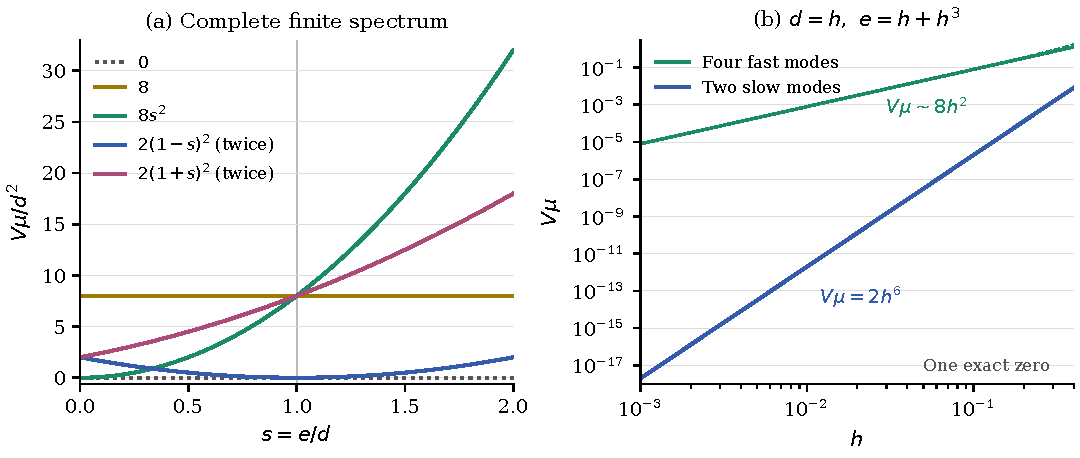
\includegraphics[width=\textwidth]{output/figures/two_cycle_spectrum.pdf}
 \caption{The exact finite spectrum in \eqref{eq:two-cycle-spectrum}.
 Panel (a) shows all seven eigenvalues, with the two double
 branches labelled. At $e=d>0$ the kernel has dimension three.
 Panel (b) takes $d=h$, $e=h+h^3$: two modes have scale
 $h^6$, four have scale $h^2$, and one is exactly zero.
 These are finite matrix calculations. The relative theorem
 transfers their asymptotics to the actual HYM linearization.}
 \label{fig:two-cycle}
\end{figure}

Figure~\ref{fig:two-cycle} also illustrates why the size
of the arrows alone does not determine the weakest rates.
The linear relaxation time of the two difference modes is
of order $h^{-2b}$. An approximation of nonlinear
trajectories on such intervals requires more than the
spectral comparison. The next three sections construct
the exact finite evolution and the phase selected by a
spatially varying initial metric.

\section{Heat smoothing and entry from spatial initial metrics}
\label{sec:spatial-entry}

Fix a smooth base point $p$ and an actual HE representative
$w$ from Proposition~\ref{prop:exact-balancing-coordinates}.
Throughout the flow argument these parameters remain fixed.
Write $r=|w|$, $D=D_{\mathcal A_p(w)}=D_0+a$ and
$L=D^*D$, $L_0=D_0^*D_0$. All section variables are
Hermitian and trace free for the fixed transported metric $h_0$.
Let $\Pi$ be the split projection onto $\mathfrak h$ and
$Q=I-\Pi$. On each smooth fibre put
\begin{equation}\label{eq:flow-banach-spaces}
 Y_p=C^0(\Herm_0E^{\rm sp}),\qquad
 X_p=C^1(\Herm_0E^{\rm sp}),\qquad
 \|u\|_X=\|u\|_\infty+\|D_0u\|_\infty.
\end{equation}
We use these fibrewise spaces with uniform operator bounds;
no fixed Banach bundle through the singular fibre is required.

\begin{theorem}\label{thm:spatial-entry}
There are $M,\sigma,C,\delta,r_0>0$, independent of the
base scales and of all positive weak-rate ratios, such that
\begin{equation}\label{eq:split-heat-smoothing}
 \begin{split}
 \|e^{-tL_0}Q\|_{X_p\to X_p}&\le Me^{-\sigma t},\\
 \|e^{-tL_0}Q\|_{Y_p\to X_p}
                    &\le M(1+t^{-1/2})e^{-\sigma t}\quad(t>0).
 \end{split}
\end{equation}
In the metric coordinate $h=h_0e^u$, the actual HYM equation is
\begin{equation}\label{eq:exact-log-flow}
                  \dot u+L_0u=N_w(u).
\end{equation}
Here $N_w:X_p\to Y_p$ depends only on the first spatial
jet, and is smooth with uniform derivatives of every fixed
finite order on a common small ball. For parallel $S$ and
$v\in QX_p$ with $|S|,\|v\|_X\le\delta_1$, it satisfies
\begin{equation}\label{eq:flow-nonlinearity-bounds}
 \begin{split}
 \|N_w(S)\|_\infty&\le Cr^2|S|,\\
 \|N_w(S+v)-N_w(S)\|_\infty&\le C(r+\delta_1)\|v\|_X.
 \end{split}
\end{equation}
Every fixed positive-order derivative of $N_w(S)$ in $S$
is $O(r^2)$ on this ball.

For every smooth $u_0$ with $\|u_0\|_X<\delta$ and
$r<r_0$, the determinant-normalized actual flow exists
for all $t\ge0$, stays in a common small $C^1$ ball, and obeys
\begin{equation}\label{eq:normal-entry}
 \begin{split}
 \|u(t)\|_\infty&\le\|u_0\|_\infty,
       \qquad |\Pi u(t)|\le\|u_0\|_\infty,\\
 \|Qu(t)\|_X&\le Ce^{-\sigma t/2}\|Qu_0\|_X
                         +Cr^2\|u_0\|_\infty.
 \end{split}
\end{equation}
For $0<r<\min(r_0,1)$, the time
$T_r=4\sigma^{-1}\log(1/r)$ gives $\|Qu(t)\|_X\le Cr^2\delta$
for all $t\ge T_r$. Every positive weak eigenvalue satisfies
$T_r\lambda_j\to0$ uniformly as $r\to0$.
\end{theorem}

\subsection{Uniform first derivatives of the split heat flow}

Let $S_t=e^{-tL_0}$ and let $H_t$ denote scalar heat flow.
Kato domination gives $|S_tf|\le H_t|f|$, so
$\|S_tf\|_\infty\le\|f\|_\infty$.
The scalar estimates from Section~\ref{sec:projected-he} and
Bochner's formula with $\operatorname{Ric}(g_p)=0$ give
\begin{equation}\label{eq:scalar-two-gradient-bounds}
 \|\dd H_t\phi\|_\infty\le Ct^{-1/2}\|\phi\|_\infty,
 \qquad
 \|\dd H_t\phi\|_\infty\le C\|\dd\phi\|_\infty.
\end{equation}
Use the fixed finite cover and unitary line frames from
the proof of Lemma~\ref{lem:graph-inverse}. Their connection
coefficients are bounded and divergence free. The partition
functions $\chi_j$ have uniformly bounded gradients and
Laplacians; the derivatives of the core cutoffs are supported
in fixed exterior annuli. If $f_j(t)$ is a scalar coefficient
of $S_tf$ in one frame, extend $z_j=\chi_jf_j$ by zero
to the whole fibre. The local formula
\eqref{eq:local-rough-operator} gives
\[
 (\partial_t+\Delta)z_j=F_j,
 \qquad \|F_j(t)\|_\infty
       \le C\{\|D_0S_tf\|_\infty+\|f\|_\infty\}.
\]
Conversely,
$\|D_0S_tf\|_\infty\le C\sum_j\|\dd z_j\|_\infty+C\|f\|_\infty$.
No derivative of the full curvature enters these formulas.

Scalar Duhamel and \eqref{eq:scalar-two-gradient-bounds}
therefore give, for $G(t)=\|D_0S_tf\|_\infty$ and
$F=\|f\|_\infty$,
\[
 G(t)\le C(t^{-1/2}+1)F+
      C\int_0^t(t-s)^{-1/2}\{G(s)+F\}\,\dd s
                       \quad(0<t\le1).
\]
For smooth $f$, set $Z_T=\sup_{0<t\le T}\sqrt t\,G(t)$.
The identity
$\int_0^t(t-s)^{-1/2}s^{-1/2}\,\dd s=\pi$
implies $Z_T\le CF+C\sqrt T Z_T$. One common small
$T$ absorbs the last term. The semigroup law extends the
bound to fixed bounded time intervals. For $f\in C^1$,
use the second scalar estimate on the initial term instead.
Taking $\sup_{0<t\le T}G(t)$ and using
$\int_0^t(t-s)^{-1/2}\,\dd s=2\sqrt t$ yields
\[
 \|S_tf\|_X\le C\|f\|_X\quad(0\le t\le1),\qquad
 \|S_tf\|_X\le C(1+t^{-1/2})\|f\|_\infty\quad(0<t\le1).
\]
Density extends these estimates. On each fixed smooth fibre,
the smooth heat solutions converge to their initial data in
$C^1$; density and the first estimate prove strong continuity
on $X_p$. The same argument works on $Y_p$.

The averaging projection $\Pi$ is uniformly bounded on both
spaces and commutes with $S_t$. The split $L^2$ gap, fixed
volume, and the fixed-time $L^2$-to-$L^\infty$ bound used in
Lemma~\ref{lem:graph-inverse} give
$\|S_tQ\|_{Y_p\to Y_p}\le Ce^{-ct}$ for $t\ge1$.
Composing with a fixed positive-time $Y_p$-to-$X_p$ map
proves \eqref{eq:split-heat-smoothing}. This argument supplies
the first-derivative smoothing needed below without a
uniform higher-order elliptic estimate.

\subsection{The contracted connection derivative}

The connection expansion already gives $\|a\|_\infty\le Cr$.
We also need its divergence:
\begin{equation}\label{eq:connection-divergence}
                         \|D_0^*a\|_\infty\le Cr^2.
\end{equation}
Indeed put $U=e^{s_p(w)/2}$ and
$\gamma=Ub_p(w)U^{-1}-(\dbar_0U)U^{-1}$, so $a=\gamma-\gamma^*$.
Section~\ref{sec:projected-he} gives
\[
 \|b_p(w)\|_\infty\le Cr,\quad
 \|\dbar_0^*b_p(w)\|_\infty\le Cr^2,
 \quad \|D_0U\|_\infty+\|P_pU\|_\infty\le Cr^2.
\]
The same first-derivative estimate holds for $U^{-1}$.
The divergence product rule gives
\[
 \begin{split}
 \dbar_0^*(UbU^{-1})
 &=U(\dbar_0^*b)U^{-1}
                  +O_\infty(|D_0U||b|+|b||D_0U^{-1}|),\\
 \dbar_0^*((\dbar_0U)U^{-1})
 &=(P_pU)U^{-1}+O_\infty(|D_0U||D_0U^{-1}|).
 \end{split}
\]
Thus $\|\dbar_0^*\gamma\|_\infty\le Cr^2$.
Real unitary divergence commutes with adjoints, proving
\eqref{eq:connection-divergence}.
For $A_j=\operatorname{ad}_{a(e_j)}$ in a real orthonormal
frame, expansion of the connection Laplacian gives
\begin{equation}\label{eq:rough-operator-perturbation}
 (L-L_0)u=-2\sum_j A_jD_{0,e_j}u+[D_0^*a,u]-\sum_jA_j^2u.
\end{equation}
Its first-order coefficient is $O(r)$ and its zeroth-order
coefficient is $O(r^2)$.

\subsection{The exact equation in logarithmic coordinates}

Define the pointwise invertible linear map
\[
 J_u(V)=\int_0^1e^{-\theta u}Ve^{\theta u}\,\dd\theta.
\]
It satisfies $e^{-u}(\dd\exp)_u(V)=J_u(V)$.
Diagonalization of $u$ shows that its scalar multipliers
are $(1-e^{-a})/a$, with value one at $a=0$.
Its inverse and all fixed-order derivatives are bounded
on a fixed small pointwise ball. Since the reference
connection $D$ is HE, the exact Chern formula is
\[
 \mathrm i\Lambda F_{h_0e^u}
 =\mathrm i\Lambda\dbar_D(J_u(D'_Du))
 =J_u(\mathrm i\Lambda\dbar_DD'_Du)
       +\mathrm i\Lambda(dJ)_u[\dbar_Du]\wedge D'_Du.
\]
The section Kähler identity gives
$\mathrm i\Lambda\dbar_DD'_Du=Lu/2$.
Consequently $h^{-1}\dot h=-2\mathrm i\Lambda F_h$ becomes
\begin{equation}\label{eq:first-jet-nonlinearity}
 \begin{split}
 \dot u+Lu&=\mathcal Q(u,Du),\\
 \mathcal Q(u,Du)&=-2J_u^{-1}\mathrm i\Lambda
                       (dJ)_u[\dbar_Du]\wedge D'_Du.
 \end{split}
\end{equation}
Here $dJ$ differentiates its finite matrix coefficient $u$.
The nonlinear term is quadratic in the first spatial jet;
all second derivatives have cancelled. Thus
\begin{equation}\label{eq:Nw-definition}
 N_w(u)=-(L-L_0)u+\mathcal Q(u,D_0u+[a,u])
\end{equation}
has the asserted uniform smoothness from $X_p$ to $Y_p$.
This follows from bounded matrix derivatives and the
continuous pointwise product $C^0\times C^0\to C^0$.
The equation preserves Hermitian variables by its metric
origin. It preserves trace zero because the determinant
metric solves scalar heat and initially equals the fixed
HE determinant.

For parallel $S$, the first-order term in
\eqref{eq:rough-operator-perturbation} vanishes, and
$DS=[a,S]$. Hence $N_w(S)=O(r^2|S|)+O(r^2|S|^2)$,
with the same factor $r^2$ in every fixed finite derivative.
Taking the difference at $S+v$ proves
\eqref{eq:flow-nonlinearity-bounds}.

\subsection{Confinement and normal decay}

On each fixed compact smooth fibre, global smooth HYM
metric flow from a smooth positive metric follows from
\cite[Theorem 6.8.25]{Kobayashi}. We use this only for existence;
its higher constants need not be uniform. The squared
pointwise distance from $h_0$ to $h_0e^u$ in the space
of positive Hermitian metrics is $\tr u^2$.
The two-solution distance inequality
\cite[Lemma 6.4.5]{Kobayashi}, with time changed by $\tau=2t$
to our convention, gives
\begin{equation}\label{eq:metric-distance-heat}
          (\partial_t+\Delta)\tfrac12\tr u^2\le0.
\end{equation}
The reference HE metric is stationary. The maximum principle
therefore proves the first bound in \eqref{eq:normal-entry}.
Block averaging and Jensen's inequality give the bound
for $S(t)=\Pi u(t)$.

Let $v=Qu$ and $\varepsilon=\|u_0\|_\infty$.
As long as $\|v\|_X\le\delta_1$, Duhamel gives
\begin{equation}\label{eq:normal-volterra}
 \|v(t)\|_X\le Me^{-\sigma t}\|v(0)\|_X+
  \int_0^t k(t-s)\{a_0\|v(s)\|_X+b_0\}\,\dd s,
\end{equation}
where $k(t)=M'(1+t^{-1/2})e^{-\sigma t}$,
$a_0=C(r+\delta_1)$, and $b_0=Cr^2\varepsilon$.
Choose $\delta_1,r_0$ so that
$a_0\int_0^\infty k(t)e^{\sigma t/2}\,\dd t\le1/2$.
Iteration of this nonnegative convolution inequality gives
\[
 \|v(t)\|_X\le2Me^{-\sigma t/2}\|v(0)\|_X
                              +2b_0\int_0^\infty k(s)\,\dd s.
\]
Equivalently the right side is a supersolution: its
exponential term is controlled by the weighted kernel
integral and its constant term by the unweighted integral.
Uniform boundedness of $\Pi,Q$ lets us choose one initial
$\delta$ making this bound smaller than $\delta_1/2$.
A first-exit argument then proves it for all time.
Since $D_0S=0$, this also confines $u$ in the required
$C^1$ ball and completes \eqref{eq:normal-entry}.

At $T_r$ the exponential is at most $r^2$.
Theorem~\ref{thm:complete-bundle-spectrum} gives
$\lambda_j\le Cr^2$ for every positive weak rate, so
$T_r\lambda_j\le Cr^2\log(1/r)\to0$.
This proves Theorem~\ref{thm:spatial-entry}, including
arbitrarily unequal weak rates. At $r=0$ there are no
positive weak rates, and the normal part decays exponentially.

The basin is an open ball in the $C^1$ topology intersected
with smooth determinant-normalized metrics. It contains
spatially varying initial metrics. The persistent $O(r^2)$
normal term in \eqref{eq:normal-entry} does not by itself
give tracking on a long time interval. We next absorb
that term into an invariant finite-dimensional graph.

\section{An invariant graph and its exact finite gradient flow}
\label{sec:invariant-dynamics}

The stationary metric correction of Section~\ref{sec:projected-he}
does not define an invariant graph for metric evolution. We
construct such a graph directly from the heat estimates of
Section~\ref{sec:spatial-entry}. Fix a finite regularity order
$m\ge4$. The constants and the chosen graph may depend on $m$.

\begin{theorem}\label{thm:invariant-graph}
After a common shrink there is a chosen $C^m$ map
$\psi_{p,w}:\mathfrak h\to QX_p$, with $\psi_{p,w}(0)=0$,
such that
\begin{equation}\label{eq:graph-derivative-bounds}
 \sup_S\|D_S^j\psi_{p,w}(S)\|_X\le C_mr^2
                          \quad(0\le j\le m).
\end{equation}
For $j\le m-1$ the same bound holds for
$L_0D_S^j\psi$ in $Y_p$. The graph is invariant for
the extension defined below and locally invariant for actual
HYM. Its complete finite field $f_{p,w}$ satisfies
$\|f_{p,w}\|_{C^m}\le C_mr^2$.
On a fixed inner ball, a trajectory of this field reconstructs
the actual metric flow
\begin{equation}\label{eq:graph-reconstruction}
             h(t)=h_0\exp\{S(t)+\psi_{p,w}(S(t))\}.
\end{equation}
The graph points there are spatially smooth on each fixed fibre.
At zero the tangent map $J_0=I+D\psi_{p,w}(0)$ identifies
$\mathfrak h$ with the complete seven-dimensional small
spectral space of $L$, and
\begin{equation}\label{eq:graph-linear-intertwining}
                         J_0Df_{p,w}(0)=-LJ_0.
\end{equation}
All exact kernel directions are retained.
The construction is jointly $K$-equivariant in $w$ and $S$.
\end{theorem}

\subsection{A smooth extension of the first-jet equation}

Choose smooth scalar cutoffs $\theta,\chi$ taking values in
$[0,1]$, equal to one on $[0,1]$ and zero on $[4,\infty)$.
For a fixed small $a>0$, put
\[
 \widehat S=\chi(|S|^2/a^2)S,\qquad
 \vartheta(v)(x)=\theta\bigl((|v(x)|^2+|D_0v(x)|^2)/a^2\bigr).
\]
The extended nonlinearity is
\begin{equation}\label{eq:jet-extension}
 \widetilde N_w(S,v)(x)=\vartheta(v)(x)
                                  N_w(\widehat S+v)(x).
\end{equation}
Its right side is evaluated using the pointwise formula
\eqref{eq:Nw-definition}, with $D_0\widehat S=0$.
Choose $a$ so that the support of the cutoff lies strictly
inside that formula's pointwise domain, and extend by zero
outside. This uses a smooth cutoff in finite-dimensional
first-jet variables. It requires no smooth bump function
of the $C^1$ norm.

The bounded jet map $v\mapsto(v,D_0v)$ and the pointwise
chain rule make $\widetilde N_w:\mathfrak h\times QX_p\to Y_p$
globally smooth and bounded, with uniform fixed-order
derivative bounds. On the cutoff support the drift term
has size $O(ra)$ and the quadratic term has size $O(a^2+r^2a^2)$.
A cutoff derivative contributes at most $C/a$.
For $r\le a$ this proves
\begin{equation}\label{eq:extended-small-lipschitz}
 \|D\widetilde N_w\|\le\ell=C(a+r),\qquad
 \sup_S\|D_S^j\widetilde N_w(S,0)\|_Y\le C_jr^2.
\end{equation}
The second bound follows because every occurrence of a
parallel variable in \eqref{eq:Nw-definition} retains two
connection factors or the zeroth-order coefficient.
Also $\widetilde N_w(0,0)=0$.
Set
$\mathcal A(S,v)=\Pi\widetilde N_w(S,v)$ and
$\mathcal B(S,v)=Q\widetilde N_w(S,v)$, absorbing the
uniform projection norms into $\ell$. The extended system is
\begin{equation}\label{eq:extended-system}
 \dot S=\mathcal A(S,v),\qquad
 \dot v=-L_0v+\mathcal B(S,v).
\end{equation}
It agrees with actual HYM when $|S|<a$ and $\|v\|_X<a$.
The integrable smoothing kernel and global Lipschitz bounds
give unique global forward mild solutions on each fibre.
All cutoffs use invariant norms, so the extension is
jointly equivariant under parallel unitary conjugation.

\subsection{Backward histories and finite differentiability}

Let $k(t)=M(1+t^{-1/2})e^{-\sigma t}$ and
$K_\beta=\int_0^\infty k(t)e^{\beta t}\,\dd t$ for
$0\le\beta<\sigma$. For continuous histories on $(-\infty,0]$
use the norm
\[
 \|(S,v)\|_\beta=
       \sup_{t\le0}e^{\beta t}(|S(t)|+\|v(t)\|_X).
\]
Put $\eta=\sigma/(2(m+2))$. Reduce $a$ and then $r_0$
so that
\begin{equation}\label{eq:history-contractions}
 \ell(\beta^{-1}+K_\beta)<\tfrac12
 \quad\bigl(\eta\le\beta\le(m+1)\eta\bigr),
 \qquad \ell K_0<\tfrac12.
\end{equation}
For any endpoint $S_0$, solve
\begin{equation}\label{eq:backward-fixed-point}
 \begin{aligned}
 S(t)&=S_0-\int_t^0\mathcal A(S(s),v(s))\,\dd s,\\
 v(t)&=\int_{-\infty}^t e^{-(t-s)L_0}
                               \mathcal B(S(s),v(s))\,\dd s.
 \end{aligned}
\end{equation}
The two Lipschitz bounds are $\ell/\beta$ and
$\ell K_\beta$. Boundedness of the nonlinearities shows
that the map sends each indicated history space into itself:
the finite output grows at most linearly backwards, and
the normal output is bounded. Continuity of the latter
in $X_p$ follows by splitting off a short terminal interval
and using integrability of $k$. Thus there is a unique
fixed history, identical in all these weighted spaces.
Its normal part satisfies
\[
 \sup_{t\le0}\|v(t)\|_X
 \le K_0\{Cr^2+\ell\sup_{t\le0}\|v(t)\|_X\}\le Cr^2.
\]
Define $\psi(S_0)=v(0)$. The zero history gives $\psi(0)=0$.

We record the differentiability argument to account for
products of growing histories. The first variation solves
the linearized fixed-point equation with initial term
$(\delta S_0,0)$. Its integral operator has norm below
$1/2$ in each weight. Differences of fixed histories are
$O(|\delta S_0|e^{-\eta t})$, so the quadratic Taylor
remainder is $O(|\delta S_0|^2e^{-2\eta t})$.
Inverting in the $2\eta$ space proves actual
differentiability. At order $j$, the inhomogeneous terms
have the form
\[
 D^q(\mathcal A,\mathcal B)(S,v)
                 [Z_{i_1},\ldots,Z_{i_q}],
 \qquad q\ge2,\quad i_1+\cdots+i_q=j,
\]
with each $i_k<j$. Their weights add to $j\eta$.
The same inverse works there, and Taylor's formula with
the next derivative in the spare weight $(j+1)\eta$
proves differentiability and continuity. All these weights
are below $\sigma$. Evaluation at zero proves $C^m$
regularity of $\psi$ with uniform derivative bounds.

For the sharper $r^2$ bound, bounded mixed derivatives,
the normal bound, and \eqref{eq:extended-small-lipschitz}
give $D_S^j(\mathcal A,\mathcal B)=O(r^2)$ along every
fixed history. In the first normal variation, the finite
coefficient is therefore $O(r^2)$ and the normal coefficient
is small; absorption makes that variation $O(r^2)$.
At higher orders, a term with only finite variations has
an $O(r^2)$ coefficient, while every other term contains
an $O(r^2)$ normal variation. Induction in the weighted
equations proves \eqref{eq:graph-derivative-bounds}.
Uniqueness also proves joint equivariance.

\subsection{Invariance, domains and linearization}

Shift a fixed history by a finite time, attaching the forward
mild solution when necessary. Its negative tail still has
bounded normal component and at most linear finite growth.
The shifted normal integral has no term at minus infinity.
It therefore solves \eqref{eq:backward-fixed-point} with
its new endpoint. Uniqueness gives $v(t)=\psi(S(t))$.
Thus the graph is invariant and its field is
\begin{equation}\label{eq:finite-field}
                       f(S)=\mathcal A(S,\psi(S)).
\end{equation}
The chain rule and the preceding estimates give
$\|f\|_{C^m}\le C_mr^2$. This bounded field has a
complete finite flow in both time directions.

On the graph the mild equation and differentiation in
$X_p$ imply the generator-domain identity
\begin{equation}\label{eq:graph-domain-identity}
             L_0\psi(S)=\mathcal B(S,\psi(S))-D\psi(S)f(S).
\end{equation}
Indeed divide the mild formula at time $t$ minus its
initial value by $t$ and let $t\downarrow0$ in $Y_p$.
Strong continuity makes the integral quotient converge
to $\mathcal B$ and the left derivative equal $D\psi f$.
This is the definition of the generator domain.
Differentiating the right side and using closedness of
$L_0$ gives the claimed domain bounds through order $m-1$.

On a fixed smooth fibre, ordinary elliptic regularity now
gives $\psi,D\psi\in W^{2,q}$ for every finite $q$,
then $C^{1,\alpha}$. Equation~\eqref{eq:graph-domain-identity}
gives $C^{2,\alpha}$ regularity. In an inner finite ball,
a short graph trajectory stays where the cutoffs are
inactive, hence is a classical solution of the original
first-jet equation. Interior fixed-fibre parabolic
regularity makes it spatially smooth. These higher
regularity statements have no asserted uniform constants.
They justify the actual reconstruction
\eqref{eq:graph-reconstruction}.

At the HE origin $DN_w(0)=-(L-L_0)$.
Differentiating invariance gives
\eqref{eq:graph-linear-intertwining}.
The seven-dimensional image of $J_0$ is invariant under
the self-adjoint $L$ and lies in its operator domain.
Its restriction is self-adjoint for the induced mass;
the bound on $Df(0)$ puts all its eigenvalues in $[0,Cr^2]$.
The complementary gap in Theorem~\ref{thm:complete-bundle-spectrum}
then identifies this image with the whole small spectral
space. Since $\Pi J_0=I$, its coordinates are exactly
those of the inverse restricted projection.

If $S$ is in the constant actual parallel kernel, then
$DS=0$ and $h_0e^S$ is HE. Its constant history gives
$\psi(S)=f(S)=0$ in the inner ball. Conversely a finite
equilibrium reconstructs an HE metric. Integrating the
squared-distance identity in the proof of
\cite[Lemma 6.4.5]{Kobayashi} along the fibrewise geodesic
between two stationary HE metrics forces their logarithmic
difference to be $D$-parallel. Theorem~\ref{thm:complete-bundle-spectrum}
identifies that difference with a constant element of
$\mathfrak h$. Thus the local equilibrium set is exactly
the actual parallel kernel ball. This completes the proof
of Theorem~\ref{thm:invariant-graph}.

\subsection{The finite metric, energy and full Hessian}

Put $Z(S)=S+\psi(S)$ and $Z_Sa=a+D\psi(S)a$.
The pullback of the invariant $L^2$ metric on positive
Hermitian metrics is
\begin{equation}\label{eq:finite-flow-metric}
 g_{{\rm fin},S}(a,b)=\int_{X_p}\tr
             \{J_{Z(S)}(Z_Sa)J_{Z(S)}(Z_Sb)\}\,\dd V_{g_p}.
\end{equation}
Although the factors need not be $h_0$-Hermitian, they
are Hermitian for the current metric, so this is positive.
On the small ball it is uniformly equivalent to the
$L^2$ trace pairing of $Z_Sa,Z_Sb$, hence to $M$ since
$\Pi Z_Sa=a$.
Define
\begin{equation}\label{eq:finite-donaldson-energy}
 \mathcal E_{\rm fin}(S)=
 2\int_0^1\!\int_{X_p}
       \tr\{\mathrm i\Lambda F_{h_0e^{tZ(S)}}Z(S)\}
                                      \,\dd V_{g_p}\,\dd t.
\end{equation}
This is twice Donaldson's functional relative to $h_0$.
Its first variation, with $\dd V=\omega^3/3!$, is
\cite[Section 6.3, equations (6.3.25)--(6.3.27)]{Kobayashi}
\[
 \dd\mathcal D_h(\dot h)=\int_{X_p}
                      \tr(\mathrm i\Lambda F_h\,h^{-1}\dot h)\,\dd V.
\]
On the inner region where the graph carries the actual HYM
equation, graph invariance and its coefficient $-2$ give
\begin{equation}\label{eq:exact-finite-gradient}
                f=-\operatorname{grad}_{g_{\rm fin}}\mathcal E_{\rm fin}.
\end{equation}
This metric describes variations of metrics on one fixed
holomorphic bundle. The harmonic metric on varying bundle
moduli will be constructed separately.

\begin{corollary}\label{cor:relative-finite-hessian}
At an HE parameter $w=\chi_p(z)$, the exact finite mass
and Hessian satisfy
\begin{equation}\label{eq:finite-mass-hessian}
 \begin{split}
 g_{{\rm fin},0}(S,T)
   &=M(S,T)+\langle D\psi(0)S,D\psi(0)T\rangle_2,\\
 |g_{{\rm fin},0}-M|&\le C|z|^4M,\\
 (1-C|z|)E_{p,z}&\le\operatorname{Hess}_0\mathcal E_{\rm fin}
                                             \le(1+C|z|)E_{p,z}.
 \end{split}
\end{equation}
In particular the Hessian has the exact kernel of $E_{p,z}$,
and its bilinear error is bounded by
$C|z|\sqrt{E_{p,z}(S)E_{p,z}(T)}$.
\end{corollary}

\begin{proof}
At the critical origin the exact forms are
$N(S,T)=\langle J_0S,J_0T\rangle_2$ and
$H(S,T)=\langle LJ_0S,J_0T\rangle_2$.
Orthogonality gives the mass formula and its $O(r^4)$ bound.
The lower bound in \eqref{eq:whole-bundle-form} gives
$H\ge(1-Cr)E_{p,w}$.
Their kernels agree because $J_0$ is the inverse of
$\Pi$ on the full small spectral space and the actual
kernel consists of the constant stabilizer directions.
On the quotient by that common kernel, let $\bar N,\bar M$
be the quotient masses (the infima over representatives).
They are relatively $1+O(r^4)$ equivalent.
The positive generalized eigenvalues of $(H,N)$ are exactly
the positive small eigenvalues of $L$. Therefore
\eqref{eq:seven-eigenvalues} gives
\[
 \frac{\det\bar H}{\det\bar E_{p,w}}
  =\frac{\prod_{\lambda_j>0}\lambda_j}
         {\prod_{\mu_j>0}\mu_j}
                           \frac{\det\bar N}{\det\bar M}
  =1+O(r).
\]
Every eigenvalue of $\bar E_{p,w}^{-1/2}\bar H
\bar E_{p,w}^{-1/2}$ is at least $1-Cr$, and their
product is $1+O(r)$. Since the dimension is at most seven,
each is at most $1+Cr$. If the quotient has dimension
zero the assertion is immediate. This proves the full
relative form comparison without a lower bound for a
positive weak rate.
Finally equivariance of $\chi_p$ gives
$\delta_wS=d\chi_p(z)\delta_zS$, with derivative
$I+O(|z|)$ in the uniformly positive arrow norm.
Hence $E_{p,w}=(1+O(|z|))E_{p,z}$ as forms, including
kernels. Polarization on the quotient proves the
bilinear estimate.
\end{proof}

The exact linear generator is $-g_{{\rm fin},0}^{-1}H$.
The relative Hessian statement does not replace the
nonlinear field \eqref{eq:finite-field} by its quadratic
approximation on arbitrarily long time intervals.

\section{The spatial phase and all-time metric comparison}
\label{sec:phase-tracking}

Fix one graph from Theorem~\ref{thm:invariant-graph}, and
write $\phi_t$ for its complete finite flow. The phase
of a general initial metric will be defined by removing
this finite evolution from its parallel component.

\begin{theorem}\label{thm:all-time-tracking}
There are common $r_0,\delta,c,C>0$ and a $C^1$ map
$\Gamma_{p,w}:B_{X_p}(\delta)\to\mathfrak h$, with
uniformly bounded first derivative, having the following
properties. For every smooth initial metric in this ball,
let $u(t)$ be the actual flow and put
\[
 S(t)=\Pi u(t),\qquad
 y(t)=Qu(t)-\psi(S(t)),\qquad D_*=\|y(0)\|_X.
\]
Then
\begin{equation}\label{eq:phase-definition}
 \begin{split}
 \Gamma(u_0)&=\lim_{T\to\infty}\phi_{-T}(S(T)),\\
 S_{\rm eff}(t)&=\phi_t(\Gamma(u_0)),\qquad
 u_{\rm eff}(t)=S_{\rm eff}(t)+\psi(S_{\rm eff}(t))
 \end{split}
\end{equation}
are defined for all $t\ge0$. The reconstructed metric
$h_{\rm eff}=h_0e^{u_{\rm eff}}$ is an actual HYM solution
on the same fixed holomorphic bundle, and
\begin{equation}\label{eq:tracking-bounds}
 \|y(t)\|_X+\|u(t)-u_{\rm eff}(t)\|_X\le CD_*e^{-ct}.
\end{equation}
The centered relative logarithm
\begin{equation}\label{eq:centered-logarithm}
 \zeta(t)=\log\{e^{-u_{\rm eff}(t)/2}e^{u(t)}e^{-u_{\rm eff}(t)/2}\}
\end{equation}
satisfies $\|\zeta(t)\|_X\le CD_*e^{-ct}$, and hence
\begin{equation}\label{eq:metric-order-tracking}
 e^{-CD_*e^{-ct}}h_{\rm eff}(t)
       \le h(t)\le e^{CD_*e^{-ct}}h_{\rm eff}(t).
\end{equation}
All constants are independent of the base scales,
stabilizer type, and ratios of positive weak rates.
One can take $c=\sigma/2$, so the error is at most
$Cr^2D_*$ after $T_r=4\sigma^{-1}\log(1/r)$.

The phase equals $S_0$ on graph data $S_0+\psi(S_0)$.
It is unique among complete finite trajectories that
track $S(t)$ at an exponential rate greater than
$L_f=\|Df\|_\infty\le Cr^2$. It is jointly $K$-equivariant
and depends on the chosen graph and the full initial metric.
\end{theorem}

\subsection{Normal decay and the phase limit}

In the coordinates $S,y$, the extended equation is exactly
\begin{equation}\label{eq:normal-graph-equations}
 \dot S=f(S)+h(S,y),\qquad \dot y=-L_0y+F(S,y),
\end{equation}
where
\[
 \begin{split}
 h(S,y)&=\mathcal A(S,\psi(S)+y)-\mathcal A(S,\psi(S)),\\
 F(S,y)&=\mathcal B(S,\psi(S)+y)-\mathcal B(S,\psi(S))
                                                -D\psi(S)h(S,y).
 \end{split}
\]
The final term follows from differentiating the graph
coordinate and is essential. These maps vanish at $y=0$.
Their uniform derivatives satisfy
\begin{equation}\label{eq:normal-coupling-bounds}
 \|D_yh\|+\|D_yF\|\le\varepsilon,
 \qquad
 \|D_Sh(S,y)\|+\|D_SF(S,y)\|\le C\|y\|_X,
\end{equation}
where $\varepsilon$ is made small by choosing the cutoff
radius and then $r_0$. The second bound follows from
bounded mixed derivatives and vanishing at $y=0$.
For either sign of $t$, the finite variational equations give
\begin{equation}\label{eq:finite-backflow-bounds}
 \|D\phi_t\|\le e^{L_f|t|},\qquad
 \|D^2\phi_t\|\le K_f|t|e^{2L_f|t|},
 \qquad K_f=\|D^2f\|_\infty=O(r^2).
\end{equation}

Set $c=\sigma/2$. Choose the constants so that
$\varepsilon\int_0^\infty k(t)e^{ct}\,\dd t<1/2$.
The normal Duhamel formula then gives
\[
 \sup_{s\le T}e^{cs}\|y(s)\|_X
 \le MD_*+\tfrac12\sup_{s\le T}e^{cs}\|y(s)\|_X.
\]
It follows that $\|y(t)\|_X\le2MD_*e^{-ct}$.
This prevents normal exit for small initial $D_*$;
the bounded finite field and the integrable perturbation
$h$ prevent finite-time escape of $S$.

For $P_T=\phi_{-T}(S(T))$, differentiation cancels the
finite $f$ terms and gives
\begin{equation}\label{eq:phase-velocity}
        \frac{\dd P_T}{\dd T}
             =D\phi_{-T}(S(T))h(S(T),y(T)).
\end{equation}
Its norm is at most $C\varepsilon D_*e^{-(c-L_f)T}$.
Taking $L_f<c$ proves the phase limit and
$|\Gamma-S(0)|\le C\varepsilon D_*$.
For fixed $t$, apply the same differentiation to
$\phi_{t-T}(S(T))$ for $T\ge t$. Integration to infinity
gives
\begin{equation}\label{eq:finite-coordinate-tracking}
              |S(t)-S_{\rm eff}(t)|\le C\varepsilon D_*e^{-ct}.
\end{equation}
Together with the normal decay and $D\psi=O(r^2)$
this proves \eqref{eq:tracking-bounds} for the extended
system. If two finite trajectories track at rates larger
than $L_f$, applying $\phi_{-t}$ to their difference
forces their initial points to agree. Graph data have
$y=0$, so their phase is their initial finite coordinate.
This argument uses an upper expansion bound $L_f$;
it never divides by a positive weak rate.

\subsection{Differentiability of the phase}

The integrable smoothing kernel gives differentiable
dependence of mild solutions on each finite interval.
Let $W=\delta S$ and $Z=\delta y$. Their equations are
\[
 \begin{split}
 \dot W&=(Df+D_Sh)W+D_yh\,Z,\\
 Z(t)&=e^{-tL_0}Z(0)+\int_0^te^{-(t-s)L_0}
                     (D_SF\,W+D_yF\,Z)(s)\,\dd s.
 \end{split}
\]
Put $\gamma=\sigma/16$ and reduce $r_0$ so that
$L_f<\gamma/4$. With
$U_T=\sup_{t\le T}e^{-\gamma t}|W(t)|$ and
$V_T=\sup_{t\le T}e^{(c-\gamma)t}\|Z(t)\|_X$,
normal convolution and \eqref{eq:normal-coupling-bounds}
give
\[
 V_T\le C\|Z(0)\|_X+CD_*U_T,
 \qquad U_T\le C|W(0)|+C\varepsilon V_T.
\]
In the second inequality the coefficient $D_Sh$ is
integrable in time. For sufficiently small $D_*$,
absorption gives
\begin{equation}\label{eq:phase-variation-bounds}
 \begin{split}
 |W(t)|&\le Ce^{\gamma t}(|W(0)|+\varepsilon\|Z(0)\|_X),\\
 \|Z(t)\|_X&\le Ce^{-(c-\gamma)t}
                            (\|Z(0)\|_X+D_*|W(0)|).
 \end{split}
\end{equation}
The derivative of the velocity \eqref{eq:phase-velocity} is
\[
 D^2\phi_{-T}(S(T))[W(T),h]
      +D\phi_{-T}(S(T))(D_Sh\,W(T)+D_yh\,Z(T)).
\]
Its operator norm is bounded by a constant times
\[
 \varepsilon D_*(1+T)e^{-(c-2L_f-\gamma)T}
              +(D_*+\varepsilon)e^{-(c-L_f-\gamma)T}.
\]
This is uniformly integrable on a smaller initial ball.
The integral formula for $P_T$ therefore converges in
$C^1$, with continuous derivative by dominated convergence.
Composing with $S(0)=\Pi u_0$ and
$y(0)=Qu_0-\psi(\Pi u_0)$ proves the asserted phase
regularity. Equivariance follows from that of the
equations and uniqueness of the phase.

\subsection{Confinement in the actual equation}

Theorem~\ref{thm:spatial-entry} lets us reduce $\delta$
so that every smooth actual solution in the initial ball
satisfies $|S(t)|<a/4$ and $\|Qu(t)\|_X<a/4$ for all
positive time. Thus it remains where the extended and
actual equations agree. Local mild uniqueness identifies
the two solutions globally. Also
$D_*\le\|Qu_0\|_X+Cr^2|\Pi u_0|\le C\delta$.
Reduce $\delta$ again so that
\eqref{eq:finite-coordinate-tracking} is less than $a/4$.
Then $|S_{\rm eff}(t)|<a/2$, and the graph bound gives
$\|\psi(S_{\rm eff}(t))\|_X<a/4$. The selected graph
trajectory also stays in the actual region for all time.
Theorem~\ref{thm:invariant-graph} reconstructs its spatially
smooth actual HYM metric there.

The norm $X_p$ is a Banach algebra norm, since $D_0$ is
a derivation. Exponential and logarithm on a fixed small
positive matrix ball have bounded derivatives. Hence
\[
 (u,\widetilde u)\longmapsto
             \log(e^{-\widetilde u/2}e^ue^{-\widetilde u/2})
\]
is uniformly locally Lipschitz from $X_p\times X_p$ to
$X_p$ and vanishes on the diagonal. This proves the
bound for \eqref{eq:centered-logarithm}. Its matrix is
positive Hermitian with determinant one, so its spectral
bounds imply \eqref{eq:metric-order-tracking}. These
metric inequalities transport invariantly back to the
actual holomorphic bundle. The stated $C^1$ norm is the
one in the fixed transport used throughout the construction.
At $T_r$ we have $e^{-cT_r}=r^2$. This completes the
proof of Theorem~\ref{thm:all-time-tracking}.

\subsection{Finite preparation and all weak time scales}

The limit defining the phase has a finite preparation rule.
For any $T\ge0$, put $\Gamma_T=\phi_{-T}(\Pi u(T))$
and let $u_{{\rm eff},T}$ be the graph trajectory starting
at $\Gamma_T$. Integrating \eqref{eq:phase-velocity} gives
\begin{equation}\label{eq:finite-phase-error}
 |\Gamma_T-\Gamma|\le C\varepsilon D_*e^{-(c-L_f)T},
 \qquad |\Gamma_T-S(0)|\le C\varepsilon D_*.
\end{equation}
All these initial points can be put in a common graph
ball whose positive trajectories are actual and confined:
for small $S_1$, $\|S_1+\psi(S_1)\|_X\le C|S_1|$,
so Theorem~\ref{thm:spatial-entry} applies, and uniqueness
preserves the graph. A smaller initial $\delta$ puts
$\Gamma$ and every $\Gamma_T$ in that ball.

The two-solution distance inequality
\cite[Lemma 6.4.5]{Kobayashi}, applied to these two actual
graph flows, implies
\[
 \sup_x d_x(h_{{\rm eff},T}(t),h_{\rm eff}(t))
          \le\sup_x d_x(h_{{\rm eff},T}(0),h_{\rm eff}(0))
          \le C|\Gamma_T-\Gamma|.
\]
Here $d_x$ is the invariant distance on positive Hermitian
metrics in the fibre. On the common small ball it is
equivalent to the pointwise difference in logarithmic
coordinates. Apply the bounded projection $\Pi$ to
obtain $|S_T(t)-S_{\rm eff}(t)|\le C|\Gamma_T-\Gamma|$.
The graph derivative bound upgrades this finite-coordinate
bound to
\begin{equation}\label{eq:prepared-trajectory-error}
 \sup_{t\ge0}\|u_{{\rm eff},T}(t)-u_{\rm eff}(t)\|_X
                      \le C\varepsilon D_*e^{-(c-L_f)T}.
\end{equation}
The upgrade uses the finite graph; it does not assert
$C^1$ contraction for arbitrary metric flows.
Combining with the actual tracking estimate gives
\[
 \left\|\log\{e^{-u_{{\rm eff},T}(t)/2}e^{u(t)}
                           e^{-u_{{\rm eff},T}(t)/2}\}\right\|_X
       \le CD_*e^{-ct}+C\varepsilon D_*e^{-(c-L_f)T}.
\]
Since $L_f=O(r^2)$, taking $T=T_r$ makes the second
term $O(r^2D_*)$ uniformly for every later comparison time.
Moreover $T_r\lambda_j\to0$ for every positive weak rate.
Thus the preparation is negligible compared with all
inverse weak rates, including the times $h^{-2b}$ in
Proposition~\ref{prop:two-cycle-spectrum}.

The comparison is absolute tracking to the exact corrected
field $f$. It does not supply a relative error divided by
a vanishing trajectory or a nonlinear asymptotic exponent.
The initial phase retains spatial information and is
generally different from $\Pi u_0$. After shrinking the
initial basin so that its evolved points remain in the
phase domain, uniqueness also gives
$\Gamma(u(t))=\phi_t\Gamma(u_0)$.
Nonpolystable escape to a graded boundary is outside this
metric basin around an HE representative.

\section{The harmonic quotient metric and unitary rigidity}
\label{sec:harmonic-quotient}

We now vary the holomorphic bundle, while keeping the smooth
base fibre fixed. The resulting harmonic metric has a different
domain from the metric in \eqref{eq:finite-flow-metric}.
For a skew-Hermitian connection one-form use
$\|a\|_2^2=-\int\tr(a\wedge *a)$, with volume $\omega_p^3/3!$.
On the matrix space $W=\operatorname{Mat}_2\oplus\operatorname{Mat}_2$
put
\begin{equation}\label{eq:flat-arrow-metric}
 G_{0,p}(q,q)=2c_+(p)\|q_A\|_{\rm HS}^2
                                  +2c_-(p)\|q_B\|_{\rm HS}^2.
\end{equation}
Let $\mathfrak k_0=\mathrm i\mathfrak h$ and let $Q$ also
denote the split complementary projection on skew-Hermitian
trace-free sections. The fundamental vector for the compact
action is
\[
 \rho_w\xi=(\xi_+A-A\xi_-,\ \xi_-B-B\xi_+).
\]
Exact equivariance of the actual connection map gives
\begin{equation}\label{eq:actual-gauge-action}
       d\mathcal A_p(w)(\rho_w\xi)=-D_{\mathcal A_p(w)}\xi.
\end{equation}
The ineffective scalar may equivalently be included in the
finite gauge algebra.

\begin{theorem}\label{thm:harmonic-quotient}
Uniformly in the base and every small $w$, for all $q\in W$
and $v\in QH^1(\mathfrak{su}E^{\rm sp})$,
\begin{equation}\label{eq:all-gauge-competitors}
 \begin{split}
 (1-C|w|)\{G_{0,p}(q,q)+\|D_0v\|_2^2\}
 &\le\|d\mathcal A_p(w)q-D_{\mathcal A_p(w)}v\|_2^2\\
 &\le(1+C|w|)\{G_{0,p}(q,q)+\|D_0v\|_2^2\}.
 \end{split}
\end{equation}
Consequently the full unitary-gauge minimum is relatively
equivalent, with error $O(|w|)$, to
\begin{equation}\label{eq:finite-quotient-metric}
             g^{\rm quot}_{0,p,w}(q)
                    =\inf_{\xi\in\mathfrak k_0}G_{0,p}(q-\rho_w\xi,q-\rho_w\xi).
\end{equation}
Its kernel is exactly $\im\rho_w$.
For $F_p(z)=\mathcal A_p(\chi_p(z))$ and genuine tangents
to a smooth orbit-type stratum of $\mu_{2,p}^{-1}(0)$,
the actual harmonic connection metric satisfies
\begin{equation}\label{eq:harmonic-relative-metric}
 (1-C|z|)g^{\rm quot}_{0,p,z}
       \le F_p^*g_{\rm harm}\le(1+C|z|)g^{\rm quot}_{0,p,z}.
\end{equation}
This real metric is twice the Dolbeault harmonic
Kodaira--Spencer metric. The estimates allow every change
of stabilizer and all positive singular-value ratios of
$\rho_z$.
\end{theorem}

\begin{proof}
Split harmonicity and type orthogonality give
\[
 \|a_{1,p}(q)\|_2^2=2\|\eta_p(q)\|_2^2=G_{0,p}(q,q),
 \qquad \langle a_{1,p}(q),D_0v\rangle_2=0.
\]
The connection expansion \eqref{eq:connection-expansion}
and the split section gap imply
\[
 \begin{split}
 \|d\mathcal A_p(w)q-D_{\mathcal A_p(w)}v
                           -(a_{1,p}(q)-D_0v)\|_2
 &\le\|d\mathcal N_p(w)q\|_2+\|[a_p(w),v]\|_2\\
 &\le C|w|\{G_{0,p}(q,q)+\|D_0v\|_2^2\}^{1/2}.
 \end{split}
\]
Squaring proves \eqref{eq:all-gauge-competitors}; density
extends it to the stated $H^1$ domain. The minimum over
$QH^1$ exists uniquely by coercivity. Infimizing the lower
bound and taking $v=0$ for the upper bound gives a relative
comparison with $G_{0,p}(q,q)$.

Every full gauge direction is $\xi+v$. By
\eqref{eq:actual-gauge-action}, its residual is
$d\mathcal A_p(w)(q+\rho_w\xi)-D_{\mathcal A_p(w)}v$.
Apply the preceding comparison to every $q+\rho_w\xi$
and then infimize in $\xi$. Changing its sign gives
\eqref{eq:finite-quotient-metric}. The finite range is
closed at each parameter, so the kernel is precisely
$\im\rho_w$. No estimate for the size of a minimizing
$\xi$ has been used.

Real equivariance gives
$d\chi_p(z)\rho_z\xi=\rho_{\chi_p(z)}\xi$.
Since $d\chi_p=I+O(|z|)$ in the uniformly positive arrow
metric, the same comparison transfers through $\chi_p$
inside every residual before minimization. This proves
\eqref{eq:harmonic-relative-metric} as a quotient form.

For its harmonic interpretation, take a smooth curve in
one zero-level orbit-type stratum. Its actual derivative
$a$ at the HE connection $D_A$ satisfies
$(D_Aa)^{0,2}=0$ and $\mathrm i\Lambda D_Aa=0$.
The full gauge minimum supplies the Coulomb representative
$a_h=a-D_A\zeta$, with $D_A^*a_h=0$.
Subtracting this vertical preserves the two linearized
equations because $F_A^{0,2}=0$ and
$\mathrm i\Lambda F_A=0$. The Kähler identities identify
the Coulomb and contracted equations with the sum and
difference of the two adjoint expressions, giving
\[
 \dbar_A(a_h^{0,1})=0,\qquad \dbar_A^*(a_h^{0,1})=0.
\]
This is the harmonic representative of the actual
Kodaira--Spencer class; a unitary vertical is a Dolbeault
coboundary. Type orthogonality gives the factor two in
its real norm, in agreement with
\cite[Section 7.2 and equations (7.6.5), (7.6.20)--(7.6.21)]{Kobayashi}.
The orbit-type pieces of the zero level and their quotients
by $K$ are smooth by \cite[Theorem 2.1]{SL}.
The form is positive on their quotient tangents by its
identified kernel. For fixed $p$ it is smooth on each
stratum, by the elliptic inverse on the complement of
the constant-dimensional parallel kernel. No uniform
derivative across strata or through the singular base
is asserted.
\end{proof}

The same action occurs in the weak endomorphism energy:
\begin{equation}\label{eq:shared-action-energy}
             E_{p,z}(S)=G_{0,p}(\rho_z(\mathrm iS),\rho_z(\mathrm iS)).
\end{equation}
Thus its kernel is the infinitesimal stabilizer, while
the null directions of the quotient tangent metric are
the image of the action. These are different spaces
related by one specified map.

\subsection{All unitary intertwiners are constant}

An infinitesimal metric comparison does not identify
different finite quotient points with different bundle
classes. The following statement supplies that identification.

\begin{theorem}\label{thm:unitary-rigidity}
On a common small parameter ball, every unitary gauge
transformation intertwining $\mathcal A_p(w_1)$ and
$\mathcal A_p(w_2)$ is a split parallel block unitary
$K\in U(2)\times U(2)$, and $w_2=K\cdot w_1$.
At HE points, two constructed holomorphic bundles are
isomorphic if and only if their parameters lie in the
same $K$-orbit. The same assertion holds in the balanced
$z$ coordinates.
\end{theorem}

\begin{proof}
Put $\rho=\max(|w_1|,|w_2|)$ and abbreviate the connection
increments by $a_j=a_p(w_j)$. The intertwining equation gives
\[
 D_0k=ka_1-a_2k,\qquad \|D_0k\|_\infty\le C\rho.
\]
Equation~\eqref{eq:connection-divergence} holds for every
small slice parameter: its proof did not use the HE equation.
Taking divergence therefore gives
\[
 L_0k=kD_0^*a_1-(D_0^*a_2)k
       -\sum_j(D_{0,e_j}k)a_1(e_j)
       +\sum_ja_2(e_j)D_{0,e_j}k=O_\infty(\rho^2).
\]
Let $\widehat\Pi$ project onto the full complex split
parallel algebra $\operatorname{Mat}_2\oplus\operatorname{Mat}_2$.
The full complex inverse in Lemma~\ref{lem:graph-inverse}
implies
\begin{equation}\label{eq:intertwiner-complement}
                    \|k-\widehat\Pi k\|_{C^1(D_0)}\le C\rho^2.
\end{equation}
Since $k$ is unitary, $B=\widehat\Pi k$ satisfies
$B^*B=I+O(\rho^2)$. Its block polar factor $K_0$
is unitary and $\|K_0^{-1}k-I\|_{C^1(D_0)}\le C\rho^2$.
In the finite skew-Hermitian block algebra solve
\[
                 \widehat\Pi\log(e^{-C}K_0^{-1}k)=0.
\]
The derivative in $C$ at the identity is $-I$ and differs
from it by $O(\rho^2)$ for these data. A uniform finite
contraction gives $|C|\le C\rho^2$. Thus
\begin{equation}\label{eq:intertwiner-factorization}
 k=Ke^\xi,\qquad K=K_0e^C\in K,\qquad
 \widehat\Pi\xi=0,\qquad \|\xi\|_{C^1(D_0)}\le C\rho^2.
\end{equation}
The determinant connection is fixed, so $\det k$ is
constant. The small logarithm makes $\tr\xi$ constant,
and its zero parallel projection makes this trace zero.

Conjugate the second connection by $K^{-1}$ and put
$\delta=K^{-1}\cdot w_2-w_1$. The segment between these
two parameters stays in the small slice, giving
\[
 a(K^{-1}\cdot w_2)-a(w_1)=a_{1,p}(\delta)+R_\delta,
                         \qquad \|R_\delta\|_2\le C\rho|\delta|.
\]
The exact exponential gauge identity is
\[
 e^\xi D(w_1)e^{-\xi}-D(w_1)
                 =-\int_0^1e^{t\xi}(D(w_1)\xi)e^{-t\xi}\,\dd t.
\]
The split gap on $\widehat\Pi^\perp$, together with
\eqref{eq:intertwiner-factorization}, therefore gives
\[
 \|a_{1,p}(\delta)+D_0\xi\|_2
                         \le C\rho(|\delta|+\|D_0\xi\|_2).
\]
The two terms on the left are orthogonal, and their
squared norm is
$G_{0,p}(\delta,\delta)+\|D_0\xi\|_2^2$.
The uniform positive arrow masses allow absorption for
small $\rho$. Hence $\delta=0$, $D_0\xi=0$, and then
$\xi=0$. Every intertwiner is the constant $K$.

For a holomorphic isomorphism $T$ between two HE members,
the induced Hom connection has zero mean curvature.
Its section Kähler identity gives
$\|D_{\rm Hom}T\|_2^2=2\|\dbar_{\rm Hom}T\|_2^2=0$;
see also \cite[Theorem 3.1.9(i)]{Kobayashi}.
Thus $T$ and its positive polar factor are parallel,
and its unitary polar factor is an intertwiner.
The first assertion applies, without simplicity or
stability assumptions. The converse is equivariance.
Finally injectivity and equivariance of $\chi_p$ transfer
the assertion to balanced parameters.
\end{proof}

\subsection{The topology of the actual local locus}

On a fixed smooth fibre take the affine space of continuous
unitary connections, with its $C^0$ topology, modulo $C^1$
unitary gauge. This quotient is Hausdorff. Indeed, suppose
$D_{j,n}\to D_j$ and $D_{2,n}=k_nD_{1,n}k_n^{-1}$.
The intertwiners are pointwise unitary and
\[
 D_0k_n=k_n(D_{1,n}-D_0)-(D_{2,n}-D_0)k_n.
\]
Their first derivatives are bounded on this fixed compact
manifold. Arzelà--Ascoli gives a uniformly convergent
subsequence; the equation then gives convergence of the
first derivatives and a $C^1$ unitary intertwiner in the
limit. Hence the orbit relation is closed. The orbit
projection is open because saturations are unions of
translates, so the quotient is Hausdorff. For smooth
endpoints the displayed equation bootstraps an intertwiner
to smoothness, introducing no extra identifications.

For any compact invariant subset of the balanced zero
set, Theorem~\ref{thm:unitary-rigidity} makes its quotient
map into actual connection classes continuous and
injective. A compact-to-Hausdorff injection is a
homeomorphism onto its image. These points are precisely
distinct actual holomorphic bundle classes.
The local completeness proved in Section~\ref{sec:balancing}
shows that a nested such locus contains representatives
of every sufficiently small polystable object in the
specified local germ. This is the germ coverage already
proved there; $\chi_p$ is a real parametrization and
does not supply a holomorphic chart or an algebraic
Cartesian square of moduli spaces.

\section{Local distance, completion and the metric tangent cone}
\label{sec:metric-cone}

Normalize the arrows by $T_p(A,B)=(\sqrt{c_+}A,\sqrt{c_-}B)$.
The balanced set is
\[
 \mathcal Z=\{(X,Y):XX^*=Y^*Y,\ YY^*=X^*X\},
\]
with real metric $2(\|\dd X\|_{\rm HS}^2+\|\dd Y\|_{\rm HS}^2)$.
Let $\mathsf W=(\ZZ/2)^2\rtimes S_2$ act on $\CC^2$
by independent signs and permutation. For
$u=(u_1,u_2)$ and $U=\diag(u_1,u_2)$, define
\begin{equation}\label{eq:actual-moduli-parametrization}
 \mathfrak F_p([u])=
       [\mathcal A_p(\chi_p(T_p^{-1}(U,U)))].
\end{equation}
The brackets on the right denote actual unitary gauge
classes, equivalently actual holomorphic bundle classes
at these HE points.
Choose one $R_0>0$ so that $|u|\le R_0$ lies strictly
inside every construction domain, uniformly in $p$.
Put $\mathcal M_p(R)=\mathfrak F_p(\overline B_R/\mathsf W)$
for $0<R\le R_0$.

An admissible path in this locus is continuous and has
a finite subdivision into smooth paths in its quotient
orbit-type strata, with improper endpoint lengths allowed.
Its length is the integral of the actual harmonic
connection norm of its bundle-deformation tangent.
Let $d_{p,R}$ be the infimum of these lengths among
paths confined to $\mathcal M_p(R)$.

\begin{theorem}\label{thm:metric-cone}
The map \eqref{eq:actual-moduli-parametrization} is a
homeomorphism of $\overline B_R/\mathsf W$ onto its
actual image, with smooth image-stratum parametrizations.
On every stratum its harmonic metric satisfies
\begin{equation}\label{eq:diagonal-harmonic-metric}
       (1-C|u|)\,4|\dd u|^2
       \le\mathfrak F_p^*g_{\rm harm}\le(1+C|u|)\,4|\dd u|^2.
\end{equation}
For $|u|,|v|\le R$, set
$d_{\rm flat}([u],[v])=2\min_{\gamma\in\mathsf W}|u-\gamma v|$.
Then
\begin{equation}\label{eq:confined-distance-comparison}
 \sqrt{1-CR}\,d_{\rm flat}([u],[v])
 \le d_{p,R}(\mathfrak F_p[u],\mathfrak F_p[v])
 \le\sqrt{1+CR}\,d_{\rm flat}([u],[v]).
\end{equation}
The open-radius locus completes isometrically to this
closed-radius locus. On the unit quotient ball,
\begin{equation}\label{eq:rescaled-distance}
 \sup_{[u],[v]}
 \left|\rho^{-1}d_{p,\rho}(\mathfrak F_p[\rho u],\mathfrak F_p[\rho v])
                          -d_{\rm flat}([u],[v])\right|\le C\rho.
\end{equation}
The same estimate holds with the single fixed-locus
distance $d_{p,R_0}$ for $\rho<R_0/8$.
The actual local metric space therefore has the unique
pointed metric tangent cone
\begin{equation}\label{eq:moduli-cone}
                         (\CC^2,4|\dd u|^2)/\mathsf W
\end{equation}
at the split bundle. These comparisons and the resulting
Gromov--Hausdorff convergence are uniform over the smooth
conifold base, including simultaneous approaches to its
discriminant. The distances use paths in the specified
local locus.
\end{theorem}

\subsection{The exact finite quotient}

The balanced normal form in Section~\ref{sec:balancing}
is $X=\diag(d_j)$, $Y=\diag(d_je^{\mathrm i\theta_j})$.
Choose $u_j=d_je^{\mathrm i\theta_j/2}$.
Acting by $k_+=\diag(e^{\mathrm i\theta_j/2})$, $k_-=I$
makes both arrows equal $U$. The phase at a zero entry
is immaterial. Under the compact action $XY$ changes by
conjugation. For $(U,U)$ its eigenvalue multiset is
$\{u_1^2,u_2^2\}$. Thus two section points can be
equivalent only if they differ by $\mathsf W$.
Conversely permutations are realized simultaneously in
both blocks, and each sign change by a diagonal sign
in the plus block alone. This proves the quotient
identification, including repeated and zero entries.
On a closed radius ball it is a homeomorphism by
compactness, since
$\|X\|_{\rm HS}^2+\|Y\|_{\rm HS}^2=2|u|^2$ and
the compact group quotient is Hausdorff.

The four strata are distinct nonzero squares, repeated
nonzero squares, one zero square, and the origin.
Their preimages are the complement of the four complex
reflecting hyperplanes, the nonzero parts of $u_1=\pm u_2$,
the nonzero parts of the coordinate axes, and the origin.
They agree with the actual factor and stabilizer types.

The section also gives smooth local coordinates on each
stratum. On the balanced set $XY$ is normal and
$XX^*=|XY|$, since
$(XY)(XY)^*=(XX^*)^2=(XY)^*(XY)$.
For distinct eigenvalues its spectral projections vary
smoothly. For a nonzero eigenvalue $\lambda$, choose a
smooth local square root $u$ and a smooth unit eigenvector
$e_+$; then $e_-=X^*e_+/\bar u$ is unit and satisfies
$Xe_-=ue_+$, $Ye_+=ue_-$.
At a simple zero eigenvalue use smooth frames of the
kernels, on which both arrows vanish. On the repeated
nonzero stratum $XY=\lambda I$ and the same formula
works with an arbitrary smooth plus frame. These are
qualitative coordinates within a stratum; no uniform
bound for their derivatives near another stratum is used.

For a diagonal section tangent $(V,V)$ the ambient norm
is $4\|V\|_{\rm HS}^2$. Its pairing with a vertical is
\[
 2\operatorname{Re}\tr
       V^*(\xi_+U-U\xi_-+\xi_-U-U\xi_+)
   =2\operatorname{Re}\tr V^*[\xi_++\xi_-,U]=0.
\]
Thus these tangents are horizontal, and the stratum
coordinates just proved exhaust the quotient tangents.
The exact finite quotient metric is $4\sum_j|\dd u_j|^2$.
On the repeated stratum it is $8|\dd u|^2$, and on
the one-nonzero stratum it is $4|\dd u|^2$; the origin
has zero stratum tangent.

Its path distance on a closed ball is $d_{\rm flat}$.
Local lifts of stratum paths and the triangle inequality
give the lower bound. For the upper bound choose a
minimizing $\gamma$ and project the straight segment
from $u$ to $\gamma v$. Convexity keeps it in the ball.
Each reflecting hyperplane meets the segment at at most
one parameter unless it contains the segment; a finite
subdivision therefore makes the projected segment
admissible. Its length attains the stated lower bound.

\subsection{Actual harmonic lengths and completion}

Theorem~\ref{thm:unitary-rigidity} and the compact quotient
argument of Section~\ref{sec:harmonic-quotient} identify
the finite quotient homeomorphically with actual classes.
Each image stratum is represented by a smooth family
of integrable HE connections. Its harmonic tangent
has no kernel beyond the compact vertical directions
by Theorem~\ref{thm:harmonic-quotient}.
Since $|T_p^{-1}(U,U)|\le C|u|$, that theorem and the
exact horizontal metric prove
\eqref{eq:diagonal-harmonic-metric}.
Integrating it over any admissible path gives the lower
bound in \eqref{eq:confined-distance-comparison}; using
the projected straight segment gives the upper bound.
In particular this is a finite nondegenerate distance
with exactly the compact quotient topology.

For interior endpoints the open-locus path distance
equals the restriction of the closed-locus distance.
One inequality is immediate. For the other, contract
any finite-length closed-locus path by $u\mapsto(1-\epsilon)u$.
The contracted pieces remain in their strata. The actual
tensor is smooth there, so their speeds converge pointwise.
Equation~\eqref{eq:diagonal-harmonic-metric} dominates
them by a constant times the original Euclidean speed,
which is integrable by the lower bound in that equation.
Dominated convergence proves convergence of lengths,
including improper endpoint integrals. Add short radial
paths at the two interior endpoints; their lengths tend
to zero. Infimizing gives equality of the distances.
Radial contraction also proves density of the open
locus in the complete compact closed locus, establishing
the claimed completion.

Homogeneity of $d_{\rm flat}$ and
\eqref{eq:confined-distance-comparison} with $R=\rho$
prove \eqref{eq:rescaled-distance}. The flat unit quotient
ball has diameter at most four. The identity correspondence
therefore has distortion $O(\rho)$, giving the uniform
Gromov--Hausdorff bound directly.

\subsection{Localization in a fixed local metric space}

Shrink $R_0$ so that $CR_0<1/2$.
For endpoints of parameter norm at most $\rho$, the
straight-path upper bound is less than $5\rho$.
The radius $|u|$ is well defined on the quotient, and
its variation is at most half the finite length.
Hence a path starting at radius at most $\rho$ and
reaching $8\rho$ has actual length at least
\[
             2\sqrt{1-CR_0}(8\rho-\rho)>9\rho.
\]
Every path of length at most $6\rho$ between these
endpoints stays inside radius $8\rho$. Near-minimizing
paths can be chosen with this length bound. Along them
the lower tensor factor is $1-8C\rho$, while the
straight segment supplies the upper factor $1+C\rho$.
Thus the fixed-locus distance satisfies the same relative
comparison with error $O(\rho)$ for these endpoints.
This proves its version of \eqref{eq:rescaled-distance}.

To pass from parameter balls to actual metric balls,
first the coarse comparison puts every small metric
ball inside a comparable parameter ball. The sharper
fixed-locus estimate then gives
\[
          d_{p,R_0}(0,\mathfrak F_p[u])=2|u|(1+O(|u|)).
\]
An actual ball of radius $2\rho$ lies between parameter
balls of radii $\rho(1-C'\rho)$ and $\rho(1+C'\rho)$.
Radial projection between these changes distances by
$O(\rho^2)$. After rescaling, the distortion is $O(\rho)$.
The same argument on every fixed multiple of $\rho$
gives compatible pointed convergence to the full cone
\eqref{eq:moduli-cone}, proving uniqueness of the tangent.

Equivalently this cone is the symmetric square of
$(\CC,4|\dd u|^2)/\{\pm1\}$, whose cone angle is $\pi$.
The invariant coordinates $\lambda_j=u_j^2$ do not
carry an ordinary Euclidean metric at zero.
The theorem includes all local polystable factor types
and every simultaneous admissible base approach. It
concerns the harmonic metric on this actual local locus;
it does not compare shortcuts through a larger moduli
space or assert a metric on a singular base fibre.

\begin{thebibliography}{HKKP23}

\bibitem[AHR20]{AHR}
J.~Alper, J.~Hall and D.~Rydh,
\emph{A Luna étale slice theorem for algebraic stacks},
Ann. of Math. (2) \textbf{191} (2020), 675--738.
\href{https://doi.org/10.4007/annals.2020.191.3.1}
{doi:10.4007/annals.2020.191.3.1}.
Locators refer to \href{https://arxiv.org/abs/1504.06467v3}{arXiv:1504.06467v3}.

\bibitem[ACG13]{ACG}
L.~Álvarez-Cónsul, M.~Garcia-Fernandez and O.~García-Prada,
\emph{Coupled equations for Kähler metrics and Yang--Mills connections},
Geom. Topol. \textbf{17} (2013), 2731--2812.
\href{https://doi.org/10.2140/gt.2013.17.2731}{doi:10.2140/gt.2013.17.2731}.
Locators refer to \href{https://arxiv.org/abs/1102.0991v3}{arXiv:1102.0991v3}.

\bibitem[BS21]{BS}
N.~Buchdahl and G.~Schumacher,
\emph{An analytic application of Geometric Invariant Theory},
J. Geom. Phys. \textbf{165} (2021), 104237.
\href{https://doi.org/10.1016/j.geomphys.2021.104237}
{doi:10.1016/j.geomphys.2021.104237}.
Locators refer to \href{https://arxiv.org/abs/2008.04625v3}{arXiv:2008.04625v3}.

\bibitem[Car52]{Cartan}
H.~Cartan, \emph{Faisceaux analytiques sur les variétés de Stein},
Séminaire Henri Cartan \textbf{4} (1951--1952), exposé~18;
\emph{Faisceaux analytiques sur les variétés de Stein:
démonstration des théorèmes fondamentaux}, exposé~19.
\href{https://www.numdam.org/article/SHC_1951-1952__4__A18_0.pdf}
{Exposé~18},
\href{https://www.numdam.org/article/SHC_1951-1952__4__A19_0.pdf}
{exposé~19}.

\bibitem[CLZZ26]{CLZZ}
Z.~Chen, C.~Li, C.~Zhang and X.~Zhang,
\emph{Long-time behavior of the Hermitian--Yang--Mills flow on
non-Kähler manifolds}, preprint, January~9, 2026.
\href{https://arxiv.org/abs/2601.05614v1}{arXiv:2601.05614v1}.

\bibitem[Chu12]{Chuan}
M.-T.~Chuan, \emph{Existence of Hermitian--Yang--Mills metrics under
conifold transitions}, Comm. Anal. Geom. \textbf{20} (2012), 677--749.
\href{https://doi.org/10.4310/CAG.2012.v20.n4.a1}
{doi:10.4310/CAG.2012.v20.n4.a1}.
Locators refer to \href{https://arxiv.org/abs/1012.3107v1}{arXiv:1012.3107v1}.

\bibitem[CPY24]{CPY}
T.~C.~Collins, S.~Picard and S.-T.~Yau,
\emph{Stability of the tangent bundle through conifold transitions},
Comm. Pure Appl. Math. \textbf{77} (2024), 284--371.
\href{https://doi.org/10.1002/cpa.22135}{doi:10.1002/cpa.22135}.
Locators refer to \href{https://arxiv.org/abs/2102.11170v2}{arXiv:2102.11170v2}.

\bibitem[dCFI26]{dCFI}
M.~A.~de Cataldo, A.~Fernandez Herrero and A.~Ibáñez Núñez,
\emph{Relative étale slices and cohomology of moduli spaces},
Ann. Inst. Fourier, online first (2026).
\href{https://doi.org/10.5802/aif.3794}{doi:10.5802/aif.3794}.
Locators refer to \href{https://arxiv.org/abs/2307.00350v3}{arXiv:2307.00350v3}.

\bibitem[Del25]{Delloque}
R.~Delloque, \emph{Perturbations of a Vector Bundle whose Curvature Form
Solves a Polynomial Equation}, preprint, July~2, 2025.
\href{https://arxiv.org/abs/2507.01534v1}{arXiv:2507.01534v1}.

\bibitem[Dem12]{Demailly}
J.-P.~Demailly, \emph{Complex Analytic and Differential Geometry},
version of June~21, 2012.
\href{https://www-fourier.univ-grenoble-alpes.fr/~demailly/manuscripts/agbook.pdf}
{Author's text}.

\bibitem[FK01]{FK}
T.~Friedrich and E.~C.~Kim,
\emph{Some remarks on the Hijazi inequality and generalizations of the
Killing equation for spinors}, J. Geom. Phys. \textbf{37} (2001), 1--14.
Locators refer to \href{https://arxiv.org/abs/math/9906168v1}{arXiv:math/9906168v1}.

\bibitem[GL83]{GL}
M.~Gromov and H.~B.~Lawson, Jr.,
\emph{Positive scalar curvature and the Dirac operator on complete
Riemannian manifolds}, Publ. Math. IHÉS
\textbf{58} (1983), 83--196.
\href{https://doi.org/10.1007/BF02953774}{doi:10.1007/BF02953774}.

\bibitem[HKKP18]{HKKPflows}
F.~Haiden, L.~Katzarkov, M.~Kontsevich and P.~Pandit,
\emph{Iterated logarithms and gradient flows}, preprint, February~12, 2018.
\href{https://arxiv.org/abs/1802.04123v1}{arXiv:1802.04123v1}.

\bibitem[HKKP23]{HKKPweights}
F.~Haiden, L.~Katzarkov, M.~Kontsevich and P.~Pandit,
\emph{Semistability, modular lattices, and iterated logarithms},
J. Differential Geom. \textbf{123} (2023), 21--66.
\href{https://doi.org/10.4310/jdg/1679503804}{doi:10.4310/jdg/1679503804}.
Locators refer to \href{https://arxiv.org/abs/1706.01073v2}{arXiv:1706.01073v2}.

\bibitem[HL97]{HL}
D.~Huybrechts and M.~Lehn,
\emph{The Geometry of Moduli Spaces of Sheaves}, first edition, 1997.
Locators refer to the
\href{https://ncatlab.org/nlab/files/HuybrechtsLehn.pdf}
{first-edition text}.

\bibitem[JSZ08]{JSZ}
D.~Jakobson, A.~Strohmaier and S.~Zelditch,
\emph{On the spectrum of geometric operators on Kähler manifolds},
J. Mod. Dyn. \textbf{2} (2008), 701--718.
\href{https://doi.org/10.3934/jmd.2008.2.701}{doi:10.3934/jmd.2008.2.701}.
Locators refer to the
\href{https://www.math.mcgill.ca/jakobson/papers/kaehler.pdf}
{author's preprint of May~19, 2008}.

\bibitem[Kin94]{King}
A.~D.~King, \emph{Moduli of representations of finite dimensional algebras},
Quart. J. Math. Oxford (2) \textbf{45} (1994), 515--530.
\href{https://doi.org/10.1093/qmath/45.4.515}{doi:10.1093/qmath/45.4.515}.

\bibitem[Kle05]{Kleiman}
S.~L.~Kleiman, \emph{The Picard scheme}, in
\emph{Fundamental Algebraic Geometry: Grothendieck's FGA Explained},
Mathematical Surveys and Monographs, vol.~123,
American Mathematical Society, Providence, RI, 2005, 235--321.
Locators refer to \href{https://arxiv.org/abs/math/0504020v1}{arXiv:math/0504020v1}.

\bibitem[Kob87]{Kobayashi}
S.~Kobayashi, \emph{Differential Geometry of Complex Vector Bundles},
Publications of the Mathematical Society of Japan, vol.~15, 1987.
Locators refer to the
\href{https://www.mathsoc.jp/assets/pdf/publications/pubmsj/Vol15.pdf}
{publisher's 2013 re-typesetting}.

\bibitem[Lam26]{Lam}
S.~T.~Lam, \emph{Semistability and asymptotics of geometric flows},
preprint, version of June~8, 2026.
\href{https://arxiv.org/abs/2606.09235v1}{arXiv:2606.09235v1}.

\bibitem[LR18]{LR}
R.~Lärkäng and J.~Ruppenthal,
\emph{Koppelman formulas on affine cones over smooth projective
complete intersections}, Indiana Univ. Math. J. \textbf{67} (2018), 753--780.
\href{https://doi.org/10.1512/iumj.2018.67.6309}{doi:10.1512/iumj.2018.67.6309}.
Locators refer to \href{https://arxiv.org/abs/1509.00987v2}{arXiv:1509.00987v2}.

\bibitem[Led11]{Ledoux}
M.~Ledoux, \emph{From concentration to isoperimetry: semigroup proofs},
Contemp. Math. \textbf{545} (2011), 155--166.
\href{https://www.math.univ-toulouse.fr/~ledoux/conciso.pdf}
{Author's offprint}.

\bibitem[LM06]{LM}
A.~Legrand and S.~Moroianu,
\emph{On the $L^p$ index of spin Dirac operators on conical manifolds},
Studia Math. \textbf{177} (2006), 97--112.
\href{https://doi.org/10.4064/sm177-2-1}{doi:10.4064/sm177-2-1}.
Locators refer to \href{https://arxiv.org/abs/math/0407027v1}{arXiv:math/0407027v1}.

\bibitem[LY86]{LiYau}
P.~Li and S.-T.~Yau,
\emph{On the parabolic kernel of the Schrödinger operator},
Acta Math. \textbf{156} (1986), 153--201.
\href{https://doi.org/10.1007/BF02399203}{doi:10.1007/BF02399203}.

\bibitem[Sim94]{Simonett}
G.~Simonett, \emph{Invariant manifolds and bifurcation for quasilinear
reaction-diffusion systems}, Nonlinear Anal. \textbf{23} (1994), 515--544.
\href{https://math.vanderbilt.edu/simoneg/preprints/Bifurcation.pdf}
{Author-hosted scan}.

\bibitem[SL91]{SL}
R.~Sjamaar and E.~Lerman, \emph{Stratified symplectic spaces and reduction},
Ann. of Math. (2) \textbf{134} (1991), 375--422.
Locators refer to the
\href{https://people.maths.ox.ac.uk/beem/papers/symplectic_stratified_spaces.pdf}
{author manuscript}.

\bibitem[Sta]{Stacks}
The Stacks Project Authors, \emph{The Stacks Project},
\href{https://stacks.math.columbia.edu}{stacks.math.columbia.edu}.
Individual tags are given at each use.

\bibitem[Tod18]{Toda}
Y.~Toda, \emph{Moduli stacks of semistable sheaves and representations
of Ext-quivers}, Geom. Topol. \textbf{22} (2018), 3083--3144.
\href{https://arxiv.org/abs/1710.01841v3}{arXiv:1710.01841v3}.

\bibitem[W26a]{W_Toric}
B.~J.~Wuebben,
\emph{Nonsimplicial local stability chambers of toric tangent bundles},
preprint, October~29, 2026.
\href{https://doi.org/10.5281/zenodo.23774770}
{doi:10.5281/zenodo.23774770}.

\bibitem[W26b]{W_HodgeRay}
B.~J.~Wuebben,
\emph{Integral topology and small eigenvalues in Calabi--Yau conifold
transitions}, preprint, November~9, 2026.
\href{https://doi.org/10.5281/zenodo.24096887}
{doi:10.5281/zenodo.24096887}.

\bibitem[W26c]{W_Hodge}
B.~J.~Wuebben,
\emph{Relative Hodge spectra of multiscale conifold smoothings},
manuscript, November~12, 2026.
\href{https://doi.org/10.5281/zenodo.24175848}{doi:10.5281/zenodo.24175848}.

\bibitem[W26d]{W_Wall}
B.~J.~Wuebben,
\emph{Quantitative metric wall crossing for K3 bundle moduli},
preprint, November~6, 2026.
\href{https://doi.org/10.5281/zenodo.24024998}
{doi:10.5281/zenodo.24024998}.

\bibitem[W26e]{W_Local}
B.~J.~Wuebben, \emph{Quantitative local models for Hermitian--Einstein metrics},
preprint, November~7, 2026.
\href{https://doi.org/10.5281/zenodo.24029090}{doi:10.5281/zenodo.24029090}.

\bibitem[W26f]{W_Phase}
B.~J.~Wuebben, \emph{Uniform asymptotic phase for Hermitian--Yang--Mills
flow near a polystable bundle}, preprint, November~7, 2026.
\href{https://doi.org/10.5281/zenodo.24038504}{doi:10.5281/zenodo.24038504}.

\bibitem[W26g]{W_Curves}
B.~J.~Wuebben, \emph{All-time approximation of Hermitian--Yang--Mills
flow on degenerating curves}, preprint, November~11, 2026.
\href{https://doi.org/10.5281/zenodo.24149212}{doi:10.5281/zenodo.24149212}.

\end{thebibliography}

\end{document}
